\ProvidesFile{thesis.tex}[2022-10-05 PurdueThesis thesis.tex file]

%
%  The home page for the PurdueThesis software is
%      https://engineering.purdue.edu/~mark/PurdueThesis/
%
%  Be sure to sign up for the PurdueThesis mailing list at
%      https://engineering.purdue.edu/ECN/mailman/listinfo/purduethesis-list
%  so you learn of new versions of this software.  You must be on that
%  mailing list to receive help with this software.
%
%  This is the template root file for an example thesis (for master's
%  degree) or dissertation (for a Ph.D.).  From now on "thesis" will
%  refer to both of these unless stated otherwise.
%
%  LaTeX systems include auxiliary programs to do bibliographies,
%  indexes, etc.  The latexmk program runs the fewest programs needed
%  to update your thesis.  latexmk runs automatically on Overleaf.  If
%  you're LaTeXing your document on a non-Overleaf system you may need
%  to run latexmk manually.
%
%  This thesis contains Feynman diagrams in the ap-physics.tex file.
%  For these to be processed correctly you must use the lualatex
%  program:
%      latexmk -lualatex thesis
%  (If your thesis doesn't have Feynman diagrams---the
%      \ProvidesFile{ap-physics.tex}[2022-10-05 Physics appendix]

\begin{VerbatimOut}{z.out}
\chapter{PHYSICS}
\ix{physics//Physics appendix}

Feynman diagrams\ix{Feynman diagram}
show what happens
when elementary particles collide
\cite{feynman-diagram}.
The Feynman diagrams below are from the
\citetitle{ellis2016} documentation \cite{ellis2016}.
\textbf{%
  You must use \texttt{lualatex} instead
  of \texttt{pdflatex}
  to process documents that use the \texttt{tikz-feynman} package.%
}

The input
in the documentation
is different than here because a different random number generator
is used \cite{menke2019}.
I expect this to be corrected.
In the meantime try replacing \texttt{vertical}
with \texttt{vertical'}
and/or switch some \texttt{fermion}
to \texttt{anti} \texttt{fermion} lines \cite{ellis2017}.
\end{VerbatimOut}

\MyIO


\begin{VerbatimOut}{z.out}
\feynmandiagram [large, vertical'=e to f] {
  a -- [fermion] b -- [photon, momentum=\(k\)] c -- [fermion] d,
  b -- [fermion, momentum'=\(p_{1}\)] e -- [fermion, momentum'=\(p_{2}\)] c,
  e -- [gluon] f,
  h -- [anti fermion] f -- [anti fermion] i,
};
\end{VerbatimOut}

\MyIO


\begin{VerbatimOut}{z.out}
\feynmandiagram [horizontal=a to b] {
  i1 -- [anti fermion] a -- [anti fermion] i2,
  a -- [photon] b,
  f1 -- [fermion] b -- [fermion] f2,
};
\end{VerbatimOut}

\MyIO

%  command may be commented out by prefixing it with a
%  '%') use pdflatex instead of lualatex:
%      latexmk thesis
%
%  To make a final PDF file before you turn in your thesis do
%      latexmk -g thesis
%  This makes sure than everything is done for your final version.
%
%  References cited below:
%
%  TM2017 is short for Thesis Manual 2017:
%    A Manual for the Preparation of Graduate Theses,
%    eighth revised edition,
%    Thesis and Dissertation Office,
%    Purdue University,
%    2017,
%    revised August 30, 2017,
%    http://www.purdue.edu/gradschool/documents/thesis/graduate-thesis-manual.pdf,
%    last retrieved on May, 8, 2021.
%
%  In this file, change the example information to your information.
%

\def\ZZinstitution{Purdue University}
\def\ZZcampus{West\space Lafayette}
\def\ZZprogram{Aeronautics and Astronautics}
\def\ZZdegree{Master of Science in Aeronautics and Astronautics}
\def\ZZauthor{Liam Robinson}
\def\ZZdocument{A Thesis}
\def\ZZgraduation{December 2023}
\def\ZZinscampro{pu-wl-aae}

% title
% If you need to manually split the title,
% over several lines do, for example,
%     \def\ZZtitle{%
%       This is the First Line\\[-6pt]
%       and this is the Second Line%
%     }
\def\ZZtitle{Light Curve Simulation and Shape Inversion for Human-Made Space Objects}
% Must all be false
\def\ZZshowcolophon{false}
\def\ZZshowdiagonalline{false}
\def\ZZshowgridlines{false}
\def\ZZshowmarginlines{false}
\def\ZZshowtimestamp{false}
\def\ZZtodonotes{false}

\documentclass{PurdueThesis}
\def\ZZatinformation{}
\graphicspath{{graphics/}}
\makeatletter
  \def\input@path{{packages/}}
\makeatother
\ConfigureBibliography

%
% This is only done if you are using BibLaTeX.
%
%
% If you don't want to ignore urldate fields,
% comment out (put "%" before) the next ten lines.
%
\DeclareSourcemap
  {
    \maps[datatype=bibtex]
    {
      % Ignore "urldate = {...}" in .bib files.
      % See the first complete example on page 201 of
      %     https://mirrors.rit.edu/CTAN/macros/latex/contrib/biblatex/doc/biblatex.pdf
      \map
        {
          \step[fieldset=urldate, null]
        }
        % Enter approximate (circa) dates using, for example,
        % "year = c2020"  See
        %     https://tex.stackexchange.com/questions/224617/what-is-the-correct-way-to-handle-approximate-dates-in-biblatex
      \map[overwrite=false]
        {
          \step[fieldsource=year]
          \step[fieldset=sortyear, origfieldval, final]
          \step[fieldsource=sortyear, match={c}, replace={}]
        }
    }
  }

% To let {\bfseries\scshape text} work as expected.
% See
%     https://tex.stackexchange.com/questions/27411/small-caps-and-bold-face
\usepackage{bold-extra}


% For typesetting cryptography pseudocode, algorithms, and protocols.
% See
%     https://mirror.las.iastate.edu/tex-archive/macros/latex/contrib/cryptocode/cryptocode.pdf
\usepackage
[
  n,
  advantage,
  operators,
  sets,
  adversary,
  landau,
  probability,
  notions,
  logic,
  ff,
  mm,
  primitives,
  events,
  complexity,
  oracles,
  asymptotics,
  keys,
]
{cryptocode}

\usepackage{algorithm}
\usepackage{algpseudocode}

\usepackage{fancyvrb}
  \DefineShortVerb{\|}  % so "|verbatim|" will be verbatim

% For \InpuutIfFileExists.
\usepackage{filehook}

% So "_" will work in URLs when using BibTeX.
\usepackage[T1]{fontenc}

% For nlui testing.
\usepackage{listings}
\usepackage{minted}

\usepackage{cancel}


\usepackage{etoc}
\usepackage{makeidx}
  % By default \index ignores its argument.
  % This activates indexing.
  \makeindex
  % The "chapter name" for the index.
  \renewcommand{\indexname}{INDEX}

\usepackage{mathtools}

% Define \includemedia.
\usepackage{media9}

% Define \begin{multicols}{number_of_columns} ... \end{multicolumns}.
% Used in ap-text.tex.
\usepackage{multicol}

% Define \ditto.
\usepackage{pa-ditto}

% Define \FigureDash.
% \FigureDash is a dash the width of a digit in the current font.
\usepackage{pa-figure-dash}

% For PurdueThesis, PuTh, TeX, LaTeX, METAFONT, METAPOST, etc. related logos.
\usepackage{pa-logos}

% (Or maybe use isomath instead?  -mark  2021-06-20)
% Follow ISO 80000-2:2019
%     o   put e, i, j, and pi in upright font automatically
%     o   use, for example, "\di x" to get "\,mathrm{d}\/x"
% This loads
%     o   amsmath.sty (which is already loaded above)
%     o   mathtools.sty
%     o   upgreek.sty
% Load the package.
\usepackage{pa-mismath}
  % Tell mismath to put e, i, j, and pi in upright font automatically.
  \enumber
  \inumber
  \jnumber
  \pinumber
  % To typeset math italic e, i, j, and pi use
  %     \mathit e
  %     \mathit i
  %     \mathit j
  %     \itpi

% Define \MyRepeat{what}{repeat}.
% Do "what" "repeat" number of times.
\usepackage{pa-repeat}

% Define \FloatBarrier.
% \FloatBarrier process all unproccesed floats (tables, figures, etc.).
\usepackage{placeins}

% Define \hl.
% Undefine \st so soul will load without an error.
% I hope \st wasn't used for something important!
\let\st\relax
\usepackage{soul}

% Define \textcent.
\usepackage{textcomp}

% !!! This doesn't work yet, figure it out later.
% For \textprimstress.
% \usepackage{tipa}

% Needed for chapter "Graphics", section "TikZ and PGF".
\usepackage{tikz}
  % Needed to customize arrows.
  \usetikzlibrary{arrows.meta}
  % For electrical diagrams.
  % Uses the TikZ package.
  % The circuitikz name is short for "circuit TikZ".
  \usepackage{circuitikz}
  %
  \usepackage{menukeys}
  %
  % Needed for 3D TikZ stuff.
  \usetikzlibrary{3d}
  %
  % Needed for pa-typographic-conventions package.
  \usetikzlibrary{calc,shadows,shapes.misc,shapes.symbols}
  %
  % Needed for putting text along a path.
  \usetikzlibrary{decorations.text}
  %
  % Draw TikZ decorations.
  % Needed for at least the Kalman filter system model graphic.
  \usetikzlibrary{decorations.pathmorphing} % noisy shapes
  %
  % Fit shapes to coordinates.
  % Needed for at least the Kalman filter system model graphic.
  \usetikzlibrary{fit}
  %
  % Draw the background after the foreground.
  \usetikzlibrary{backgrounds}	% drawing the background after the foreground

% Needed for the Feynman diagram in ap-physics.tex.
% Tikz-feynman requires LuaLaTeX instead of pdflatex be run.
% LuaLaTeX screws up spacing in the list of figures so this
% is not loaded and LuaLaTeX should not be used.
\usepackage[compat=1.1.0]{tikz-feynman}

% The vertical space between a table heading and the table contents
% in a tabular environment.
\newcommand{\tabularspace}{\noalign{\vspace*{2pt}}}

% For \sfrac, used to do slanted fractions, similar to, e.g., 1/2,
% but 1 is small and high and 2 is small and low.
\usepackage{xfrac}


% Define \I.
% \I1 does \indent once, \I2 does \indent twice, etc.
\newcommand{\I}[1]{\MyRepeat{\indent}{#1}}

% Define \MyI.
% Typeset my input.
\long\def\MyI#1%
  {%
    {%
      \fontsize{8}{10}\tt
      \VerbatimInput
        [
          firstnumber = 1,
          numbers     = left,
          xleftmargin = 0.33in,
        ]%
        {#1}
    }%
  }

% Define \MyIO.
% Typeset my input and output.
% The input will all be on the same page.
% The output may be split over multiple pages.
\newcommand{\MyIO}
  {%
    \input{z.out}

    {%
      \fontsize{8}{10}\tt
      \VerbatimInput
        [
          firstnumber = 1,
          numbers     = left,
          xleftmargin = 0.33in,
        ]
        {z.out}
    }
    \FloatBarrier
  }

\newcommand{\NL}{\mbox{}\\}

% Print a list of files used and their version numbers in the log file.
\listfiles

\usepackage{pa-typographic-conventions}

% For the \begin{example} ... \end{example} environment
% used in ap-linguistics.tex.
\usepackage{covington}
\usepackage{slgloss}

% "CTAN---Comprehensive" did not get hyphenated and extended
% into the right margin when using BibLaTeX and the apa style.
% These did not change it:
%     \hyphenation{Com-pre-hen-sive}
%     \hyphenation{CTAN---Com-pre-hen-sive}
% I changed    publisher = {CTAN---Comprehensive TeX Archive Network},
% to           publisher = {CTAN---Com\-pre\-hen\-sive TeX Archive Network},
% in my refs.bib file and it worked as expeceted.
% If you need to change the hyphenation points of a word in the text
% you can do, for example,
%     \hyphenation{ve-ry-od-dly-hy-phen-at-ed}

\newcommand\labelAndRemember[2]
  {\expandafter\gdef\csname labeled:#1\endcsname{#2}%
   \label{#1}#2}
\newcommand\recallLabel[1]
   {\csname labeled:#1\endcsname}
\newcommand{\recalleq}[1]{$\recallLabel{eq:#1}$}

\newcommand{\vctr}[1]{\mathbf{#1}}
\newcommand{\unitv}[1]{\hat{\mathbf{#1}}}
\newcommand{\preup}[1]{\prescript{#1}{}{}}
\newcommand{\rf}[1]{\mathcal{\MakeUppercase{#1}}}
\newcommand{\dcm}[1]{\left[\rf{#1}\right]}
\newcommand{\vrf}[2]{\preup{\rf{#1}}\vctr{#2}}

\newcommand{\matcp}[1]{\left[#1 \times\right]}
\newcommand{\rthree}[0]{$\mathbb{R}^3$\:}
\newcommand{\sthree}[0]{$\mathbb{S}^3$\:}
\newcommand{\sothree}[0]{$SO_3$}
\newcommand{\pogslla}[0]{$32.900^\circ \textrm{ N}, -105.533^\circ \textrm{ W} \textrm{ }$}

\newcommand{\figbig}[0]{0.8\textwidth}
\newcommand{\figmed}[0]{0.6\textwidth}
\newcommand{\figsmall}[0]{0.4\textwidth}

\newcommand\numberthis{\addtocounter{equation}{1}\tag{\theequation}}

\setcounter{tocdepth}{3}

\DeclareMathOperator{\atantwo}{atan2}
\DeclareMathOperator{\fl}{floor}

\begin{document}

\setcounter{tocdepth}{3}

\maketitle

%%% INTRODUCTION
\ProvidesFile{ch-front.tex}[2022-10-05 front matter chapter]
%
%  This is the ``front matter'' for the thesis.
%
%  REFERENCES
%
%    TCMOS17
%      The Chicago Manual of Style Online, 17th edition.
%      https://www.chicagomanualofstyle.org/home.html
%      retrieved on 2020-02-29
%
%    TEMPL
%      Thesis and Disertation Office Templates.
%      https://www.purdue.edu/gradschool/research/thesis/templates.html
%      retrieved on 2020-02-29
%
%    WNNCD
%    Webster's Ninth New Collegiate Dictionary.
%

%
%   Only Purdue University uses this page
%
%   Comment out \begin{statement} through \end{statement}
%   if you are not at Purdue University.
%
% Statement of Thesis/Dissertation Approval Page
% This page is REQUIRED.  The page should be numbered "2"
% and should NOT be listed in your TABLE OF CONTENTS.
\begin{statement}
  % Delete or add \entry commands as needed for all committe members.
  \entry{Dr.~Carolin Frueh}{School of Aeronautics and Astronautics}
  \entry{Dr.~Kenshiro Oguri}{School of Aeronautics and Astronautics}
  \entry{Dr.~Keith LeGrand}{School of Aeronautics and Astronautics}
  % There should be one \approvedby command containing the
  % "FORM 9 THESIS FORM HEAD NAME HERE" (from TEMPL, retrieved on 2020-03-01).
  \approvedby{Dr.~Gregory Blaisdell}
\end{statement}

% Dedication page is optional.
% A name and often a message in tribute to a person or cause.
% References: WEB9 332.

% \begin{dedication}
%   To graduate students
% \end{dedication}

% Acknowledgements page is optional but most theses include
% a brief statement of appreciation or recognition of special
% assistance.

\begin{acknowledgments}
  I would like to thank my advisor, Dr.~Carolin Frueh, for her guidance and mentorship. Her feedback has guided me through undergraduate research, publishing a conference paper, applying for fellowships, and now writing this thesis. For that, I am forever grateful.

  I must thank my committee, Dr.~Oguri and Dr.~LeGrand, for their feedback and attendance at my defense. Their comments have made this thesis what it is today.

  Finally,  my friends and family have been an amazing resource throughout my research. They've helped me workshop ideas, find bugs in code, and proofread proposals. Most importantly, they've always been willing to look at my unusual plots.

  This work was supported by Katalyst Space Technologies grant number FA6451-22-P-0019, Boeing work number SSOW-BRT-Z0722-5045, and the National Defense Science and Engineering Graduate Fellowship through the Air Force Office of Scientific Research under grant number FA9550-18-1-0154.
\end{acknowledgments}

% The preface is optional.
% References: TCMOS17 1.49, WEB9 927.

% \begin{preface}
%   This is the preface.
% \end{preface}

% The Table of Contents is required.
% The Table of Contents will be automatically created for you
% using information you supply in
%     \chapter
%     \section
%     \subsection
%     \subsubsection
%     commands.
\pdfbookmark{TABLE OF CONTENTS}{Contents}
\tableofcontents

% If your thesis has tables, a list of tables is required.
% The List of Tables will be automatically created for you using
% information you supply in
%     \begin{table} ... \end{table}
% environments.
\listoftables

% If your thesis has figures, a list of figures is required.
% The List of Figures will be automatically created for you using
% information you supply in
%     \begin{figure} ... \end{figure}
% environments.
\listoffigures

% If your thesis has listings, a list of listings is required.
% The List of Listings will be automatically created for you using
% information you supply in
%     \begin{ZZlisting} ... \end{ZZlisting}
% environments.

% \ZZlistoflistings

% List of Symbols is optional.
\begin{symbols}
  $I$& irradiance in $\left[ \frac{W}{m^2} \right]$\cr
  $\check{I}$& normalized irradiance in $\left[ W \right]$\cr
  $I_0$ & Irradiance of Vega $\left[ \frac{W}{m^2} \right]$ \cr
  $m$ & Apparent magnitude $[nondim]$ \cr
  $JD$ & Julian date \cr
  $T$ & Julian centuries \cr
  $\theta_\mathrm{GMST}$ & Greenwich mean sidereal time \cr
  $\theta_{r}$ & Angular offset of the first zero of the Airy disk diffraction pattern \cr
  $C_\mathrm{airy}(\theta)$ & CCD signal amplitude due to an Airy disk diffraction pattern $[ADU]$\cr
  $k$ & Wavenumber \cr
  $r_d$ & Telescope aperture radius $[m]$ \cr
  $r_o$ & Telescope central obstruction radius $[m]$ \cr
  $d$ & Telescope aperture diameter $[m]$ \cr
  $A_\mathrm{aperture}$ & Telescope aperture area $[m^2]$ \cr
  $A_\mathrm{eff}$ & Telescope effective aperture area $[m^2]$ \cr
  $f$ & Telescope focal length $[m]$ \cr
  $\lambda$ & Wavelength $[m]$ \cr
  $FWHM$ & Full width at half maximum \cr
  $C_\mathrm{gauss}(\theta)$ & CCD signal amplitude due to a Gaussian approximation of the Airy disk $[ADU]$ \cr
  $\mathcal{ZM}(\lambda)$ & Representative zero apparent magnitude star irradiance spectrum $\left[ \frac{W}{m^2 \cdot m} \right]$ \cr
  $\textrm{QE}(\lambda)$ & Quantum efficiency spectrum $\left[ \frac{ADU}{m} \right]$ \cr
  $\textrm{ATM}(\lambda)$ & Atmospheric transmission spectrum $\left[ \frac{1}{m} \right]$ \cr
  $K_\mathrm{cd}(\lambda)$ & Luminous efficacy spectrum $\left[ \frac{lm}{W} \right]$ \cr
  $\mathcal{S}_\mathrm{int}$ & CCD ADU conversion factor $\left[ \frac{ADU}{W \cdot m^{-2} \cdot s} \right]$ \cr
  $\textrm{sun}(\lambda)$ & Solar irradiance spectrum $\left[ \frac{W}{m^2 \cdot m} \right]$ \cr
  $\mathcal{A}(\lambda)$ & Airglow radiance spectrum $\left[ \frac{W}{m^2 \cdot m \cdot sr} \right]$ \cr
  $\mathcal{A}_\mathrm{int}$ & Intermediate airglow signal $\left[ \frac{1}{s \cdot sr} \right]$ \cr
  $\theta_z$ & Zenith angle $[rad]$ \cr
  $\textrm{AM}(\theta_z)$ & Relative airmass function $[nondim]$ \cr
  $s_\mathrm{pix}$ & Telescope pixel scale $\left[ \frac{arcsec}{pix} \right]$ \cr
  $\Delta t$ & CCD integration time $[s]$ \cr
  $B_{\mathrm{poll},z}$ & Zenith light pollution brightness in magnitudes per square arcsecond \cr
  $\bar{S}_\mathrm{airglow}$ & Mean airglow signal $[ADU]$ \cr
  $\gamma$ & Solar zenith angle $[deg]$ \cr
  $B_{twi,z}$ & Zenith twilight brightness in magnitudes per square arcsecond \cr
  $\bar{S}_\mathrm{twilight}$ & Mean twilight signal $[ADU]$ \cr
  $\mathcal{Z}$ & Zero magnitude starlight signal $[\frac{ADU}{s}]$ \cr
  $\bar{S}_\mathrm{star}$ & Mean integrated starlight signal $[ADU]$ \cr
  $F_{rs}$ & Moonlight Rayleigh scattering radiance spectrum $\left[ \frac{W}{m^2 \cdot m \cdot sr} \right]$ \cr
  $F_{ms}$ & Moonlight Mie scattering radiance spectrum $\left[ \frac{W}{m^2 \cdot m \cdot sr} \right]$ \cr
  $F_{mt}$ & Total scattered moonlight radiance spectrum $\left[ \frac{W}{m^2 \cdot m \cdot sr} \right]$ \cr
  $f(\theta)$ & Lunar brightness phase function $[nondim]$ \cr
  $\bar{S}_\mathrm{moon}$ & Mean scattered moonlight signal $[ADU]$ \cr
  $\bar{S}_\mathrm{zod}$ & Mean zodiacal light signal $[ADU]$ \cr
  $\lambda_\mathrm{background}$ & Mean of background signal Poisson distribution $[ADU]$ \cr
  $\unitv{n}$ & Face outward pointing unit normal vector \cr
  $\left( v_1, v_2, v_3 \right)$ & First, second, and third vertices $v_i \in \mathbb{R}^3$ on a given triangular face \cr
  $h_i$ & Support of the $i$th face \cr
  $\vctr{E}$ & Extended Gaussian Image \cr
  $f_r$ & Bidirectional Reflectance Distribution Function \cr
  $\unitv{\ell}$ & Illumination direction unit vector \cr
  $\unitv{o}$ & Observation direction unit vector \cr
  $\unitv{h}$ & Halfway unit vector \cr
  $C_d$ & Coefficient of diffuse reflection \cr
  $C_s$ & Coefficient of specular reflection \cr
  $C_a$ & Coefficient of absorption \cr
  $n$ & Specular exponent \cr


\end{symbols}

% Abstract is required.
% Note that the information for the first paragraph of the output
% doesn't need to be input here...it is put in automatically from
% information you supplied earlier using \title, \author, \degree,
% and \majorprof.
% Reference: PU 17.
\begin{abstract}%
  Characterizing unknown space objects is an important component of robust space situational awareness. Estimating the shape of an object allows analysts to perform more accurate orbit propagation, probability of collision, and inference analysis about the object's origin. Due to the sheer distance from the camera combined with diffraction and atmospheric effects, most resident space objects of interest are unresolved when observed from the ground with electro-optical sensors. State of the art techniques for object characterization often rely on light curves --- the time history of the object's observed brightness. The brightness of the object is a function of the object's shape, material properties, attitude profile, as well as the observation geometry. The process of measuring real light curves is complex, involving the physics of the object, the sensor, and the background environment. The process of recovering shape information from brightness measurements is known as the light curve shape inversion problem. This problem is ill-posed without further assumptions: modern direct shape inversion methods require that the attitude profile and material properties of the object is known, or at least can be hypothesized. This work describes improvements to light curve simulation that faithfully model the environmental and sensor effects present in true light curves, yielding synthetic measurements with more accurate noise characteristics. Having access to more accurate light curves is important for developing and validating light curve inversion methods. This work also presents new methods for direct shape inversion for convex and nonconvex objects with realistic measurement noise. In particular, this work finds that improvements to the convex shape inversion process produce more accurate, sparser geometry in less time. The proposed nonconvex shape inversion method is effective at resolving singular large concave feature.
\end{abstract}

\ProvidesFile{ch-introduction.tex}[Introduction]
\graphicspath{{/Users/liamrobinson/Documents/PyLightCurves/docs/build/html/_images}}

\chapter{Introduction}

Humankind has been creating space debris since the dawn of the space age \cite{esareport2022}. Early missions like Vanguard 1, launched in March of 1958, set a precedent by leaving both their satellite and the launch vehicle's upper stage in orbit, both of which are still in orbit in 2023 \cite{vanguard1}. Vanguard was launched into Low Earth Orbit (LEO) --- defined by the European Space Agency (ESA) as any orbit with an altitude below $2000$ kilometers \cite{esareport2022}. Above LEO lies Medium Earth Orbit (MEO) for orbital altitudes between $2000$ and $31570$ kilometers, and Geostationary Earth Orbit (GEO) between $35586$ and $35986$ kilometers altitude \cite{esareport2022}. Half a century of increasingly frequent launches has created a space environment cluttered with thousands of debris objects, increasing the number of serious conjunction events that may require avoidance maneuvers for large satellites in LEO to over $100$ during 2021 \cite{esareport2022}. While very few mission-ending collisions are ocurring on a yearly basis in the early 2020s, simulations predict over 200 catastrophic collisions per year if the trend in new launches and disposal practices continue \cite{esareport2022}. This uncontrolled proliferation of human-made space debris puts space operations at risk. High-profile satellite collisions like Iridium-Cosmos in 2009 have added fuel to the fire, producing shells of debris that further pollute LEO \cite{vallado4ed}. Anti-satellite tests carried out by the USA, Russia, China, and India since the 1960s see nations destroying their own satellites, projecting military strength at the cost of creating more debris \cite{vallado4ed}. Beyond LEO in Geostationary Transfer Orbit (GTO), exploding launch vehicle upper stages produce large amounts of debris \cite{esareport2022}. While higher orbits are not yet as polluted as LEO, they do not decay due to atmospheric drag, allowing debris objects to remain in the environment indefinitely \cite{vallado4ed}.

\begin{figure}[ht]
    \centering
    \includegraphics[width=\figbig]{sphx_glr_propagate_catalog_001.png}
    \caption{Public tracked catalog in 2000 and 2023}
    \label{fig:catalog_comparison}
\end{figure}

In the context of the modern space environment, determining the current state and predicting the future dynamics of space objects is critical for many areas of Space Domain Awareness (SDA) \cite{frueh2019notes}. While the current orbits of objects can be determined accurately from astrometry --- through passive optical imagery or active radar --- their future dynamics are perturbed by non-conservative forces drive by their shape, attitude profile, and material properties that cannot be observed directly. In particular, objects in orbits with altitudes higher than LEO are most efficiently observed with optical telescopes as the power required for radar scales with the square of the distance \cite{frueh2019notes}. Because optical observations are already commonly used to characterize the orbit of the objects in orbits past LEO, it is advantageous to use the same existing sensors --- or in some cases even the same images --- to extract these other useful characteristics. 

Characterizing an object's shape, attitude, and material properties is fundamentally difficult as distance from the sensor and atmospheric turbulence leaves only a distribution of brightness in the image \cite{fan2020thesis}. The leftover information is the total brightness of the object, and this value over time is known as the light curve. Optical brightness observations are fundamentally limited by background and sensor noise \cite{frueh2019notes}. Light curves are computed from observed optical data by estimating the background mean of the image, identifying which pixels of the image likely belong to the object, subtracting the mean background level from those pixels, and calibrating the remaining object signal using known stars elsewhere in the image \cite{schildknecht2008}. Each image must also be monitored for contamination from background stars and over- and under-exposures \cite{schildknecht2015}. Despite these realities, the light curve is a function of the parameters of interest: the object's shape, attitude, and material properties \cite{fan2020thesis, burton2021mapping}. Solving light curve shape inversion in a general case would enable robust active debris removal, anomaly detection, and collision avoidance, all of which are benefitted by accurate shape information.

Due to the environmetal noise and fundamental physical limitations on the processes driving the light curve, the measured brightness is dependent on the overall brightness and hence varies from data point to data point in the light curve. Furthermore, given the Poisson nature of the light collection process, a constant Gaussian assumption of the measurement noise in the light curve may not be suitable \cite{fan2020thesis, krag2003}. A realistic representation of the light curve can only be achieved by accounting for the physical processes simulating the lighting and measurement process, followed by the measurement reduction and correction processing steps. 

\section{State of the Art}

Light curve shape inversion was first investigated by Russell in 1906, who proposed a spherical harmonic representation that could be fit to an asteroid shape \cite{russell1906}. Russell noted that there would be ambiguity in the shape solution such that many solutions would fit the data equally well. The next major contribution to the field was due to Kaasalainen and Torppa in 2000, who successfully reconstructed the shapes of asteriods by directly optimizing the directions and areas of candidate faces --- encapsulated by the so-called Extended Gaussian Image (EGI) --- to find a convex shape that produces a similar light curve \cite{kaasalainen2000, kaasalainen2001}. Once the EGI is estimated, Kaasalainen and Torppa recover the vertices and faces of the corresponding convex object using a result of Minkowski and a nonlinear, convex optimization problem implemented by Little \cite{minkowski1909, little1983}. Any EGI-based method in the asteroid or human-made object shape inversion literature uses some variation of this final stage to reconstruct the final estimated geometry. Kaasalainen and Torppa also addressed nonconvex shape inversion by optimizing a spherical harmonics shape representation to reconstruct the largest nonconvex features of an asteroid, noting that smoothness regularization was sometimes needed to prevent the shape from degenerating \cite{kaasalainen2000}. In the work of Kaasalainen and Torppa, the EGI optimization takes place in a single step as the asteroid shapes under study do not have sparse EGIs. By contrast, this work introduces stages that increase shape accuracy and lower computation time by leveraging the natural sparsity of human-made objects. Durech and Kaasalainen extended on this work in 2003 by investigating the observability of nonconvex features in asteroid light curves, finding that concave features are often observable only at high phase angles, supporting the conclusion that robust nonconvex shape inversion requires very different considerations than its convex counterpart \cite{durech2003}. In 2022, Chng et al. proposed a method to determine a optimal spin pole and convex shape via the EGI, offering computational benefits over Kaasalainen and Torppa while guaranteeing global optimality in the solution with respect to the input brightness data, while being limited to convex shape estimates\cite{chng2022}. Using the methods originally proposed by Kaasalainen and Torppa, a collaborative effort of dozens of observatories lead to the publication of Database of Asteroid Models from Inversion Techniques (DAMIT), a publicly-available repository of convex asteroid models \cite{durech2010}. As of October 2023, DAMIT currently hosts 16,086 models for 10,751 asteroids \cite{damit2014}.

% Viikinkoski et al. investigated recovering large concavities from adaptive optics imagery, noting the fundamental non-uniqueness of any solution \cite{viikinkoski2017}. They discuss how a single large concavity may produce identical scattering behavior to multiple smaller concave features \cite{viikinkoski2017}. # removed due to AO not truly unresolved.  While the field of asteroid shape inversion has been alive in the intervening years, most works are not relevant to human-made objects.

Shape inversion for human-made space objects differs from the asteroid inversion in a few important aspects. More diverse methods exist, being generally segmented into EGI-based methods drawing from the asteroid shape inversion literature, filter-based methods for simultaneous attitude and shape solutions, and machine learning for classifying object shape from the light curve. Due to the increased number of unknowns in the material properties and attitude profile when observing an arbitrary human-made object, the inverted light curves are often simulated as part of the same work. This highlights the importance of realistic light curve simulation to effectively test proposed inversion methods. 

Direct shape inversion for human-made space objects was first investigated by Calef et al., who adopted Kaasalainen and Torppa's methods applied to multispectrum measurements to reduce the ambiguities of the different material properties common in human-made objects \cite{calef2006photometric}. Bradley and Axelrad also used asteroid inversion techniques to recover convex approximations of CubeSats, rocket bodies, and box-wing satellites using the inversion codes developed and released by Kaasalainen, yielding good results for rocket body-like shapes but limited success for box-wing satellites and other high area-to-mass ratio (HAMR) objects \cite{bradley2014}. The most recent major contributions to the direct shape inversion literature are due to Fan and Frueh, who inverted the shape of convex human-made objects from noisy light curves using the EGI with a multi-hypothesis scheme to reduce the ambiguity introduced by noisy measurements \cite{fan2019, fan2020thesis, fan2021}. Fan notes that full observability is crucial for successful direct shape inversion, pointing to work by Friedman and Frueh, who quantified the observability of EGI inversion to inform sensor tasking schemes \cite{friedman2020, friedman2022}. Cabrera et al. applied area regularization to Fan and Friedman's methods, achieving more accurate convex shape estimates and finding that natural constraints on the EGI area optimization renders the problem estimatable before it becomes classically observable \cite{cabrera2021}. 

Throughout the shape inversion literature, two themes are clear. Effective and efficient methods for nonconvex shape inversion for human-made objects are needed, and existing convex inversion methods have not been designed to work with realistic measurement noise. This work seeks to address both of these challenges by presenting a method for inverting large singular concave features in addition to a scheme for robustly inverting convex and nonconvex shapes with physically-based measurement noise.

Outside of the asteroid-inspired EGI methods, the literature falls into two broad categories: filter-based inversion and machine learning categorization. Each offers different advantages while imposing unique limitations. Filter-based shape inversion was been pioneered by Linares through work with various co-authors. These filter-based methods often seek to perform multiple types of object characterization simultaneously, estimating attitude and material properties in addition to shape \cite{linares2012, linares2014space, linares2018space}. Because the input data for filter-based approaches is still only unresolved brightness measurements, estimating more properties in an already ill-posed problem requires a loss of fidelity in the solution elsewhere. Often, the shape model is highly simplified to make the problem more tractable \cite{linares2012, linares2014space, linares2018space}. Linares et al. have implemented unscented Kalman filters \cite{linares2012}, multiple-model adaptive estimation algorithms \cite{linares2014space}, and adaptive Hamiltonian Markov chain Monte Carlo schemes \cite{linares2018space} which achieve good results for simple shapes, but have not been tested on complex and realistic geometries \cite{linares2018space}. In general, filter-based approaches are limited by the nonlinearity of highly specular and complex human-made objects, but require less information to run. Direct inversion methods that use the EGI require more \textit{a priori} information, but are able to deliver more accurate shape estimates.

By contrast, machine learning categorization methods indirectly recover shape information by predicting which class of objects an observed light curve belongs to. Linares and Furfaro used a deep convolutional neural network to classify novel light curves as rocket bodies, payloads, or debris, achieving good classification accuracy at the cost of uncertainty about how the model would behave for light curves collected for objects outside of its training dataset \cite{linares2016}. Other authors, including Kerr et al. and McNally et al. have adapted the architecture developed by Furfaro et al. to classify novel light curves into an extended set of object types, demonstrating that these models are flexible enough to differentiate between many object types and attitude profiles, although with higher error rates \cite{kerr2021, mcnally2021}. Allworth et al. applied transfer learning to classify real measurements using a synthetically-trained model, supporting the applicability of these approaches to operational decision-making \cite{allworth2021}.

There has also been significant work published on extracting light curves of human-made objects from real optical observations. Schildknecht et al. used color photometry to investigate isolate material properties of high area-to-mass ratio (HAMR) objects in GEO \cite{schildknecht2008}. Karpov et al. used wide-field monitoring system to collect light curves from LEO objects \cite{karpov2016}. Benson et al. collected light curves from retired GOES, Inmarsat, and Astra satellites in geosynchronous orbit to characterize their spin states \cite{benson2017}. Koshkin et al. collected light curves of TOPEX/Poseidon, among other inactive satellites, to determine their spin poles and rates \cite{koshkin2018}. Wang et al. collected light curves from GOES-8, an active GEO satellite, and simulated material properties and attitude profile to attribute peaks in its observed brightness to different parts of the spacecraft \cite{wang2018}.

The state of the art in light curve simulation differs between approaches and the object class under study. Kaasalainen and Torppa, as well Fan, Friedman, Kobayashi, and Frueh employ a Lambertian model for convex objects with a facetwise ray tracing scheme for nonconvex objects \cite{kaasalainen2001, fan2016, fan2020thesis,friedman2020,kobayashi2020,frueh2014}. This approach has the advantage of being simple, but can be computationally intensive for complex objects. Allworth et al. developed a ray traced light curve simulator in based on Blender's cycles renderer, allowing them to account for photorealistic shadowing and motion blur \cite{allworth2020, allworth2021}. Furfaro et al. \cite{furfaro2019} and Cabrera and Bradley \cite{cabrera2021,bradley2014} use a simple Lambertian model with no self-shadowing. Many more authors apply a more specialized non-Lambertian Bidirectional Reflectance Distribution Function (BRDF) for their lighting \cite{linares2018space, mcnally2021, blacketer2022}. Throughout the literature, there is a clear gap between the simulated light curves and their observed counterparts. Due to the difference in quality, authors often treat real and simulated data very differently \cite{allworth2021}. This work presents a physically-based lighting, shadowing, and noise model to produce synthetic light curves of similar quality to observed data, enabling more robust validation of the presented inversion techniques.

% \section{Contributions}

% \subsection{Simulation Advances}

% A high-fidelity light curve simulator was developed to act as a digital twin of the Purdue Optical Ground station and support inversion algorithm development. This simulator is one to four orders of magnitude faster than ray tracing-based renderers commonly used in literature \cite{fan2019, allworth2020}. It supports self-shadowing, variable material properties, a variety of reflection functions, and dynamic solar panel rotation. In concert with a constrained observer model and orbit propabation, the simulator generates realistic, noisy light curves for inactive debris, highly nonconvex objects, and actively-controlled satellites. 

% \subsection{Advances in Convex Shape Inversion}

% This work presents a suite of changes that build on the classical shape inversion algorithm for convex shapes \cite{robinson2022}. New resampling and merging steps in the Extended Gaussian Image optimization stage yield more accurate shapes that are easier to reconstruct. An alternative optimization method for the shape support vector decreases convergence time for highly symmetric objects where the classical optimization algorithm fails.

% The approach presented in this work solves the shape inversion problem beginning from the direct geometry reconstruction methods of \cite{kaasalainen2001,fan2020thesis}. The EGI optimization processes of \cite{fan2020thesis,cabrera2021,kaasalainen2001} are improved using novel resampling and merging steps. These improvements circumvent the need for the regularization terms explored by Cabrera et al. \cite{cabrera2021}.

% This convex shape inversion method has a number of general advantages. It does not require any \textit{a priori} information about the truth geometry. Unlike MMAE methods \cite{linares2014space}, the presented algorithm does not require a bank of reference models to recover shape information. Unlike deep learning methods, the presented method does not require a diverse set of training data to achieve good results \cite{furfaro2019,kerr2021}.

% \subsection{Advances in nonconvex Shape Inversion}

% While natural space objects like asteroids are largely convex, nearly all human-made space objects are highly nonconvex, highlighting the need for a robust inversion scheme for nonconvex space objects. If the object's material properties are well-known, the algorithm developed in this work is able to predict whether any single nonconvex feature is self-shadowed in the observed light curve and introduces a concavity in the shape estimate in the correct location.
\ProvidesFile{ch-literature.tex}[Literature]

\chapter{Literature}

Light curve simulation methods differ between approaches and the object class under study. Kaasalainen and Torppa employ a Lambertian model for convex objects with a facetwise ray tracing scheme for non-convex objects \cite{kaasalainen2001}. Fan, Friedman, Kobayashi, and Frueh \cite{fan2016, fan2020thesis,friedman2020,kobayashi2020,frueh2014} use a nearly identical scheme for human-made objects. Allworth et al. developed a ray traced simulator for light curves in Blender, accounting for photorealistic shadowing and motion blur \cite{allworth2020, allworth2021}. Many deep learning approaches including Furfaro et al. \cite{furfaro2019} and Cabrera and Bradley \cite{cabrera2021,bradley2014} use a simple Lambertian model with no self-shadowing. Linares and Crassidis \cite{linares2018space} apply a more specialized approach with a non-Lambertian Bidirectional Reflectance Distribution Function (BRDF) for lighting. McNally et al. \cite{mcnally2021} use a Phong BRDF without shadowing shadowing, citing computational intensity. Blacketer \cite{blacketer2022} implemented a Cook-Torrance BRDF for lighting with a plane stacking method for self-shadowing.

Methods for shape inversion fall into three major categories: Extended Gaussian Image (EGI), statistical estimation, and deep learning based methods, each approaching the problem from a different perspective.

Direct light curve inversion with the EGI uses a series of optimization problems to fit a convex shape to measurements. These methods were pioneered by Kaasalainen and Torppa for asteroids in \cite{kaasalainen2001} with simultaneous attitude inversion in \cite{kaasalainen2001}. While natural space objects like asteroids are largely convex, nearly all human-made space objects are highly non-convex, highlighting the need for a robust inversion scheme for both convex and non-convex space objects. The work of Kaasalainen et al. on asteroids was extended by Chng et al. \cite{chng2022} to find globally optimal spin pole and area vector solutions. Calef et al. \cite{calef2006photometric} were early adopters of Kaasalainen and Torppa's EGI methods for human-made objects, focusing on multispectrum measurements. Bradley and Axelrad \cite{bradley2014} applied EGI methods to recover convex approximations of representative GEO objects. Fan and Frueh \cite{fan2019, fan2020thesis, fan2021} used the EGI with a multi-hypothesis scheme to recover human-made object shapes with measurement noise. Friedman \cite{friedman2020, friedman2022} quantified the observability of EGI inversion to inform sensor tasking schemes. Cabrera et al. \cite{cabrera2021} studied the effects of area regularization on Fan and Friedman's methods to achieve more accurate reconstructions.

A second approach leverages statistical estimation to retrieve shape information. Linares et al. \cite{linares2012} applied an unscented Kalman filter to estimate attitude and convex shape simultaneously, representing shape with vertex displacement on a sphere. Linares et al. \cite{linares2014space} used a Multiple-Model Adaptive Estimation (MMAE) algorithm to predict the truth geometry and attitude by comparing observations with a bank of reference objects. Linares and Crassidis \cite{linares2018space} used an an Adaptive Hamiltonian Markov Chain Monte Carlo scheme to estimate shape and other characteristics simultaneously. 

A third approach relies on deep learning. Linares and Furfaro \cite{linares2016} used a deep convolutional neural network to classify novel light curves as rocket bodies, payloads, or debris. Furfaro et al. \cite{furfaro2019} used similar methods classify novel light curves into four truth object classes. Kerr et al. \cite{kerr2021} adapted the architecture developed by Furfaro et al. to classify object shape and size in an extended training set. McNally et al. \cite{mcnally2021} use AI and differential approaches to identify satellites from simulated and real light curves. Allworth et al. \cite{allworth2021} applied transfer learning to simulated and real measurements to classify object type.

Various other unique methods have been applied to the light curve shape inversion problem. Hall et al. \cite{hall2007} investigated methods for independently solving shape parameters in isolation without attitude information. Fulcoly et al. \cite{fulcoly2012} used measurements from different sensor locations to determine shape under various attitude profiles. Yanagisawa and Kurosaki \cite{yanagisawa2012} fit an analytical light curve model for a tri-axial ellipsoid to derive the shape and attitude profile of a Cosmos rocket body. Kobayashi applied compressed sensing to recover shape information from light curves by taking advantage of shadowing geometry \cite{kobayashi2020,kobayashi2021}.

Shape inversion for non-convex objects --- mainly asteroids --- has been studied by others in the past. Durech and Kaasalainen \cite{durech2003} determined a relationship between concavity size and the minimum solar phase angle where self-shadowing impacts the light curve. Viikinkoski et al. \cite{viikinkoski2017} investigated recovering large concavities from adaptive optics imagery, noting the fundamental non-uniqueness of any solution. They discuss how a single large concavity may produce identical scattering behavior to multiple smaller concave features \cite{viikinkoski2017}. Cabrera et al. \cite{cabrera2021} studied convex solutions for non-convex objects, concluding that the convex fit diverges from the true shape as the relative concavity size increases. 

We approach the shape inversion problem with the foundational EGI optimization and object reconstruction methods of \cite{kaasalainen2001,fan2020thesis}. The EGI optimization processes of \cite{fan2020thesis,cabrera2021,kaasalainen2001} are improved using novel resampling and merging steps. These improvements circumvent the need for the regularization terms explored by Cabrera et al. \cite{cabrera2021}. We also address the reconstruction scaling issues present in Fan's work \cite{fan2020thesis} with an objective function proposed by Ikeuchi et al. \cite{ikeuchi1981} in place of Little's \cite{little1985}. The support optimization procedure is accelerated and strengthened with a preconditioning term proposed by Nicolet et al. \cite{nicolet2021}, enabling the rapid reconstruction of more detailed convex objects than previously feasible.

Our approach has a number of general advantages. We do not require any \textit{a priori} information about the truth geometry. Thus, unlike MMAE methods \cite{linares2014space}, we do not require a bank of reference models to recover shape information. Unlike deep learning methods, our method does not rely on the diversity of a training set to achieve realistic results \cite{furfaro2019,kerr2021}. Our light curve simulation method improves on the facetwise ray traced shadows of \cite{kaasalainen2001,fan2020thesis,frueh2014} with shadow mapping, increasing shadow fidelity per unit computation time.


%%% BACKGROUND AND METHOD
\ProvidesFile{ch-simulation.tex}[Light Curve Simulation]

\chapter{Light Curve Simulation}

Light curve simulation and inversion requires background knowledge in attitude kinematics, time and coordinate systems, computer graphics, and photometry. This section is broken into two major parts: simulating the object and its properties, and simulating the observations. The object simulation discussion proceeds with:

\begin{enumerate}
  \item Orbit and attitude propagation,
  \item Discrete mesh representations of shapes,
  \item Reflectance functions,
  \item Simulating light curves for convex objects,
  \item Simulating light curves for nonconvex objects.
\end{enumerate}

\noindent The discussion of the observation simulation proceeds with:

\begin{enumerate}
  \item Time and coordinate systems,
  \item Modeling the telescope sensor,
  \item Modeling the background,
  \item Observer constraints.
\end{enumerate}

This overall ordering for the simulation section of this work was chosen to promote an understanding of the object and its reflection properties in a simplified manner before expanding on the physics of the observer to introduce noise and accurate observation intervals to the light curve. To preface this section, the light curve and its common units must first be defined.

\subsection{The Light Curve}

The light curve expresses the observed brightness of an object over time. In literature, that brightness is commonly expressed in terms of irradiance, apparent magnitude, or photoelectron counts. These units are discussed in Section \ref{sec:brightness_units} This work also considers the normalized irradiance for some simulation and inversion tasks. Converting between these representations is accomplished with Eqs \ref{eq:count_to_irrad} and \ref{eq:irradiance_to_mag}.

\begin{figure}[!htb]
  \centering
  \includegraphics[width=\figbig]{sphx_glr_light_curve_units_001_2_00x.png}
  \caption{Synthetic light curves in counts, irradiance, normalized irradiance, and apparent magnitude}
  \label{fig:light_curve_units}
\end{figure}

Figure \ref{fig:light_curve_units} details this equivalence with the same light curve expressed in these four unit systems. This figure also displays an important characteristic of real measured light curves: they are always contaminated with noise. As a result, the "true mean" signal in Figure \ref{fig:light_curve_units} cannot be obtained through the raw measurements, and is merely computed here as a stepping stone to the measured digital signal in the CCD. The sources of this noise are described in detail in Section \ref{sec:ccd_performance}.

\section{Simulating Space Object Dynamics and Properties}

\subsection{Orbit Propagation}

There are many environmental perturbations that influence the natural motion of space objects in orbits around Earth. In LEO, drag and the $J_2$ term of Earth's gravity field due to equatorial oblateness are the dominant perturbations \cite{frueh2019notes}. In MEO and GEO, solar radiation pressure (SRP) and the third-body effects of the Sun and Moon become increasingly important while drag is negligible \cite{frueh2019notes}. For the purposes of accurate light curve simulation, the orbit propagation must be accurate enough for the hour to week-long scenarios, and it should also be easy to access real initial conditions for objects of interest near the propagation dates. To access historical and predicted trajectories of real space objects in the public catalog, Two-Line Element sets (TLEs) are used. TLEs are short, standardized collections of orbital elements and mission information, produced from observations of the object in question close to the publication date \cite{vallado4ed}. TLEs are available programmatically through Space-Track, a service provided by the US Space Force's 18th Space Defense Squadron \cite{spacetrack}. The Simplified General Perturbations 4 (SGP4) propagator is used to propagate near-Earth objects from TLEs. SGP4 models the secular effects of the first few zonal terms of Earth's gravity field, drag through an exponential density atmosphere, and some of the effects of third bodies like the Sun and Moon \cite{vallado4ed}. It should be noted that an improved propagator known as SGP4-XP has been developed to better model SRP, cislunar objects, gravitational harmonics, and atmospheric drag \cite{payne2022}. TLEs for SGP4-XP and SGP4 are not interchangeable \cite{payne2022}. The SGP4 propagator takes as input a Two-Line Element (TLE) set along with the Julian dates to propagate the object to and returns the position and velocity in the True Equator, Mean Equinox reference frame described in Section \ref{sec:teme} \cite{vallado4ed}. While SGP4 does not model some important perturbations like SRP, the availability of frequently updated TLEs for regularly tracked objects alleviates most concerns, although errors on the order of a few kilometers are still expected for LEO objects \cite{vallado4ed}. 

Orbital propagation for the simulations performed in this work was done using SGP4 with TLE interpolation. For a given set of Julian dates and the satellite name in question, Space-Track is queried to find all TLEs produced for that object in the interval of interest. SGP4 is run for all Julian dates and all TLEs, and the final position at each Julian date is linearly interpolated between the most recent past TLE and the next future TLE. If there is only one neighboring TLE, its position is used without interpolation.

\subsection{Attitude Propagation}

In order to effectively compute reflections and shadows on the surfaces of space objects, that object must have an assigned orientation in inertial space. While defunct satellites and space debris are slowly spun up by the Yarkovsky-O'Keefe-Radzievskii-Paddack (YORP) effect, the short-term motion of non-operational space objects is well-approximated by torque-free motion \cite{benson2018cyclic}. Developing the kinematics of torque-free motion first requires an understanding of common kinematic representations of orientation.

The orientation --- or attitude --- of a rigid body in three dimensions is implicitly understood to be relative to some other reference frame. The direction of a unit vector can be expressed with two numbers ---  the azimuth and elevation of that vector. Naively, this could be extrapolated to conclude that six numbers are needed to express an orientation. Because the basis vectors form an orthonormal set $\left\{ \hat{b}_1, \hat{b}_2, \hat{b}_3\right\}$, it follows for a right-handed system that $\hat{b}_3 = \hat{b}_1 \times \hat{b}_2$, $\hat{b}_2 = \hat{b}_3 \times \hat{b}_1$, and $\hat{b}_1 = \hat{b}_2 \times \hat{b}_3$. Each of these equations constrains one further degree of freedom, revealing that a minimum of three quantities are necessary to express the relative orientation of two reference frames. This minimum bound does not make any statements about the usefulness of three element sets; at least four dimensions are needed to remove singularities \cite{crassidis1ed}.

\subsubsection{The Direction Cosine Matrix}

The direction cosine matrix (DCM) is a $3\times3$ symmetric, orthogonal matrix, expressing the three basis vectors of one frame in another. This amounts to projecting each basis vector in the first frame onto each basis vector of the second frame --- the cosine of the angle between the compared vectors. It is notated with two capital letters, the rightmost indicating the reference frame of the input vectors and the leftmost indicating the transformed frame. Alternatively, the DCM is sometimes expressed as $C$ when the frames involved are arbitrary or do not need to be denoted. For example, the DCM $\dcm{bn}$ takes a vector $\vrf{n}{r}$ in the $\rf{n}$ frame to the $\rf{b}$ frame as $\vrf{b}{r}$ \cite{shuster1993}:

\begin{equation}
    \vrf{b}{r} = \dcm{bn} \vrf{n}{r}.
\end{equation}

The orthogonal property of the DCM implies $\dcm{bn}^{-1} = \dcm{bn}^T$ such that $\dcm{bn}^T = \dcm{nb}$ \cite{shuster1993}. 

\subsubsection{Principal Rotation Parameters}

Another common attitude representation is the Euler angle-axis set, otherwise known as principal rotation parameters \cite{crassidis1ed}. Euler's rotation theorem guarantees that any relative orientation can be expressed as a single rotation about an axis $\hat{\lambda} \in \mathbb{S}^2$ by an angle $\theta \in [0, 2\pi]$ \cite{crassidis1ed}. The set $\left\{\hat{\lambda},\theta\right\}$ is known as a principal rotation parameter, abbreviated PRP hereafter. The DCM is mapped to the PRP representation with \cite{shuster1993}:

\begin{align*} \numberthis \label{eq:dcm_to_prp}
    \theta &= \cos^{-1}\left(\frac{1}{2} \left[C_{11} + C_{22} + C_{33} - 1 \right] \right), \\
    \hat{\lambda} &= \frac{1}{2\sin{\theta}} 
    \begin{bmatrix} C_{23} - C_{32} \\ C_{31}-C_{13} \\ C_{12} - C_{21}\end{bmatrix},
\end{align*}

where $C_{i,j}$ refers to the $i$th row and $j$th column of $C$ \cite{shuster1993}. The mapping from PRP to DCM is also relatively straightforward \cite{shuster1993}:

\begin{equation} \label{eq:prp2dcm}
    C = I_3 + \sin\theta\matcp{\hat{\lambda}} + (1-\cos\theta)\matcp{\hat{\lambda}}^2,
\end{equation}

were $I_3$ is the $\left[ 3 \times 3 \right]$ identity matrix and $\matcp{v}$ is the matrix cross product operator, defined on $\vctr{v} \in \mathbb{R}^3$ as \cite{shuster1993}:

\begin{equation}
    \matcp{\vctr{v}} = \begin{bmatrix}
        0 & -v_3 & v_2 \\
        v_3 & 0 & -v_1 \\
        -v_2 & v_1 & 0
    \end{bmatrix}.
\end{equation}

This operator is useful as it rephrases the cross product as matrix multiplication, i.\,e.\ $\vctr{v} \times \vctr{u} = \matcp{\vctr{v}}\vctr{u}$. While the PRP $\{\theta, \hat{\lambda}\}$ is a four element set, there are only three degrees of freedom due to the unit norm constraint on $\hat{\lambda}$. 

\subsubsection{Quaternions}

The quaternion represents attitude with a point on the surface of the hypersphere \sthree. In terms of the PRP, the quaternion is given by \cite{crassidis1ed}:

\begin{equation} \label{eq:prp2quat}
    \vctr{q} = \begin{bmatrix} \hat{\lambda} \sin\left( \frac{\theta}{2} \right) \\ \cos\left(\frac{\theta}{2}\right) \end{bmatrix}.
\end{equation}

The first three entries of the quaternion are often called the vector component, with the final entry being the scalar component. Some authors reorder the quaternion, placing the scalar term first. Often the entries of a single quaternion are referenced by index such that $\vctr{q} = \left[ q_1, q_2, q_3, q_4 \right]$. Similarly, the vector portion of the quaternion is referenced with $\vctr{q}_{1:3}$. The quaternion can be mapped back to the PRP \cite{crassidis1ed} via:

\begin{align*} \numberthis \label{eq:quat2prp_theta} 
    \theta &= 2 \cos^{-1}\left( q_4 \right) \\
    \hat{\lambda} &= \frac{\vctr{q}_{1:3}}{\sin{\frac{\theta}{2}}}.
\end{align*}

The quaternion maps to the DCM \cite{crassidis1ed} via:

\begin{equation} \label{eq:quat2dcm}
        C = \left[\begin{matrix}\ -\ q_2^2-\ q_3^2+q_1^2+q_4^2\ &\ 2\ q_1q_2+2\ q_3q_4&\ 2\ q_1q_3-2\ q_2q_4\\\ 2\ q_1q_2-2\ q_3q_4&\ -\ q_1^2-\ q_3^2+q_2^2+q_4^2\ &\ 2\ q_1q_4+2\ q_2q_3\\\ 2\ q_1q_3+2\ q_2q_4&\ 2\ q_2q_3-2\ q_1q_4&\ -q_1^2-\ q_2^2+q_3^2+q_4^2\\\end{matrix}\right]
\end{equation}

\subsection{Attitude Kinematics}

Quaternion kinematic differential equations are chosen for simulating object attitude profiles as they have no singularity and produce very smooth dynamics that are easy to integrate when compared to three-variable representations that possess singularities. Given the current orientation quaternion $\vctr{q} = [q_1, q_2, q_3, q_4]^T$ and angular velocity $\vctr{\omega} = [\omega_1, \omega_2, \omega_3]^T$ the quaternion derivative is computed via \cite{crassidis1ed}:

\begin{equation} \label{eq:quat_kde}
    \left[\begin{matrix}\dot{q}_1\\\dot{q}_2\\\dot{q}_3\\\dot{q}_4\\\end{matrix}\right]
    =
    \frac{1}{2}\left[\begin{matrix}q_4&-q_3&q_2&q_1\\q_3&q_4&-q_1&q_2\\-q_2&q_1&q_4&q_3\\-q_1&-q_2&-q_3&q_4\\\end{matrix}\right]
    \left[\begin{matrix}\omega_1\\\omega_2\\\omega_3\\0\\\end{matrix}\right].
\end{equation} 

\subsection{Attitude Dynamics}

Rigid body dynamics can be easily expressed in the body principal axes for an object with the diagonal inertia tensor $J = \mathrm{diag}\left( J_1, J_2, J_3 \right)$ with an arbitrary torque $\vctr{M} = \left[M_1, M_2, M_3\right]^T$ in the same frame via \cite{crassidis1ed}:

\begin{equation} \label{eq:rbtf_dynamics}
    \left[\begin{matrix}\dot{\omega_1}\\\dot{\omega_2}\\\dot{\omega_3}\\\end{matrix}\right]
    =
    \left[\begin{matrix}
        \left(M_1+J_2\omega_2\omega_3-J_3\omega_2\omega_3\right) / J_1 \\
        \left(M_2-J_1\omega_1\omega_3+J_3\omega_1\omega_3\right) / J_2 \\
        \left(M_3+J_1\omega_1\omega_2-J_2\omega_1\omega_2\right) / J_3 \\
    \end{matrix}\right].
\end{equation}

Equations \ref{eq:rbtf_dynamics} and \ref{eq:quat_kde} are numerically integrated to yield the orientation time history which is necessary for later light curve simulations. Often, $\vctr{M} = \mathbf{0}$ is chosen to simulate the torque-free evolution of an initial orientation and spin state, neglecting small attitude perturbations over the simulation interval.

\subsection{Discrete Shape Representations}

A computer can represent 3D objects implicitly or explicitly. An implicit representation might be the solution to an algebraic equation, i.\,e.\, $x^2 + y^2 + z^2 = 1$ defines a sphere of radius $1$ centered at the origin. Often, a shape may be defined by a set of signed distance functions (SDFs). An SDF takes in a point in \rthree and outputs the distance from the object, returning negative distance if the queried point is inside the shape. The object can then be rendered via ray marching. A ray is cast from the camera out into the scene for each pixel of the screen, each performing distance queries along its length until it intersects the object or diverges. 

By contrast, an explicit shape representation creates complex 3D geometry from simple 2D building blocks. In the most common case, object faces are defined by triangles. This means that at the scale of the individual faces, the shape is always composed of flat surfaces that meet at sharp angles. While this can add complexity to many fields of shape analysis and geometry processing, triangulated surfaces are perfect for light curve shape inversion. Human-made space objects like most satellites are composed of flat faces, with the exception of parabolic antennas and cylindrical rocket bodies.

\subsubsection{The Object File Format}

One common text file format for 3D model files is \texttt{.obj}, developed by Wavefront Technologies in the early 1990s \cite{obj_format}. Each OBJ file consists of a list of vertex positions and face definitions, with optional vertex normals and tangents. An \texttt{.obj} listing for a cube is included for reference in Appendix \ref{sec:obj_listing}. Given the vertex positions and adjacency information stored in the model file, useful properties of the object can be computed for use later in both light curve simulation and shape inversion. 

\subsubsection{Properties of Triangulated Meshes}

For each triangular face $F_i$ of the model defined by vertices $F_i = \left\{v_1, v_2, v_3\right\}$, the outward-pointing face normal is computed with:

\begin{equation} \label{eq:face_normal}
    \hat{n} = \frac{\left( v_2 - v_1 \right) \times \left( v_3 - v_1 \right)}{\| \left( v_2 - v_1 \right) \times \left( v_3 - v_1 \right) \|_2}.
\end{equation}

The face area is computed with:

\begin{equation} \label{eq:face_areas}
    a = \frac{\| \left( v_2 - v_1 \right) \times \left( v_3 - v_1 \right)\|_2}{2}.
\end{equation}

The support of the $i$th face --- the perpendicular distance from the origin to the plane defining the face --- is computed with the position of any vertex on that face, i.\,e.\, the first vertex $v_{i,1}$, and the face normal vector $\hat{n}_i$:

\begin{equation} \label{eq:face_support}
    h_i = v_{i,1} \cdot \hat{n}_i.
\end{equation}

The volume of the object is computed:

\begin{equation} \label{eq:object_volume}
    V = \frac{1}{3} \sum_{i=0}^{ \lvert F \rvert}\vctr{h}_i \cdot \vctr{a}_i.
\end{equation}

In Eq \ref{eq:object_volume}, $\lvert F \rvert$ is the number of faces defining the object. $\vctr{h}$ and $\vctr{a}$ are column vectors collecting all face supports and areas. The Extended Gaussian Image, a quantity defined in \ref{sec:egi_definition}, is computed row-wise for the $i$th face with:

\begin{equation} \label{eq:egi_definition}
    \vctr{E}_i = \vctr{a}_i \vctr{n}_i.
\end{equation}

\subsection{The Bidirectional Reflectance Distribution Function}

Although light curves come from unresolved measurements, the interactions that produce them are directly driven by the shape and material properties of the object being observed. In order to simulate accurate light curves, all relevant optical interactions must be modeled. In broad terms, this boils down to determining how the object is illuminated, how it casts shadows on itself, and how it is observed. 

At the microscopic scale, the surface of an object is composed of facets ---  small areas sharing a normal vector. The macroscopic optical properties of the material is driven by the distribution of sizes and normal directions of these microfacets. If the facet normals are distributed in biased orientations, the macroscopic surface may show anisotropy, leading to the appearance of brushed metal. If the microfacet normals are at large angles to each other, the surface may appear dull as the direction of the outgoing light may be largely independent from the incoming direction. Subsurface effects ---  where incoming light rays scatter \textit{inside} the surface --- can also change the macroscopic properties of the material. 

This discussion raises an important question; how should the macroscopic outcomes of the microscopic interactions of incident light on a surface be modeled? The bidirectional reflectance distribution function (BRDF) is a tool from computer graphics that addresses this problem. The BRDF is a function on the hemisphere which expresses the fraction of light per solid angle (radiance $\mathcal{R}$) leaving the surface in a given direction, divided by the incident power per unit area (irradiance $\mathcal{I}$). The general formulation for a BRDF $f_r$ is given by \cite{duvenhage2013}:

\begin{equation} \label{eq:brdf_def}
    f_r(\vctr{x}, L, O) = \frac{d\mathcal{R}\left(\vctr{x}, O\right)}{d\mathcal{I}\left(L, \vctr{x}\right)}.
\end{equation}

In Eq \ref{eq:brdf_def}, $\vctr{x} \in \mathbb{R}^3$ is the point on the object's surface where the BRDF is evaluated. $L \in \mathbb{S}^2$ is the incoming illumination unit vector and $O \in \mathbb{S}^2$ is the outgoing unit vector. Note that this work treats $f_r(\vctr{x}, L, O)$ and $f_r(L, O)$ as equivalent in later descriptions, leaving the evaluation point $\vctr{x}$ implied. This definition is useful for building intuition about the form of the BRDF, but to represent a physically plausible reflection process, a candidate function must satisfy three additional constraints. A physically plausible BRDF must conserve energy --- more energy cannot be reflected from the surface than was incident on it. It must also be reciprocal --- switching the observer and illumination directions should not change the BRDF value as the surface interaction. This reciprocity is sometimes known as the \textit{Helmholtz Reciprocity Rule} in literature \cite{montes2012}. Finally, plausible BRDFs are positive --- they take on nonnegative values for all valid inputs \cite{montes2012}. A surface cannot reflect negative light, so this is expected. Explicitly, energy conservation is expressed with \cite{montes2012}:

\begin{equation} \label{eq:brdf_energy_cons}
  \forall L \in \mathbb{S}^2 : \:\: \int_{O \in \mathbb{S}^2} f_r(L, O) \: d\mathbb{S}^2 \leq 1.
\end{equation}

Eq \ref{eq:brdf_energy_cons} states that for all possible illumination directions $L$, integrating all possible outgoing observer directions $O$ on the unit sphere cannot return greater than one from the energy conservation integral. Reciprocity can be formalized as:

\begin{equation} \label{eq:brdf_reciprocity}
  \forall L, O \in \mathbb{S}^2 : \:\: f_r(L, O) = f_r(O, L).
\end{equation}

Now that the requirements for a plausible physical BRDF have been established, a collection of commonly-used BRDFs can be presented. The following BRDFs are all energy conserving, reciprocal, and nonnegative. Real-world materials are modeled with these BRDFs by fitting the free parameters of a given BRDF to measured reflectance data \cite{matusik2003}. If a BRDF can be fit to the data with low error, that reflection function can be considered to be a faithful model for the true physics. 

\subsubsection{Lambertian}

The simplest BRDF is one that reflects equally in all directions. This BRDF is termed Lambertian or diffuse.

\begin{equation} \label{eq:brdf_lambertian}
  f_r(L, O) = \frac{C_d}{\pi}
\end{equation}

In Eq \ref{eq:brdf_lambertian}, $0 \leq C_d \leq 1$ is the surface's coefficient of diffuse reflection. For example, $C_d = 0.4$ means that the surface reflects $40\%$ of incident radiation and absorbs the other $60\%$. 

While the diffuse BRDF reflects energy isotropically, many real-world reflections are highly biased. At the extreme end, a perfect mirror reflection is effectively a Dirac delta function in the reflected illumination direction. Many real-world materials are well modeled as a linear combination of diffuse and specular effects. 

\subsubsection{Phong}

A simple specular BRDF model is that developed by Phong in 1975 \cite{phong1975}. The Phong model splits the BRDF into a Lambertian term governed by $C_d$ and a specular term governed the coefficient of specular reflection $ 0 \leq C_s \leq 1$ and the specular exponent $n \geq 0$ \cite{duvenhage2013}. 

\begin{equation} \label{eq:brdf_phong}
  f_r(L, O) = \frac{C_d}{\pi} + \frac{C_s \frac{n+2}{2\pi} (O \cdot R)^n}{N \cdot L}
\end{equation}

In Eq \ref{eq:brdf_phong}, $R$ is the reflected illumination vector, computed via $R = 2 (N \cdot L) N - L$. As $n$ increases, the specular glint becomes sharper and more intense, eventually approaching a perfect mirror reflection. Because of the introduction of a new coefficient of reflection, a new constraint is needed to maintain energy conservation. Because $C_d$ and $C_s$ each represent the \textit{fraction} of light reflected in each mode, it should be clear that $C_d + C_s \leq 1$. This can also be reformulated with an explicit coefficient of absorption $C_a$ which captures the fraction of incident radiation absorbed by the surface, yielding $C_d + C_s + C_a = 1$. It must be noted that the Phong model is only approximately reciprocal as it is based on the reflected incident vector $R$ instead of the halfway vector $H$ used by other models \cite{duvenhage2013}.

\subsubsection{Blinn-Phong}

The Blinn-Phong BRDF is similar to the Phong BRDF, but it parameterizes the specular lobe in terms of the halfway vector $H$ \cite{duvenhage2013}. This vector is halfway between the illumination and observer directions such that $H = L + O$ which needs to be normalized before use. As the halfway vector approaches the surface normal vector, the observer must be approaching the reflected illumination vector, leading to a more intense specular highlight. 

\begin{equation} \label{eq:brdf_blinn_phong}
  f_r(L, O) = \frac{C_d}{\pi} + \frac{C_s \frac{n+2}{2\pi} (N \cdot H)^n}{4 (N \cdot L)(N \cdot O)}
\end{equation}

\subsubsection{Glossy}

The so-called glossy BRDF simulates reflections from plastic materials using an Gaussian distribution around the specular scattering lobe \cite{duvenhage2013}:

\begin{equation} \label{eq:brdf_glossy}
  f_r(L, O) = \frac{C_d}{\pi} + \frac{C_s}{2\pi \sigma^2 \left(N \cdot L\right)}  e^{\frac{-\left( R \cdot O \right)^2}{2\sigma^2}},
\end{equation}

where the parameter $\sigma$ controls the width of the specular Gaussian. It must be noted that the Glossy model is only approximately reciprocal as it is based on the reflected incident vector $R$ instead of the halfway vector $H$ used by other models \cite{duvenhage2013}.

\subsubsection{Cook-Torrance}

The Cook-Torrance explicitly accounts for the orientation of the microfacets making up the surface \cite{cook1982}. This model is built from a facet slope distribution term $D_{ct}$, a Fresnel term $F$, and a geometric attenuation factor $G_{ct}$. The slope distribution term describes the probability density of a given facet being oriented with a normal vector aligned with the halfway vector $H$ \cite{cook1982}. A common formulation of this term is due to Beckmann:

\begin{equation} \label{eq:d_beckmann}
  D_{ct} = \frac{1}{\pi \alpha^2 \left( N \cdot H \right)^4} \exp\left( \frac{1 - \left(N \cdot H\right)^2}{\alpha^2 \left(N \cdot H\right)^2} \right).
\end{equation}

In Eq \ref{eq:d_beckmann}, $\alpha \in [0, 1]$ is the roughness of the surface \cite{cook1982}. The Fresnel term accounts for the variation in specular reflection due to the angle of incidence. In reality, this term is a function of wavelength, but it is often approximated as \cite{cook1982}:

\begin{equation} \label{eq:fresnel_approx}
  F = C_s + \left( 1 - C_s \right) \left( 1 - \left( H \cdot L \right) \right) ^ 5.
\end{equation}

The geometric attenuation term expresses how microfacets shadow each other, and can be approximated with \cite{cook1982}:

\begin{equation} \label{eq:cook_torrance_g}
  G_{ct} = \min \left\{ 1, \frac{2\left(N \cdot H\right) \left(N \cdot O\right)}{O \cdot H}, \frac{2\left(N \cdot H\right) \left(N \cdot L\right)}{O \cdot H} \right\}.
\end{equation}

The overall reflectance for the Cook-Torrance BRDF is given by:

\begin{equation} \label{eq:brdf_cook_torrance}
  f_r(L, O) = \frac{C_d}{\pi} + \frac{D_{ct} \cdot G_{ct} \cdot F}{4 \left(N \cdot L\right) \left( N \cdot O \right)}
\end{equation}

\subsubsection{Oren-Nayar}

The Oren-Nayar BRDF is an improved model of diffuse reflectance for many real-world materials like ceramics and the surface of the Moon. These materials diverge from the Lambertian model near the horizon, reflecting much more light than would be predicted by simple cosine loss \cite{oren1994}. This BRDF relies on the surface roughness $\alpha$ to compute a set of constants \cite{oren1994}:

\begin{align*} \numberthis
  A &= 1 - 0.5 \frac{\alpha^2}{\alpha^2 + 0.33} \\
  B &= 0.45 \frac{\alpha^2}{\alpha^2 + 0.09} \\
  C &= \frac{\mathrm{proj}_{N}\left(L\right)}{\|\mathrm{proj}_{N}\left(L\right)\|} \cdot  \frac{\mathrm{proj}_{N}\left(O\right)}{\|\mathrm{proj}_{N}\left(O\right)\|} \\
  \beta &= \max \left\{ \arccos\left( L \cdot N \right), \: \arccos\left( O \cdot N \right) \right\} \\
  \gamma &= \min \left\{ \arccos\left( L \cdot N \right), \: \arccos\left( O \cdot N \right) \right\}. \\
\end{align*}

With these values computed, the reflectance of the Oren-Nayar BRDF is given by \cite{oren1994}:

\begin{equation}
  f_r(L, O) = \frac{C_d}{\pi} \left(A + (B \max\left\{C, 0\right\} \sin\beta \tan\gamma) \right).
\end{equation}

\subsubsection{Ashikhmin-Shirley}

The Ashikhmin-Shirley BRDF is unique among those presented in this section as it allows for anisotropic reflection which can be non-negligible for metals \cite{ashikhmin2000}. This model is parameterized by the diffuse reflection coefficient, as well as two specular exponents $n_u$ and $n_v$. When $n_u = n_v$, the model behaves much like the Phong BRDF. The full BRDF is expressed \cite{ashikhmin2000}:

\begin{align*} \numberthis \label{eq:brdf_ashikhmin_shirley}
  \rho_d &= \frac{28 C_d}{23 \pi} (1 - C_s) \left(1 - \left(1 - \frac{N \cdot L}{2}\right)^5\right) \left(1 - \left(1 - \frac{N \cdot O}{2}\right)^5\right) \\
  \rho_s &= \frac{\sqrt{(n_u+1)(n_v+1)}}{8 \pi} \frac{\left( N \cdot H \right)
  ^\frac{n_u \left(H \cdot U \right)^2 + n_v \left( H \cdot V \right)^2}{1 - \left(H \cdot N\right)^2}}
  {\left(H \cdot L\right) \max\left\{ N \cdot O, N \cdot L \right\}} F \\
  f_r(L, O) &= \rho_d + \rho_s. \\
\end{align*}

In Eq \ref{eq:brdf_ashikhmin_shirley}, $F$ is the same Fresnel factor in Eq \ref{eq:fresnel_approx} while $U$ and $V$ are predefined surface basis vectors perpendicular to the surface normal.

\subsection{BRDF Summary}

\begin{figure}[ht]
  \centering
  \includegraphics[width=\figbig]{sphx_glr_brdf_renders_002_2_00x.png}
  \caption{Implemented BRDFs rendered with arbitrary parameters, demonstrating the qualitative differences between lighting models}
  \label{fig:brdf_renders}
\end{figure} 

\subsection{Real Material Properties}

Producing accurate light curves requires accurate optical properties for the simulated materials. Matusik et al.\ compiled measured bidirectional reflectance data from over 100 real materials including various metals and paints that might be found on human-made space objects \cite{matusik2003}. Optimally, such a dataset would be used to model the structure, solar panels, and antenna surfaces of the simulated objects. However, it is far more computationally efficient to fit one of the presented three parameter BRDFs to observed data. The Phong model parameters used for simulations in this work are listed in Table \ref{tb:real_matprops}.

\begin{table}[]
  \centering
  \begin{tabular}{|l|l|l|l|}
  \hline
  \textbf{Material} & $C_d$ & $C_s$ & $n$ \\ \hline
  Solar panel (Phong) \cite{fankhauser2023}              & $0.15$ & $0.25$ & $0.26$  \\ \hline
  Bus structure (Phong) \cite{fankhauser2023}               & $0.34$ & $0.40$ & $8.9$  \\ \hline
  Multilayer insulation (MLI) (Phong) & $0.1$ & $0.9$ & $20$ \\ \hline
  White paint (Phong) & $0.9$ & $0.1$ & $1$ \\ \hline
  \end{tabular}
  \caption{Reflection properties of real materials. MLI and white paint parameters are estimated qualitatively by the author. Significant variance may exist between objects depending on surface finishes \cite{matusik2003}.}
  \label{tb:real_matprops}
\end{table}

\subsection{Brightness Units} \label{sec:brightness_units}

\subsubsection{Irradiance}

Irradiance is the standard SI linear unit used to describe the total amount of energy incident on a
surface from a given source. An irradiance of $1 \: \left[ \frac{W}{m^2} \right]$ implies that a $10
\: [m^2]$ area would experience $10 \: [W]$ of incident power. The mean irradiance of the Sun --- termed the solar constant --- is derived from the mean luminosity of the Sun $L_s = 3.828\cdot10^{26} \: [W]$ and a distance of $1$ Astronomical Unit $1 \: [AU] = 149597870.7 \: [km]$ \cite{frueh2019notes}. The mean solar constant is then computed via

\begin{equation} \label{eq:solar_constant_mean}
  I_s = \frac{L_s}{4\pi \left(AU\right)^2} \approx 1361.0 \: \left[ \frac{W}{m^2} \right].
\end{equation}

In reality, the exoatmospheric irradiance at Earth varies \cite{frueh2019notes}. Figure \ref{fig:tsi} displays the small variations in the solar irradiance due to the solar cycle and the much larger variations due to Earth's eccentric orbit.

\begin{figure}[ht]
  \centering
  \includegraphics[width=\figmed]{sphx_glr_total_solar_irradiance_003_2_00x.png}
  \caption{Total solar irradiance variations at Earth and 1 AU. The solar cycle is apparent when distance is held constant at 1 AU, yielding small variations in the peak intensity at Earth.}
  \label{fig:tsi}
\end{figure}

\subsubsection{Apparent Magnitude}

Apparent magnitude ---  also known as visual or relative magnitude --- is a reverse logarithmic scale
that originates in astronomy \cite{frueh2019notes}. Stellar sources span many orders of magnitude of brightness, making a
logarithmic scale a helpful middle ground for comparison. Note that apparent magnitude always
expresses brightness at the observer's location; absolute magnitude is a different quantity that
normalizes brightness from a distance of $10$ parsecs \cite{frueh2019notes}. Apparent magnitude $m$
is computed from irradiance via \cite{frueh2019notes}:

\begin{equation} \label{eq:irradiance_to_mag}
  m = -2.5 \log_{10}\left( \frac{I}{I_0} \right).
\end{equation}

In Eq \ref{eq:irradiance_to_mag}, $I$ is the irradiance of the source of interest and $I_0$ is
irradiance of the zero-point source. This makes sense; substituting $I = I_0$ returns
$m=0$. The star Vega is usually taken to be the zero-point with irradiance $I_0 = 2.518021002\cdot
10^{-8} \: \left[ \frac{W}{m^2} \right]$ \cite{frueh2019notes}.

Eq \ref{eq:irradiance_to_mag} is rearranged to compute irradiance from a given apparent magnitude,
yielding:

\begin{equation} \label{eq:mag_to_irradiance}
  I = I_0 \cdot 10^{-\frac{m}{2.5}}.
\end{equation}

\subsubsection{Normalized Irradiance}

The light curve simulation methods presented in this work use normalized irradiance, the received irradiance of an object at a distance of $1$ meter per $\left[ W/m^2 \right]$ of the distant source illuminating it. This is a non-standard quantity in the literature, but proves useful for the same reasons absolute magnitude is used by astronomers. Adjusting the signal to a standard distance and illumination strength enables the simulation and inversion of light curves in a non-dimensional environment. This simplifies simulation and makes the shape inversion optimizations more robust. To make the conversion explicit, irradiance observed at a distance $r$ in meters from an object is converted to normalized irradiance due to the Sun $\hat{I}$ via:

\begin{equation} \label{eq:irradiance_to_norm_irradiance}
  \hat{I} = \frac{r^2}{I_s} I.
\end{equation}

To be precise, the normalized irradiance has units $m^2$ and can be interpreted as the area of a flat plate illuminated by a $1 \: \left[W/m^2\right]$ light source required to reflect the same irradiance in the direction of the observer. Throughout this work, normalized irradiance is treated as being nondimensional for light curve simulation and inversion purposes as its physical interpretation is largely irrelevant.

\subsection{Simulating Normalized Light Curves of Convex Objects}

Light curve simulation for convex geometry can be solved semi-analytically as each face's contribution 
to the measured irradiance can be computed individually \cite{kaasalainen2001}. 
Determining whether a face is illuminated requires two horizon checks to determine visibility 
from the Sun and to the observer. For a face $i$ at timestep $j$ these horizon checks are 
expressed by the shadowing condition $\mu_{ij}$. 

\begin{equation} \label{eq:cvx_shadow_cond}
  \mu_{ij} = \begin{cases}
    1 \text{ if } \left( O_j \cdot \hat{n}_i \right) > 0 \text{ and } \left( L_j \cdot \hat{n}_i \right) > 0 
	  \text{ and } \delta_{ij,\text{ss}} = 0 \text{ and } \delta_{ij,\text{os}} = 0\\
    0 \text{ otherwise } \\
  \end{cases}
\end{equation}

The unit vectors $O$ and $L$ point from the center of mass of the object to the observer and Sun, respectively. The outward-pointing face normal unit vector $\hat{n}$ is chosen by convention for all mesh operations. 
The self-shadowing and observer-shadowing conditions, $\delta_{ij,\text{ss}}$ and $\delta_{ij,\text{os}}$, 
are always zero for convex polyhedra but are crucial for accurately simulating nonconvex geometry. 
For objects with concavities, self-shadowing refers to shadows cast by an object onto itself and observer-shadowing 
refers to otherwise visible faces blocked by other portions of the geometry.

The irradiance $I$ received by the observer at timestep $j$ is the sum of the received irradiance from all faces, where the BRDF is evaluated at each face. Each contribution is expressed as the product of the
normalized irradiance $\hat{I}$. This can be scaled to adjust for the distance from the observer to
the object and the solar constant to yield the noiseless received irradiance. For any physically plausible BRDF, the normalized light curve for a convex object is expressed as a sum over all faces $i$ at time step $j$ \cite{fan2020thesis}:

\begin{equation} \label{eq:lc_func_normalized}
  \hat{I}_{j} = \sum_{i=1}^{m}{\mu_{ij} a_i f_r(L_j, O_j) \left( \hat{O}_j \cdot \hat{n}_i \right) \left( \hat{S}_j \cdot \hat{n}_i \right)}.
\end{equation}

In Eq \ref{eq:lc_func_normalized}, $a_i$ is the area of the $i$th face. Note that $f_r(L_j, O_j)$ must be computed separately for each face to account for normal vector and coefficient of reflection differences. This normalized light curve can be dimensionalized by the total solar irradiance and the distance $r_j$ between the observer $\vctr{r}_\mathrm{obs}$ to the object center of mass $\vctr{r}_\mathrm{obj}$:

\begin{equation} \label{eq:lc_func_norm_to_irrad}
  I_{j} = \frac{I_s \hat{I}_j}{r_j^2}.
\end{equation}

Note that using $r_j = \| \vctr{r}_\mathrm{obj} - \vctr{r}_\mathrm{obs} \|$ is a simplifying assumption as some faces of the object are further or closer to the Sun than the center of mass. As the scale of human-made space objects are a factor of $10^{10}$ to $10^{12}$ smaller than the distance to the Sun, the difference across the surface of the object is negligible.

\subsection{Simulating Normalized Light Curves of Nonconvex Objects}

The light curve simulation framework developed in this work relies on a pixel-by-pixel image rendering on the GPU to compute the total reflected irradiance at each timestep of the simulation. As a result, a background in common computer graphics terminology and reference frames is necessary to understand the transformation from coordinates in the object body frame to a pixel in the final image.

\subsubsection{Camera Projections and Terminology}

In computer graphics, a camera is defined by its position $R_{cam}$, target $T_{cam}$, reference up direction $U_{cam}$, and a field of view $FOV$. In order to render a 3D scene to a 2D image using this camera, a transformation is needed. An orthographic camera accomplishes this transformation by orthogonally projecting points onto a plane perpendicular to camera look direction $T_{cam} - R_{cam}$. The volume of space that falls into view of the camera is known as the frustum \cite{shirley2009}. An important consequence of orthogonal projection is that objects further away from the camera do not shrink in the image, which is sometimes advantageous. A perspective projection forms a more complex frustum that expands outwards from a near plane to a proportionally larger far plane. Because of the expansion of the frustum, geometry processed by the perspective transformation shrinks as it moves further from the near plane. Figure \ref{fig:ortho_perspective_cameras} displays the geometry of these camera frustums, with additional reference frames detailed in Section \ref{sec:graphics_trans}.

\begin{figure}[!htb]
  \centering
  \includegraphics[width=\figbig]{sphx_glr_computer_graphics_background_001.png}
  \caption{Perspective and orthographic projections with relevant camera frustum attributes labeled}
  \label{fig:ortho_perspective_cameras}
\end{figure}

While the perspective projection is shown in Figure \ref{fig:ortho_perspective_cameras}, only orthographic projection is relevant for future simulation tasks as both the observer and Sun are assumed to be very far from the object. In the limit, the true perspective nature of the camera behaves as an orthographic projection as negligible foreshortening occurs for objects as they retreat from the camera. 

\subsubsection{Transformations} \label{sec:graphics_trans}

Transformations in computer graphics are often represented by $4 \times 4$ matrices. These matrices operate on so-called homogeneous coordinates, operating on vectors in $\mathbb{R}^4$ of the form $\left[ x, y, z, w \right]^T$ \cite{shirley2009}. The inclusion of the fourth component enables simultaneous rotation, translation, and scaling of the input points by the matrix, provided that the outputs are normalized to set $w = 1$ \cite{shirley2009}.

There are a few fundamental matrices used in computer graphics that are necessary for later hardware-accelerated light curve simulation algorithms. The first is the model matrix $M \in \mathbb{R}^{4 \times 4}$ which transforms from the world frame to the model frame given the origin of the model body frame $R_{m} \in \mathbb{R}^{3 \times 3}$ and the orientation of the model body frame relative to the world frame $\mathbf{q}_m \in \mathbb{R}^4$ as a quaternion \cite{shirley2009}:

\begin{equation} \label{eq:model_matrix}
  M = \begin{bmatrix}
    -\ q_2^2-\ q_3^2+q_1^2+q_4^2\ &\ 2\ q_1q_2+2\ q_3q_4&\ 2\ q_1q_3-2\ q_2q_4 & -R_{m,x}\\
    \ 2\ q_1q_2-2\ q_3q_4&\ -\ q_1^2-\ q_3^2+q_2^2+q_4^2\ &\ 2\ q_1q_4+2\ q_2q_3 & -R_{m,y}\\
    \ 2\ q_1q_3+2\ q_2q_4&\ 2\ q_2q_3-2\ q_1q_4&\ -q_1^2-\ q_2^2+q_3^2+q_4^2 & -R_{m,z} \\
    0 & 0 & 0 & 1
  \end{bmatrix}.
\end{equation}

Eq \ref{eq:model_matrix} uses Eq \ref{eq:quat2dcm} to transform the quaternion into a DCM. The model matrix basis vectors are illustrated in Figure \ref{fig:ortho_perspective_cameras} as $M_i$, with the world frame basis vectors notated with $W_i$. Given the location of the camera origin $R_{cam} \in \mathbb{R}^3$, its target position $T_{cam} \in \mathbb{R}^3$, and the camera up direction $U_{cam} \in \mathbb{R}^3$, the view matrix $V \in \mathbb{R}^{4 \times 4}$ that transforms from the world frame to the camera frame is given by \cite{shirley2009}:

\begin{align*} \numberthis \label{eq:view_matrix}
  v_3 &= \frac{R_{cam} - T_{cam}}{\| R_{cam} - T_{cam} \|} \\
  v_1 &= \frac{U_{cam} \times v_z}{\| U_{cam} \times v_3 \|} \\
  v_2 &= v_1 \times v_3 \\
  V &= \begin{bmatrix}
    v_{1,x} & v_{1,y} & v_{1,z} & -v_1 \cdot R_{cam} \\
    v_{2,x} & v_{2,y} & v_{2,z} & -v_2 \cdot R_{cam} \\
    v_{3,x} & v_{3,y} & v_{3,z} & -v_3 \cdot R_{cam} \\
    0 & 0 & 0 & 1
  \end{bmatrix}.
\end{align*}

The view matrix basis vectors are illustrated in Figure \ref{fig:ortho_perspective_cameras} as $V_i$. Given the field of view of the camera $FOV$ in radians, the distance from the camera origin to the near $n$ and far $f$ clipping planes, and the camera aspect ratio $a$, the orthographic projection matrix $P \in \mathbb{R}^{4 \times 4}$ that transforms from the camera frame to the image plane is given by \cite{shirley2009}:

\begin{align*} \numberthis \label{eq:projection_matrix}
  t &= n \cdot \tan\left(\frac{FOV}{2}\right) \\
  r &= t \cdot a \\
  P &= \begin{bmatrix}
    \frac{2n}{2r} & 0 & 0 & 0 \\
    0 & \frac{2n}{2t} & 0 & 0 \\
    0 & 0 & - \frac{f+n}{f-n} & \frac{2fn}{f-n} \\
    0 & 0 & -1 & 0 \\
  \end{bmatrix}
\end{align*}

Together, these matrices form the so-called Model-View-Projection matrix which transforms directly from coordinates in the object body frame $r_\mathrm{obj}$ to the image plane:

\begin{equation} \label{eq:mvp}
  \begin{bmatrix} x_h \\ y_h \\ z_h \\w_h \end{bmatrix} = M V P \begin{bmatrix} r_{obj,x} \\ r_{obj,y} \\ r_{obj,z} \\ 1 \end{bmatrix}.
\end{equation}

In Eq \ref{eq:mvp}, $x_h/w_h$ and $y_h/w_h$ are homogeneous coordinates in the image plane, running linearly from $[-1, -1]$ at the top left corner of the image to $[1, 1]$ at the bottom right. Given the width of the image in $w_\mathrm{pix}$ pixels, the image coordinates $\left(x,y\right)$ of $r_\mathrm{obj}$ in pixels are:

\begin{equation} \label{eq:homo_to_pix}
  \begin{bmatrix} x \\ y \end{bmatrix} = \begin{bmatrix} w_\mathrm{pix} \left(\frac{1}{2} + \frac{x_h}{2w_h}\right) \\ a \cdot w_\mathrm{pix}\left(\frac{1}{2} + \frac{y_h}{2w_h}\right) \end{bmatrix}.
\end{equation}

The transformation summarized in Eqs \ref{eq:mvp} and \ref{eq:homo_to_pix} are crucial in Section \ref{sec:shadow_mapping} for the shadow mapping algorithm used to compute pixel-wise self-shadowing effects.

Many existing light curve simulation methods for nonconvex objects rely on ray tracing schemes like Möller and Trumbore's ray-triangle intersection algorithm \cite{moller2005,fan2020thesis}. This computation has complexity $\mathcal{O}(n^2)$ if implemented naively, but can be improved to $\mathcal{O}(n \ln n)$ with better spatial data structures. For human-made space objects, there may be significant self-shadowing at large phase angles. As a result, it cannot be assumed that the self-shadowing conditions $\delta_{ij,\text{ss}}$ and $\delta_{ij,\text{os}}$ are zero \cite{frueh2014,fan2020thesis}. Naïve ray traced shadows generally require $\mathcal{O}(n^2)$ ray-triangle intersections per timestep for $n$ faces. For this reason, ray traced shadows quickly become infeasible for complex objects without GPU parallelization. The limitations of ray-triangle intersections for light curve simulation is discussed at length by Frueh et al.\ \cite{frueh2014}.

\graphicspath{{/Users/liamrobinson/Documents/msthesis/static_images/aas_2022_figs}}
\begin{figure}[!htb]
  \centering
  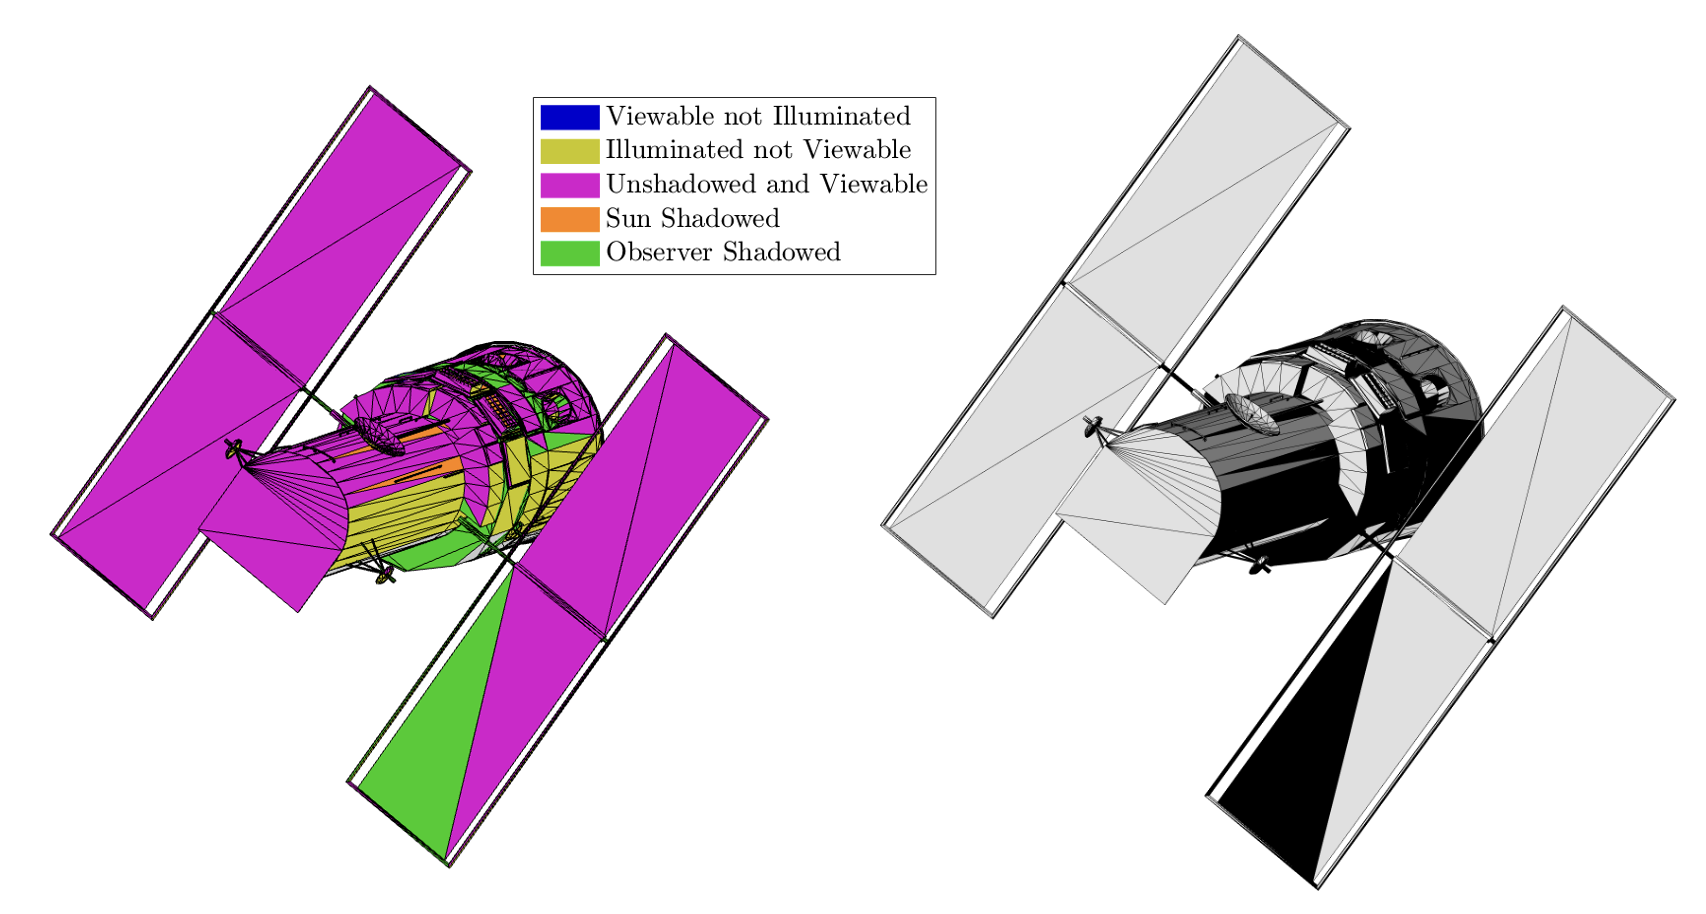
\includegraphics[width=350px]{hst_shadow_mapping/composite_hst_raytraced.png}
  \caption{Hubble Space Telescope ray traced shadow categorization and shading. Models from \cite{nasa_models}}
  \label{fig:hst_shadows_ray}
\end{figure}

The facet-wise shadow categorization shown in Figure \ref{fig:hst_shadows_ray} informs the $\mu_{ij}$ self-shadowing term in Eq \ref{eq:lc_func_normalized}. The major downside of facet-wise shadow categorization is that it is difficult to determine the fraction of each face is illuminated --- it categorizes the entire face together, leading to unphysical discontinuities in simulated light curves.

\subsubsection{The Importance of Self-Shadowing}

To motivate the need for accurate shadows when dealing with human-made space objects, consider the error introduced by neglecting shadows for different types of space objects. Kaasalainen and Torppa's work on asteroids reasonably assumed that shadowing was a negligible contribution to the measured light curve. Human-made objects do not afford the same luxury. Figure \ref{fig:hst_bennu_shadows} displays light curves for the asteroid Bennu and the Hubble Space Telescope with and without accurate shadows under a single-axis spin profile with inertially fixed Sun and observer vectors. Without accurate shadowing, the light curve's intensity and its time derivative can be significantly error-prone.

\begin{figure}[!htb]
  \centering
  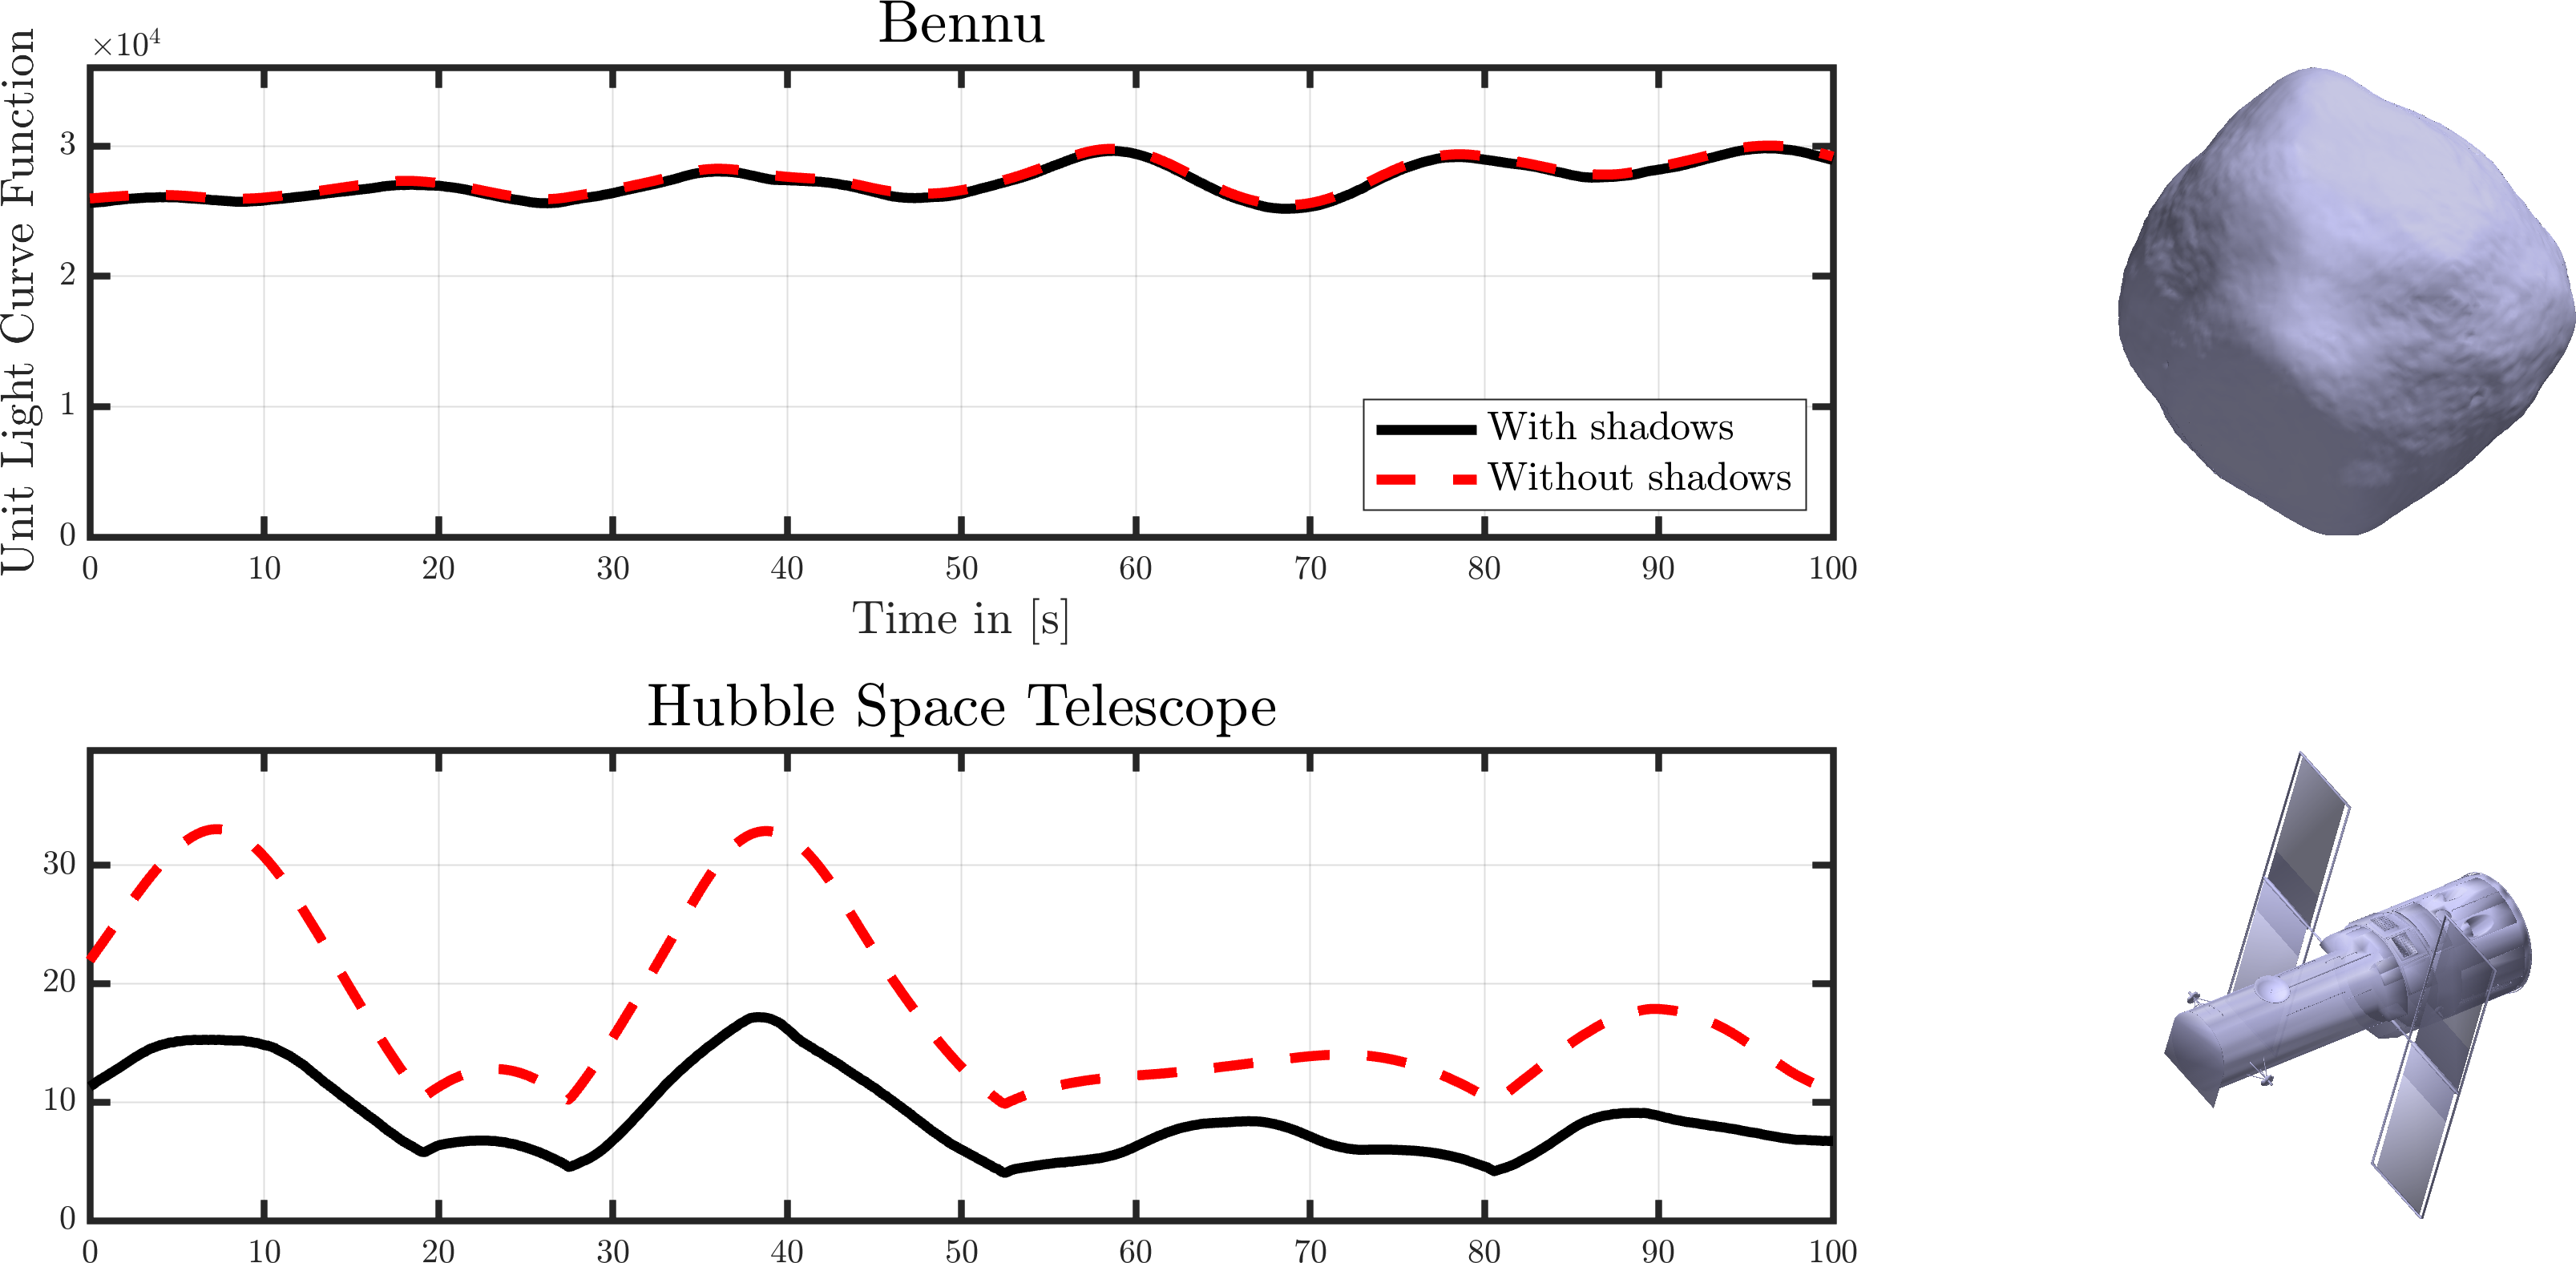
\includegraphics[width=350px]{convex_vs_nconv_lcs.png}
  \caption{Normalized irradiance errors introduced by neglecting shadows for Bennu and HST. Models from \cite{nasa_models}}
  \label{fig:hst_bennu_shadows}
\end{figure}

\subsubsection{Shadow Mapping} \label{sec:shadow_mapping}

Shadow mapping is used in the simulations presented in this work for faster and more accurate self-shadowing. Shadow mapping is a well understood technique in computer graphics \cite{kolivand2013}. Although modern ray traced shadowing may be more computationally efficient, shadow mapping was selected for its ease of implementation \cite{kolivand2013}. Shadow mapping shades individual pixel fragments instead of entire faces, offering increasing shadow quality over facewise ray tracing as the number of mesh faces falls.

Given an observer and Sun vector in the body frame of the object, shadow mapping proceeds in a four step process. In step one, a camera is positioned along the Sun vector and a perpendicular depth texture is computed. In the second step, depth values in Sun camera space are transformed to observer camera space, where a second depth texture is computed. This second texture is used to find the closest fragment along each ray to the Sun \cite{brabec2002}. Self-shadowed fragments are classified as those further from the Sun than the closest fragment along the same ray, indicated in red in Figure \ref{fig:hst_shadows_map}. Fragments that do not pass the convex shadowing condition are horizon shadowed, indicated in blue in Figure \ref{fig:hst_shadows_map}, determining the Sun and observer shadowing conditions at once. All remaining fragments are shaded with using the same Lambertian reflection model in \ref{eq:lc_func_normalized}. Computing the light curve function for the final rendered image requires summing all pixel values and dimensionalizing the result by the area of the observer camera's field of view. The light curve simulation environment used in this work was implemented in C and OpenGL \cite{raylib}.

In order to compute the final shaded and shadowed image, a depth map must be computed from the perspective of two orthographic cameras in the Sun and observer directions. These depth masks require a set of transformations from the model body frame to screen space. With this background laid out, the process for computing a perpendicular depth map $d(x,y)$ from the perspective of an arbitrary orthographic camera is detailed in Algorithm \ref{alg:depth_map}.

\begin{algorithm}
  \caption{Pixel-wise depth map computation for shadow mapping} \label{alg:depth_map}
  \begin{algorithmic}
    \State $(x, y) \in \mathbb{Z}$ \Comment{Pixel coordinates on the image plane}
    \State $R_\mathrm{pix} \in \mathbb{R}^3$ \Comment{Pixel world coordinates; provided by OpenGL}
    \State $d(x, y) \gets \left( R_{cam} - R_\mathrm{pix} \right) \cdot R_{cam}$ \Comment{Pixel depth in the camera view direction}
  \end{algorithmic}
\end{algorithm}

The pixel-wise shading process is summarized in Algorithm \ref{alg:pix_shading} in Appendix \ref{data:shading}. This shading and shadow mapping procedure is detailed graphically in Figure \ref{fig:hst_shadows_map}.

\begin{figure}[!htb]
  \centering
  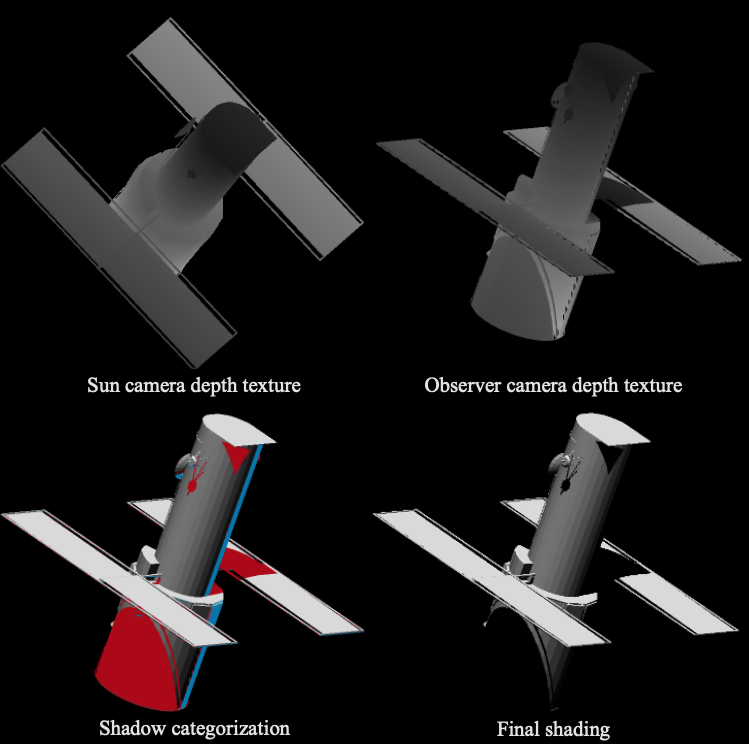
\includegraphics[width=\figmed]{hst_shadow_mapping/hst_shadow_mapping.png}
  \caption{Hubble Space Telescope shadow mapping with self (red) and horizon (blue) shadows rendered. Models from \cite{nasa_models}}
  \label{fig:hst_shadows_map}
\end{figure}
\graphicspath{{/Users/liamrobinson/Documents/PyLightCurves/docs/build/html/_images}}

An image shaded by Algorithm \ref{alg:pix_shading} is dimensionalized to a normalized irradiance value by computing the area of the square orthographic field of view given the image pixel count $n_\mathrm{pix}$:

\begin{equation} \label{eq:ortho_area}
  A_{image} = 2 n_\mathrm{pix} \left(FOV \right)^2.
\end{equation}

This field of view must be set dynamically at runtime to account for the size of the 3D model. The pixel values $v$ in the image are stored as unsigned 8 bit integers which take on values from 0 to 255, corresponding to the power range 0 to 1 within the pixel shading procedure described by Algorithm \ref{alg:pix_shading}. The total normalized irradiance in image $j$ is computed by summing over all $n_\mathrm{pix}$ pixels and dimensionalizing by the area of the image plane:

\begin{equation} \label{eq:lc_normalized_engine}
  \hat{I}_j = \frac{A_{image}}{n_\mathrm{pix}} \sum_{i=1}^{n_\mathrm{pix}}{\frac{v_{i}}{255}}
\end{equation}

\section{Simulating The Observations}

\section{Time Systems}

In order to accurately predict the position of a space object and an observer, it is necessary to understand how a given time translates to the orientation of the relevant reference frames. These calculations require conversions between various time scales, the Julian date, and sidereal time.

\subsection{Time Scales}

There are a variety of scales used to measure time. What follows is a minimal treatment of each. For a more comprehensive overview, see Section 3.5 of \cite{vallado4ed}. International Atomic Time (TAI) is based on measurements from atomic clocks and is independent of astronomical effects or observations. By definition, TAI proceeds at the rate of $1$ SI second per second. Universal Time (UT0) is derived directly from observations of the apparent position of the stars. UT1 is derived from UT0 by adjusting for polar motion. UT1 is offset from TAI by $\Delta UT1$, which is a dynamic quantity that must be continually observed. Universal Coordinated Time (UTC) is a truncation of UT1 that uses an integer number of leap seconds $\Delta AT$ to stay within $0.9$ seconds of TAI. Terrestrial Time (TT) is defined by a constant offset of $TT - TAI = 32.184$ seconds from TAI and preceding at the same rate as TAI. These time scale relations are summarized in Eq \ref{eq:time_scale_conversions}.

\begin{align*}  \label{eq:time_scale_conversions} \numberthis
  UTC &= UT1 - \Delta UT1 \\
  TAI &= UTC + \Delta AT \\
  TT &= TAI + 32.184^s \\
\end{align*}

These time scales are relevant for this research as the precise coordinate frame transformation from ITRF to the J2000.0 realization of ICRF relies on quantities expressed in UT1. Date timestamps are usually standardized to UTC, requiring the transformations in Eq \ref{eq:time_scale_conversions} for full accuracy. Figure \ref{fig:time_scales} shows the evolution of UTC, UT1, and TT with respect to TAI. Notice that $\Delta UT1$ continually changes while $\Delta AT$ is always truncated to a nearby integer.

\begin{figure}[ht]
  \centering
  \includegraphics[width=\figbig]{sphx_glr_time_systems_001.png}
  \caption{Time scales relative to TAI}
  \label{fig:time_scales}
\end{figure}

\subsection{Julian Date}

Most tasks in astrodynamics are easier when using a continuous time system. For this reason, the Julian date is adopted. This quantity is defined as the number of days elapsed since January 1, 4713 B.C., at 12:00 \cite{vallado4ed}. Given a date timestamp of the form D/M/Y h:m:s between the years of 1900 and 2100, the Julian date is computed via:

\begin{equation} \label{eq:date_to_jd}
  JD = 376Y - \fl{\left[ \frac{7Y + 7 \cdot \fl{\left(\frac{M + 9}{12} \right)}}{4} \right]}
      + \fl{\left(\frac{275M}{9}\right)} 
      + d
      + 1721013.5
      + \frac{\frac{\left(\frac{s}{60} + 60\right)}{60} + h}{24}.
\end{equation}

Note that Eq \ref{eq:date_to_jd} is always a function of the time scale used in the input, i.\,e.\, a UTC timestamp yields $JD_{UTC}$ whereas a UT1 timestamp yields $JD_{UT1}$. Another useful quantity for later time and coordinate system calculations is the number of Julian centuries since a particular epoch. The J2000.0 epoch is used unless otherwise stated, resulting in \cite{vallado4ed}:

\begin{equation} \label{eq:jd_to_t}
  T = \frac{JD - 2451545.0}{36535}.
\end{equation}

Often, more specificity is needed with respect to the time scale used in Eq \ref{eq:jd_to_t}. For example, computing $T$ with an input date in UT1 yields $T_{UT1}$ using $JD_{UT1}$, which is in turn a function of a date expressed in UT1. 

\subsection{Solar and Sidereal Time}

A solar day is defined as the time required for the Sun to pass and return to an observer's meridian --- a line of constant longitude extending from the geographic south pole to the geographic north pole \cite{vallado4ed}. By contrast, a sidereal day is the time required for the stars to complete a revolution around an observer's meridian. Due to the Earth's orbit around the Sun, the sidereal day is about 4 minutes shorter than the solar day \cite{vallado4ed}. The Greenwich mean sidereal time (GMST) is computed in seconds via \cite{frueh2019notes}:

\begin{equation} \label{eq:date_to_gmst}
  \theta_{GMST} = 67310.54841
        + \left(3.15576 \cdot 10^9 + 8640184.812866 \right) T_{UT1}
        + 0.093104 T_{UT1}^2
        - 6.2 \cdot 10^{-6} T_{UT1}^3.
\end{equation}

Accounting for the variations in the inclination of the ecliptic $\epsilon$ and the change in the equinox compared to the reference epoch $\Delta \Psi$ produces Greenwich apparent sidereal time (GAST) via \cite{frueh2019notes}:

\begin{equation} \label{eq:date_to_gast}
  \theta_{GAST} = \theta_{GMST} + \Delta \Psi \cos\epsilon.
\end{equation}

Both the inclination of the ecliptic and the difference in the equinox are computed with series expansions following the IAU 1980 theory of nutation \cite{vallado4ed}.

\section{Coordinate Systems}

A precise definition of coordinate systems is necessary for determining the position of the observer and the observed space object at a given time. The relevant conversions are summarized by a single question: how is a fixed position on the surface of the Earth transformed into a standardized inertial reference frame?

\subsection{Latitude, Longitude and Altitude}

Latitude, longitude, and altitude (LLA) is a spherical representation of position on or above the surface of the Earth. For the purposes of precise station positioning, the difference between the two types of longitude --- geocentric and geodetic --- is important. Geocentric latitude is the angle between the line from the center of mass of the Earth to the position of interest and the equatorial plane. Geodetic latitude instead measures the angle between the local ellipsoid surface normal and the equatorial plane. Geodetic latitude $\phi_\mathrm{geod}$ is converted to geocentric $\phi_\mathrm{geoc}$ latitude with \cite{frueh2019notes}:

\begin{equation} \label{eq:geod_to_geoc}
  \phi_\mathrm{geoc} = \tan^{-1} \left((1 - f)^2 \tan\phi_\mathrm{geod} \right).
\end{equation}

Additionally, the radius of the ellipsoid $r_E$ at a given geocentric latitude is necessary for later conversion, expressed by \cite{frueh2019notes}:

\begin{equation} \label{eq:rad_at_geoc}
  r_E = R_E - f \sin^2 \left( \phi_\mathrm{geoc} \right).
\end{equation}

The altitude in a set of LLA coordinates needs a reference point. Different observers may be defined differently --- either relative to the approximate ellipsoidal shape of the Earth, the hypothetical mean sea level, or the surrounding terrain.

\subsubsection{Ellipsoid}

Due to Earth's equatorial bulge, it is common to model the rough shape of the Earth as an ellipsoid. In particular, the 1984 World Geodetic Survey (WGS-84) model is used throughout this work to define the shape of the Earth ellipsoid, with parameters listed in Table \ref{tb:wgs84} for use in Eqs \ref{eq:geod_to_geoc} and \ref{eq:rad_at_geoc}.

\begin{table}[ht]
  \centering
  \begin{tabular}{|l|l|}
  \hline
  \textbf{Parameter} & \textbf{Value}              \\ \hline
  Equatorial radius $R_E$             & $6378.137 \: [km]$ \\ \hline
  Flattening ratio $f$                & $1 / 298.257$      \\ \hline
  \end{tabular}
  \caption{WGS-84 ellipsoid model of the Earth \cite{vallado4ed}.}
  \label{tb:wgs84}
\end{table}

These parameters are needed for the conversion from LLA to the International Terrestrial Reference Frame.

\subsubsection{Geoid}

The geoid accounts for the gravitational potential differences across the Earth's surface \cite{vallado4ed}. It is a surface of equal gravitational potential; the surface the ocean relaxes to without the influence of the wind and tides \cite{vallado4ed}. For this reason, the geoid is alternatively known as the mean sea level (MSL). The ellipsoid is a good approximation of the geoid, which deviates from the ellipsoid by less than $\approx 100$ meters at all latitudes and longitudes. The height of the geoid above the ellipsoid can be computed from a high-fidelity gravity model, but it is often more convenient to interpolate a pre-computed grid of geoid heights. Figure \ref{fig:geoid_shape} displays global geoid heights derived from the 1996 Earth Gravitational Model (EGM-96) relative to the ellipsoid.

\begin{figure}[ht]
  \centering
  \includegraphics[width=\figbig]{sphx_glr_geoid_heights_001_2_00x.png}
  \caption{EGM-96 geoid heights above the WGS-84 ellipsoid}
  \label{fig:geoid_shape}
\end{figure}

\subsubsection{Terrain}

Terrain elevation is usually the final component needed to fully define the altitude of a ground station, which is often defined relative to MSL. This work uses $30$-meter terrain tiles from the Shuttle Radar Topography Mission (SRTM). Figure \ref{fig:pogs_terrain} shows the local elevation around the Purdue Optical Ground Station using SRTM data.

\begin{figure}[ht]
  \centering
  \includegraphics[width=\figmed]{sphx_glr_pogs_local_terrain_001.png}
  \caption{MSL elevations surrounding the Purdue Optical Ground Station}
  \label{fig:pogs_terrain}
\end{figure}

\subsubsection{Altitude Conversions}

Given an altitude relative to the terrain $a_{terrain}$, the elevation above the ellipsoid $a_{ellip}$ is given as a function of the terrain elevation above the geoid $h_{terrain}(\lambda, \phi)$ and the geoid elevation above the ellipsoid $h_{terrain}(\lambda, \phi)$ by \cite{vallado4ed}:

\begin{equation} \label{eq:altitude_above_ellipsoid}
  a_{ellip} = a_{terrain} + h_{terrain}(\lambda, \phi_\mathrm{geod}) + h_{geoid}(\lambda, \phi_\mathrm{geod}).
\end{equation}

\subsection{International Terrestrial Reference Frame (ITRF)}

The Cartesian form of LLA is known as the Earth-centered Earth-fixed (ECEF) reference frame. Throughout this work, ECEF and ITRF will be used interchangeably. This frame has its origin at the center of mass of the Earth and its axes fixed in the crust. The
fundamental plane of the frame is defined to be the equator ---  orienting the $z$-axis through Earth's
instantaneous spin axis, and the reference direction through the intersection of the prime meridian
and the equator ---  defining the $x$-axis. Completing the right-handed system with $\hat{y} = \hat{z} \times \hat{x}$ yields a
reference frame that remains fixed, neglecting effects like continental drift. The transformation from LLA $\left( \lambda, \phi_\mathrm{geod}, a_{ellip} \right)$ to ITRF is given by \cite{vallado4ed}:

\begin{align*} \numberthis \label{eq:lla_to_itrf}
  e^2 &= 2f - f^2 \\
  N &= \frac{R_E}{\sqrt(1 - e^2 \sin(\phi_\mathrm{geod})^2)} \\
  \rho &= (N + a_{\mathrm{ellip}}) \cos(\phi_\mathrm{geod}) \\
  x_\mathrm{itrf} &= \rho \cos(\lambda) \\
  y_\mathrm{itrf} &= \rho \sin(\lambda) \\
  z_\mathrm{itrf} &= \left(N (1 - e^2) + a_{\mathrm{ellip}} \right) \sin(\phi_\mathrm{geod}). \\
\end{align*}

In Eq \ref{eq:lla_to_itrf}, $e^2$ is the squared eccentricity of the ellipsoid, $N$ is the radius of curvature in the meridian, and $\rho$ is the $x-y$ plane magnitude of the station's position \cite{vallado4ed}.

Many later transformations require the body axis rotation matrices $R_1$, $R_2$, and $R_3$ which are expressed:

\begin{align*} \numberthis \label{eq:body_rotms}
  R_1(\theta) &= \begin{bmatrix}  1 & 0 & 0 \\ 0 & \cos\theta & \sin\theta \\ 0 & -\sin\theta & \cos\theta \end{bmatrix} \\
  R_2(\theta) &= \begin{bmatrix}  \cos\theta & 0 & -\sin\theta \\ 0 & 1 & 0 \\ \sin\theta & 0 & \cos\theta \end{bmatrix} \\
  R_3(\theta) &= \begin{bmatrix}  \cos\theta & \sin\theta & 0 \\ -\sin\theta & \cos\theta & 0 \\ 0 & 0 & 1 \end{bmatrix}. \\
\end{align*}

\subsection{Topocentric East North Up (ENU) Reference Frame}

The remaining transformations in this chapter will only be defined in terms of their rotation matrices. It is often useful to express observations in a local reference frame. The East North Up (ENU) coordinate system is used throughout this work. This system has an origin at the observing station, with the first two basis vectors pointing towards the local East and North and the third pointing towards zenith. The transformation from a vector $\vctr{r}_\mathrm{itrf}$ in ITRF to $\vctr{r}_{enu}$ in ENU is a function of the longitude of the station $\lambda$ and the geocentric latitude $\phi_\mathrm{geoc}$ by \cite{frueh2019notes}:

\begin{equation} \label{eq:itrf_to_enu}
  \vctr{r}_{enu} = F_2 F_1 R_2(\phi_\mathrm{geoc}) R_3(\lambda) \vctr{r}_\mathrm{itrf}.
\end{equation}

In Eq \ref{eq:itrf_to_enu}, $R_3$ is a rotation about the third body axis, $F_1$ swaps the second and third unit vectors, and $F_2$ swaps the first and third unit vectors. The orientation of the ENU reference frame at the Purdue Optical Ground Station is depicted in Figure \ref{fig:pogs_enu}.

\begin{figure}[ht]
  \centering
  \includegraphics[width=\figmed]{sphx_glr_az_el_parallel_001.png}
  \caption{ENU reference frame orientation at Purdue Optical Ground Station}
  \label{fig:pogs_enu}
\end{figure}

\subsection{International Celestial Reference Frame (ICRF/J2000)} \label{sec:teme}

Transforming from ITRF to a standardized inertial reference frame is an involved process due to the variety of nonlinear effects impacting the Earth's rotational motion. In total, this transformation must account for polar motion, the nutation and precession of the Earth's pole, and the mean sidereal time. These transformations are treated much more thoroughly in Montenbruck and Gill \cite{montenbruck2012}. 

Accounting for polar motion --- the motion of the Earth's pole that cannot be explained through nutation theory --- transforms from $\vctr{r}_\mathrm{itrf}$ in ITRF to $\vctr{r}_{gtod}$ in Greenwich True of Date (GTOD) via \cite{vallado4ed}:

\begin{equation} \label{eq:itrf_to_gtod}
  \vctr{r}_{gtod} = R_1(y_p) R_2(x_p) \vctr{r}_\mathrm{itrf},
\end{equation}

where $x_p$ and $y_p$ are the angular components of the polar motion at the time of interest \cite{frueh2019notes}. Accounting for the sidereal rotation of the Earth about its pole transforms from $\vctr{r}_{gtod}$ in GTOD to $\vctr{r}_{teme}$ in the True Equator, Mean Equinox (TEME) reference frame via \cite{frueh2019notes}:

\begin{equation} \label{eq:gtod_to_teme}
  \vctr{r}_{teme} = R_3(-\theta_{GMST}) \vctr{r}_{gtod},
\end{equation}

where $\theta_{GMST}$ is the Greenwich mean sidereal time. Accounting for the difference between GMST and GAST at the date of interest transforms $\vctr{r}_{teme}$ TEME to $\vctr{r}_{tod}$ in the True of Date (TOD) reference frame via \cite{vallado4ed}:

\begin{equation} \label{eq:teme_to_tod}
  \vctr{r}_{tod} = R_3(-\Delta \Psi \cos \epsilon) \vctr{r}_{teme},
\end{equation}

where $\Delta \Psi$ is the angular difference in the longitude of the vernal equinox between GMST and GAST, and $\epsilon$ is the true inclination of the ecliptic \cite{vallado4ed}. Accounting for the nutation of Earth's pole transforms $\vctr{r}_{tod}$ from TOD to $\vctr{r}_{mod}$ in the Mean of Date (MOD) reference frame via \cite{vallado4ed}:

\begin{equation} \label{eq:tod_to_mod}
  \vctr{r}_{mod} = R_1(-\bar{\epsilon}) R_3(\Delta\Psi) R_1(\bar{\epsilon} + \Delta\epsilon) \vctr{r}_{tod},
\end{equation}

where $\bar{\epsilon}$ is the mean inclination of the ecliptic at the time of interest, and $\epsilon$ is the true inclination of the ecliptic \cite{vallado4ed}.

Accounting for the secular precession of Earth's pole transforms $\vctr{r}_{mod}$ from MOD to $\vctr{r}_\mathrm{icrf}$ in ICRF via \cite{vallado4ed}:

\begin{equation} \label{eq:mod_to_icrf}
  \vctr{r}_\mathrm{icrf} = R_3(\zeta) R_2(\theta) R_3(z) \vctr{r}_{mod},
\end{equation}

through the 3-2-3 Euler angle sequence $\left( z, \theta, \zeta \right)$. Each of these angles modeling the precession are a function of the date of the transformation, and are approximated by polynomial expansions in the Julian century $T$ \cite{frueh2019notes}.

The specific realization of ICRF used in this work is referenced to the position of the equator and equinox at the J2000.0 epoch (January 1, 2000 12:00:00.000 TT), leading to the common name for this reference frame, "J2000" \cite{vallado4ed}.

\subsection{Right Ascension and Declination}

Right ascension and declination, often shortened to RA/Dec, are useful angles for describing the angular position of an object on the celestial sphere from the perspective of an observer. As such, RA/Dec values are inertial, but can be defined relative to a topocentric observer or the center of the Earth \cite{frueh2019notes}. The topocentric RA/Dec is exclusively used in this work for later simulations. Right ascension is defined as the angle
of the observation projected onto the inertial $x-y$ plane, measured counterclockwise from inertial
$\hat{x}$, represented by $\alpha$. Declination is the angle from the $x-y$ plane to the observation
with positive values above the $x-y$ plane (closer to inertial $z$) and negative values below.
Declination is represented by $\delta$. Given a unit vector direction $\hat{v} = \left[ x_\mathrm{itrf}, y_\mathrm{itrf}, z_\mathrm{itrf} \right]^T$ in J2000, RA/Dec is computed via \cite{frueh2019notes}:

\begin{equation} \label{eq:eci_to_ra_dec}
  \begin{bmatrix}
	\alpha \\
	\delta
  \end{bmatrix} = 
  \begin{bmatrix}
	\atantwo(y_\mathrm{itrf}, x_\mathrm{itrf}) \\
	\atantwo(z_\mathrm{itrf}, \sqrt{x_\mathrm{itrf}^2 + y_\mathrm{itrf}^2})
  \end{bmatrix}.
\end{equation}

\subsection{Azimuth and Elevation}

Azimuth and elevation, often shortened to Az/El, are similar angular quantities to right ascension and declination \cite{frueh2019notes}. Instead of being based on
the inertial sphere, they are referenced to an arbitrary reference frame. For a telescope making
observations of an object, the local topocentric ENU frame may be used. For a satellite star
tracker, star azimuth and elevation might be reported in the satellite body frame. In either case,
Eq \ref{eq:eci_to_ra_dec} can be repurposed in terms of Az/El, where $\hat{v} = \left[ x_{ENU}, y_{ENU}, z_{ENU}
\right]^T$ is expressed in the frame of interest \cite{frueh2019notes}.

\begin{equation} \label{eq:enu_to_az_el}
  \begin{bmatrix}
	Az \\
	El
  \end{bmatrix} = 
  \begin{bmatrix}
	\atantwo(y_{ENU}, x_{ENU}) \\
	\atantwo(z_{ENU}, \sqrt{x_{ENU}^2 + y_{ENU}^2})
  \end{bmatrix}
\end{equation}

Note that Eq \ref{eq:enu_to_az_el} references azimuth to the $x$-axis, proceeding in the
counterclockwise direction. Often, this reference axis and direction may be changed depending on the
reference frame being used. For example, ground station observations may be referenced to local
North ---  the second axis of the ENU system ---  proceeding clockwise. This would require the
substitution $Az' = \frac{\pi}{2} - Az$. Notice that this substitution leads to $Az'$ leaking
outside the domain of $[0, 2\pi)$. This is not an issue for later coordinate transformations but
may be undesirable for plots. Wrapping the result back to the standard azimuth range via
$Az_{wrapped} = \textrm{mod}(Az, 2\pi)$ is a sufficient fix.

\subsection{Coordinate Transformations Summary}

With these transformations, any topocentric observation directions in RA/Dec or Az/El can be converted into a Cartesian representation and transformed into J2000. Simultaneously, any propagated space object orbits can be transformed similarly from an arbitrary propagation frame such that all future computations requiring the observation geometry take place in the same reference frame. 

\subsection{Planetary Ephemerides} \label{sec:planet_ephem}

The Spacecraft, Planet, Instrument, C-matrix, and Events (SPICE) toolkit is used for the propagation of the Sun and Moon throughout the results presented in this work \cite{spice}. SPICE is maintained by the NASA Jet Propulsion Laboratory's Navigation and Ancillary Information Facility (NAIF) and provides the state of the art solutions for the positions and orientations of solar system bodies \cite{spice}. All calculations of $\vctr{r}_{Sun}$ and $\vctr{r}_\mathrm{Moon}$ rely on queries to SPICE using the DE440s planetary ephemeris files.

\section{The Charge Coupled Device (CCD)} \label{sec:ccd_performance}

Many optical telescopes, including the Purdue Optical Ground Station, use a CCD to convert incident photons into a digital signal on a pixel grid \cite{krag2003}. CCDs accomplish this with a matrix of semiconductor pixel wells which collect electrons released by the photoelectric effect when photons are incident on that pixel \cite{krag2003}. The release of these photoelectrons is wavelength dependent and is captured by the quantum efficiency spectrum of a given CCD. Developing this background in photometry is useful for both light curve simulation as well as simulating the CCD camera measuring that light curve. 

Due to the sheer distance from the observer to any space object, taking an image that resolves the object's geometry is generally impossible. For an observer with the pixel scale of the Purdue Optical Ground Station ($s_\mathrm{pix} = 0.72 \: [arcsec/pixel]$), a 6U CubeSat in LEO occupies about 1/44 of a pixel area, while a large communications satellite in GEO occupies approximately 1/13 of a pixel area. In either case, no geometric information is left on the image plane even before diffraction is taken into account. 

Whenever an optical telescope is observing an unresolved space object, the object's signal is necessarily superimposed on whatever signals exist in the background as the unresolved signal spreads much farther than the object's actual geometric bounds. In this context, background does not only refer to sources physically further than the object --- as light can easily enter optical path through atmospheric scattering --- but all sources that impact the image apart from the object signal. Some of these sources even originate within the telescope optics and its sensor. To faithfully simulate a telescope observing an object, many position-based SDA tasks are able to ignore background effects while acquiring or tracking objects. For photometry-based SDA, the background is critical. The overall noise floor can be broken up into background signal sources and sensor effects.

\subsection{Diffraction}

Many objects of interest are far past LEO, making optical observations diffraction limited. Diffraction is always occurring when observing an object at any distance through any optics, but it begins to dominate when the object's scale is equal or smaller than the Rayleigh criterion \cite{frueh2019notes}.

\subsubsection{Rayleigh Criterion}

The Rayleigh criterion states that light of wavelength $\lambda$ will spread into a diffraction pattern with the first minimum of the distribution at an angular radius $\theta_R$ when passing through a circular aperture of diameter $d$ \cite{frueh2019notes} such that:

\begin{align*} \numberthis \label{eq:rayleigh_criterion}
  \sin\theta_R &= \frac{1.22 \lambda}{d}, \\
  \theta_R &\approx \frac{1.22 \lambda}{d}.
\end{align*}

For a $0.5$-meter aperture optical telescope with a pixel scale of $1$ arcsecond per pixel, observing a $40$-meter wide object in GEO --- occupying approximately $0.2$ pixel widths on the image --- Eq \ref{eq:rayleigh_criterion} predicts that the diffraction pattern will be $2.4$ times wider than the object at a wavelength of $550$ nanometers. Similarly, a $60$-centimeter wide object in LEO observed with the same telescope occupies $0.1$ pixel widths in the image while producing an Airy disk $4.5$ times wider than the object itself. As a result, GEO objects cannot be resolved from the ground, independent of atmospheric effects. 

\subsubsection{The Airy Disk}

The far-field diffraction pattern produced by a point source is known as an Airy pattern or disk \cite{frueh2019notes}. The Airy disk is expressed in terms of an amplitude $C$ at an angular distance $\theta$ from the center $C(\theta)$ \cite{frueh2019notes} as:

\begin{equation} \label{eq:airy_disk}
  C_{Airy}(\theta) = C_0 \left( \frac{2 J_1(k \cdot r_d \sin\theta)}{k \cdot r_d \sin\theta} \right).
\end{equation}

In Eq \ref{eq:airy_disk}, $C_0$ is the amplitude of the center of the Airy disk, $r_d$ is the radius of the aperture, $k = \frac{2\pi}{\lambda}$ is the wavenumber, and $J_1$ is the first order Bessel function of the first kind. The central magnitude $C_0$ is expressed:

\begin{equation} \label{eq:airy_center}
  C_0 = \frac{S_\mathrm{obj}^2 A_\mathrm{aperture}^2}{2 f^4}.
\end{equation}

In Eq \ref{eq:airy_center}, $S_\mathrm{obj}$ is the total mean irradiance incident on the CCD due to the source, $A_\mathrm{aperture}$ is the aperture area, and $f$ is the focal length of the optics \cite{frueh2019notes}. The pattern produced by Eq \ref{eq:airy_disk} is depicted in Figure \ref{fig:airy_disk_magnitude}.

\begin{figure}[ht]
  \centering
  \includegraphics[width=\figmed]{sphx_glr_airy_disk_diffraction_001_2_00x.png}
  \caption{Airy disk diffraction pattern}
  \label{fig:airy_disk_magnitude}
\end{figure}

The Rayleigh criterion expresses the angular size of the first zero of the Airy disk, after which the amplitude of the Airy disk drops off exponentially. It is often useful to approximate the Airy disk with a 2D Gaussian. Given the total signal to be approximated, this Gaussian is fit with a single parameter --- the full width at half maximum (FWHM). The FWHM expresses the diameter at which the signal drops to half the magnitude of its central maximum \cite{frueh2019notes}. The FWHM of the Airy disk is expressed \cite{frueh2019notes}:

\begin{equation} \label{eq:fwhm_airy}
  FWHM_\mathrm{Airy} = \frac{1.028 \lambda}{2 r_d}.
\end{equation}

The diffraction pattern is not the only effect that spreads the unresolved signal over the pixel grid. Atmospheric turbulence contributes to further spreading and speckling of the signal \cite{frueh2019notes}. This effect --- known as the \textit{seeing} --- is encapsulated in $FWHM_{seeing}$ and is generally between $1$ and $3$ arcseconds \cite{frueh2019notes}. While the seeing and diffraction pattern FWHMs are additive, it is sufficient to take the larger value for simulation purposes \cite{frueh2019notes}. The standard deviation of the Gaussian approximation of the Airy disk is given by:

\begin{equation} \label{eq:airy_variance}
  \sigma = \frac{FWHM}{2 \sqrt{2 \ln{2}}}.
\end{equation}

The full Gaussian approximation at an angular distance $\theta$ from the source is given by:

\begin{equation} \label{eq:airy_gaussian}
  C_{Gauss}(\theta) = \frac{0.838 \bar{C}_\mathrm{all}}{2 \pi \sigma^2} \exp\left( - \frac{\theta^2}{2 \sigma^2} \right)
\end{equation}

In practice, computing the Airy disk or its Gaussian approximation on rectangular pixel grid amounts to integrating the amplitude function $C(\theta)$ over the pixel area:

\begin{equation} \label{eq:pix_values_gauss}
  C_\mathrm{pix}(x, y) = \int_{x}^{x + \Delta x} \int_{y}^{y + \Delta y}{C_{Gauss}(\theta(x, y))} \: dy \: dy.
\end{equation}

The area within the first maximum of the Airy disk is given by \cite{frueh2019notes}:

\begin{equation} \label{eq:airy_area}
  A_\mathrm{Airy} = \pi \left(\frac{648000 / \pi}{s_\mathrm{pix}} \sin^{-1}\left(\frac{1.22 \lambda}{D}\right) \right)^2.
\end{equation}

\subsection{Signal-to-Noise Ratio (SNR)}

Because the unresolved object signals are always superimposed on the background of the image, the SNR of a CCD is expressed with the signal included in the denominator noise term \cite{frueh2019notes}:

\begin{equation} \label{eq:ccd_snr}
  SNR = \frac{S_\mathrm{obj}}{\sqrt{S_\mathrm{obj}+N}}.
\end{equation}

Explicitly, the SNR can be expanded in terms of the signal means and variances, assuming that their respective probability density functions are independent \cite{frueh2019notes}:

\begin{equation} \label{eq:ccd_snr_expanded}
  SNR = \frac{S_\mathrm{obj}}{\sqrt{S_\mathrm{obj} + n_\mathrm{pix} \left( \lambda_\mathrm{background} + \lambda_{dark} + \sigma^2_\mathrm{read} + \frac{g^2}{24} \right)}}.
\end{equation}

It should be noted that the SNR computed in Eq \ref{eq:ccd_snr_expanded} is idealized. In reality, the discrete sampling of each random variable in each object pixel --- as well as the Poisson sampling of the object signal --- results in a slightly different value. As the number of object pixels approaches infinity, the SNR computed from the image would approach the theoretical value. Figure \ref{fig:snr_grid} illustrates the effect of raising the background noise level while holding the object signal constant on the SNR.

\begin{figure}[ht]
  \centering
  \includegraphics[width=\figmed]{sphx_glr_snr_001_2_00x.png}
  \caption{Signal-to-noise ratio reduction on a synthetic CCD pixel grid}
  \label{fig:snr_grid}
\end{figure}

The SNR is an important constraint when determining whether an object signal is visible above the background. If the SNR is too low, it becomes difficult or impossible to notice and quantify the object signal. Simulations in this work are all performed with a reasonable SNR limit of $3$.

\subsection{Telescope Properties} \label{sec:telescope_properties}

While much of the focus in this work is directed towards the CCD, the telescope it is mounted within has a few important properties which must be known for accurate CCD simulation. 

The aperture of the telescope is the beginning of the optical path within the telescope --- the area that collects incoming light. The area of the aperture $A_\mathrm{aperture} = \pi r_{d}^2$, where $r_d$ is the radius of the aperture must be distinguished from the \textit{effective} aperture area, which is the total area of the aperture which actually collects light. Some telescopes have central obstructions which remove an amount of aperture area from the optical path, such that the effective aperture area is:

\begin{equation}
  A_\mathrm{eff} = A_\mathrm{aperture} - \pi r_{o}^2,
\end{equation}

where $r_o$ is the radius of the obstruction. The telescope focal length $f$ is the length of the optical path within the optics required to resolve a focused image. The pixel scale $s_\mathrm{pix}$ is a measure of the angle spanned by the side length of each square pixel, often expressed in arcseconds per pixel. 

\subsection{Brightness Units}

In the context of photometry, "brightness" is a catch-all term for a variety of units. Defining the relationships between these units will make later light curve conversions more clear. Brightness conversions are needed for both light curves and the environmental data sources that drive the CCD performance model described in Section \ref{sec:ccd_performance}.

\subsubsection{$\mathbf{S_{10}}$ Surface Brightness}

While apparent magnitude and irradiance are effective for quantifying the flux of point sources, other units exist
to describe diffuse or extended sources where brightness is spread over an
area. $S_{10}$ is a unit of surface brightness representing the number of 10th magnitude stars per square degree that would produce the same flux as a given diffuse source.
Surface brightness in $S_{10}$ over a given solid angle $\Omega \: \left[ sr \right]$ can be converted to total irradiance $I \: \left[ \frac{W}{m^2} \right]$ via \cite{krag2003}:

\begin{equation} \label{eq:s10toirrad}
 \frac{I \left[ \frac{W}{m^2} \right]}{S_{10}} = 10^{-10/2.5} \left( \Omega \frac{180^2}{\pi^2} \right)
  \int_{10^{-8}}^{10^{-6}}{ \textrm{STRINT}(\lambda) \: d\lambda} = 8.26617 \Omega \cdot 10^{-9}.
\end{equation}

In \ref{eq:s10toirrad}, $\textrm{STRINT}(\lambda) \: \left[ \frac{W}{m^2 \cdot m} \right]$ is the
representative spectrum of a 0th magnitude star, $\textrm{QE}(\lambda)$ is the quantum efficiency
spectrum of the observing sensor, $\textrm{ATM}(\lambda)$ is the atmospheric transmission spectrum, $\lambda \: [m]$ is wavelength, $h \: \left[
\frac{m^2 \cdot kg}{s} \right]$ is Plank's constant, and $c \: \left[ \frac{m}{s^2} \right]$ is the
speed of light in vacuum. Quantum efficiency has units of photoelectrons, conveying the fraction of incident photons converted to photoelectrons in the CCD sensor. Atmospheric transmission is a unitless quantity conveying the fraction of light that is not absorbed by the atmosphere. Example spectra for $\textrm{ATM}(\lambda)$ and $\textrm{QE}(\lambda)$ are displayed in Figure \ref{fig:spectra}, with underlying data provided in Appendix \ref{data:atm}.

\subsubsection{Magnitude per Square Arcsecond}

A second surface brightness unit is $\left[ \frac{mag}{arcsec^2} \right]$, also known as MPSAS (magnitude per square arcsecond) \cite{krag2003}. This quantity can be thought of as a generalized $S_{10}$, where instead of quantifying the number of stars of a certain
magnitude in a solid angle, the equivalent magnitude of a single point source is measured. A surface
brightness $B_{10}$ in $S_{10}$ can be converted into surface brightness $B_{mag}$ in 
$\left[ \frac{mag}{arcsec^2} \right]$ by applying Eq \ref{eq:mag_to_irradiance}.

\begin{equation} \label{s10_to_mag_per_a2}
	B_{mag} = -2.5 \log_{10}\left( \frac{B_{10} \cdot 10^{-4}}{12960000} \right).
\end{equation}

In Eq \ref{s10_to_mag_per_a2} $B_{10}$ is converted to the total irradiance per square degree,
converted square degrees to square arcseconds, and finally transformed into apparent magnitude. MPSAS is converted to irradiance per steradian using \ref{eq:mag_to_irradiance}:

\begin{equation} \label{eq:mpsas_to_irrad_per_ster}
  I = \left( \frac{180}{ 3600\pi} \right)^2 I_s \cdot 10^{-\frac{MPSAS}{2.5}}.
\end{equation}

\subsubsection{Candela} \label{sec:candela}

Some light pollution datasets are given in units that include candela. Candela is the SI base unit of luminous intensity defined by the International Committee for Weights and Measures as "Fixing the numerical value of the luminous efficacy of monochromatic radiation of frequency $540\cdot10^{12}$ Hz to be equal to exactly $683$" \cite{nist_units}. This means that an isotropic green light source with frequency $540\cdot10^{12}$ Hz ($\lambda = 555$ nm) has a luminous efficacy of $K_{cd} = 683 \: \left[ lm/W \right]$ where lm stands for lumens. Luminous efficacy itself determines how well a source produces visible light. For a given wavelength, candela $B_{cd}$ is converted to watts per steradian $B_{wsr}$ via \cite{nist_units}:

\begin{equation} \label{eq:cd_to_w_per_sr}
  B_{wsr}(\lambda) = \frac{B_{cd}}{K_{cd}(\lambda)}.
\end{equation}

The luminous efficiency function $K_{cd}(\lambda)$ models the human eye's response to the visible spectrum \cite{sharpe2005}. Different fits of this function exist; the function proposed by Sharpe et al.\ is adopted, displayed in Figure \ref{fig:luminous_efficiency} \cite{sharpe2005}.

\begin{figure}[ht]
  \centering
  \includegraphics[width=\figmed]{sphx_glr_luminous_efficiency_001_2_00x.png}
  \caption{Luminous efficiency function from \cite{sharpe2005}}
  \label{fig:luminous_efficiency}
\end{figure}

Candela per unit area can be converted into MPSAS by combining Eq \ref{eq:cd_to_w_per_sr} with \ref{eq:irradiance_to_mag}, yielding a formulation which is still a function of the source's wavelength:

\begin{equation} \label{eq:cd_per_m2_to_mpsas}
  MPSAS(\lambda) = -2.5 \log_{10}\left( \frac{B_{cd}}{\left( \frac{180}{ 3600\pi} \right)^2 K_{cd}(\lambda) I_s} \right).
\end{equation}

\subsubsection{Photoelectron Counts}

Accurately simulating measured light curves requires an accurate simulation of the CCD camera taking the image. The first step towards that is understanding how irradiance at the telescope aperture is converted into pixel values in the final image. Raw images taken by a CCD-equipped telescope have pixel values measured in photoelectron counts, otherwise known as Analog-to-Digital Units (ADU) \cite{krag2003}. The count in a single pixel obtained is directly proportional (via the CCD's gain) to the number of
photons incident on that pixel during the integration time \cite{krag2003}. Higher order effects in the silicon of
the CCD renders this description incomplete, but for non-resolved imaging applications
concerned about, effects smaller than the sensor readout noise and dark current can be safely neglected
\cite{frueh2019notes}. Irradiance can be converted to ADU via the conversion factor $\mathcal{S}_\mathrm{int}$
through \cite{krag2003}:

\begin{equation} \label{eq:sint}
 \mathcal{S}_\mathrm{int} = A_\mathrm{eff}
	\int_{10^{-8}}^{10^{-6}}{ \left( \frac{\textrm{SUN}(\lambda)}{I_{sun}} \right) \cdot \textrm{QE}(\lambda) \cdot \textrm{ATM}(\lambda)
  \cdot \left( \frac{\lambda}{h c} \right) \: d\lambda}.
\end{equation}

In Eq \ref{eq:sint}, $\textrm{SUN}(\lambda)$ is the spectrum of solar irradiance in 
$\left[\frac{W}{m^2\cdot m} \right]$, $I_{sun}$ is the irradiance of the Sun, generally taken to be
the solar constant $1361 \: \left[ \frac{W}{m^2} \right]$, and $A_\mathrm{eff}$ is the effective aperture area. Read literally, the integral term has
units $\left[ \frac{1}{Ws} \right]$, giving the number of counts per incident Watt of solar
radiation and second of integration time. The aperture diameter factor outside the integral accounts
for the area of light incident on the CCD, giving $\mathcal{S}_\mathrm{int}$ units of $\left[ \frac{m^2}{Ws}
\right]$. The spectra in Eq \ref{eq:sint} are plotted in Figure \ref{fig:spectra} with data in Appendix \ref{data:spectra}. Multiplying by irradiance in $\left[ \frac{W}{m^2} \right]$ and an integration time $\Delta t$ 
in seconds will yield the mean photoelectron signal $\bar{C}_\mathrm{all}$ in ADU via:

\begin{equation} \label{eq:irrad_to_count}
  \bar{C}_\mathrm{all} = \mathcal{S}_\mathrm{int} \cdot I \cdot \Delta t.
\end{equation}

For completeness, irradiance can be recovered from a signal in ADU and the integration time:

\begin{equation} \label{eq:count_to_irrad}
  I = \frac{S}{\mathcal{S}_\mathrm{int}} \cdot \Delta t.
\end{equation}

\subsection{Background Signal Sources}

\subsubsection{Background Source Importance}

Some background signals are more impactful than others. For simulating realistic light curves, it is important to only model those background sources that have the possibility of being at or above the order of magnitude of the object signal, thereby seriously degrading the signal-to-noise ratio. As a baseline, the background terms modeled by Krag for the PROOF CCD performance model were implemented, namely scattered moonlight, airglow, zodiacal light, and integrated starlight \cite{krag2003}. In addition, twilight and light pollution models were implemented to increase the time and station location flexibility of the simulation. Each background term is modeled at medium fidelity --- often using tabulated measurements or a set of exponential distributions to govern the scattering physics. As a result, this background performance model does not capture local weather conditions or precisely simulate the scattering of each photon through the atmosphere, but still strives to faithfully model the physics of each background signal process. Table \ref{tb:signal_importance} ranks the approximate magnitudes in photoelectrons per pixel one can expect from a telescope similar to the Purdue Optical Ground Station.

\begin{table}[]
  \centering
  \begin{tabular}{|l|l|}
  \hline
  \textbf{Source} & \textbf{Magnitude} $\mathbf{\left[ e^- / \textbf{pix}\right]}$ \\ \hline
  Twilight               & $10^1 - 10^7$                              \\ \hline
  Scattered moonlight    & $0 - 10^5$                                 \\ \hline
  Airglow                & $10^3 - 10^4$                              \\ \hline
  Zodiacal light         & $10^2 - 10^4$                              \\ \hline
  Light pollution        & $10^2 - 10^3$                              \\ \hline
  Integrated starlight   & $10^1 - 10^2$                              \\ \hline
  \end{tabular}
  \caption{Background signal importance, values generated by the author using models by Krag and Daniels \cite{krag2003, daniels1977}}
  \label{tb:signal_importance}
\end{table}

\subsubsection{Astronomical Spectra}

Four of the quantities needed for the background model vary with wavelength. These are the atmospheric transmission, the sensor quantum efficiency, the irradiance of a 0th magnitude star, and the solar spectrum. Each spectrum is displayed in Figure \ref{fig:spectra}.

\begin{figure}[ht]
  \centering
  \includegraphics[width=\figmed]{sphx_glr_astro_spectra_001_2_00x.png}
  \caption{Astronomical Spectra, atmospheric transmission and zero magnitude stellar spectrum from \cite{krag2003}}
  \label{fig:spectra}
\end{figure}

In practice, the quantum efficiency curve varies by sensor and the thermal conditions of the
observation. The curve adopted in this work is that used by Krag; modern sensors will often
perform better.

\subsubsection{Airglow}

Certain chemical reactions from 80-110 km altitude in the upper atmosphere release visible light
\cite{krag2003}. This effect is known as
airglow. Since these reactions are assumed to be isotropic ---  equally intense when integrated along any
vertical line extending upwards from the surface. The airglow signal $\mathcal{A}_\mathrm{int}$ is modeled in a
similar fashion to integrated starlight. Given the airglow spectra $\mathcal{A}(\lambda) \:
\left[ \frac{W}{m^2\cdot m \cdot sr} \right]$, the sensor quantum efficiency $\textrm{QE}(\lambda)$, the atmospheric transmission $\textrm{ATM}(\lambda)$, as well as Plank's constant $h$ and the speed of light in vacuum $c$, the airglow signal is computed via \cite{krag2003}:

\begin{equation} \label{eq:aint}
 \mathcal{A}_\mathrm{int} = A_\mathrm{aperture}
  \int_{10^{-8}}^{10^{-6}}{ \mathcal{A}(\lambda) \cdot \textrm{QE}(\lambda) \cdot \textrm{ATM}(\lambda)
  \cdot \left( \frac{\lambda}{h c} \right) \: d\lambda}.
\end{equation}

The quantity $\mathcal{A}_\mathrm{int}$ has units $\left[ \frac{1}{s\cdot sr} \right]$, meaning that the
mean airglow signal in ADU per pixel is simply given by:

\begin{equation} \label{eq:airglow_adu}
  \bar{S}_{airglow} = \mathcal{A}_\mathrm{int} \cdot \textrm{AM}(\theta_z) \cdot \Delta t \cdot \left( \frac{\pi s_\mathrm{pix}}{648000} \right)^2.
\end{equation}

In Eq \ref{eq:airglow_adu}, $\textrm{AM}(\theta_z)$ is the relative airmass function which accounts for the accumulation of air along the optical path at different zenith angles \cite{frueh2019notes}. This airmass is termed \textit{relative} as it relates the ratio of absolute airmass at a zenith angle to the absolute airmass at zenith. Often, this function is approximated by the Van-Rhijn factor $\textrm{AM}(\theta_z) = \sec{\theta_z}$, which remains accurate up to $\theta_z \approx 70^\circ$ before diverging to infinity. Instead, a function proposed by Pickering is used \cite{pickering2002}.

\begin{equation} \label{eq:pickering_airmass}
  \textrm{AM}(\theta_z) = \frac{1}{\sin\left((90 - \theta_z) +  \frac{244}{165 + 47 \left(90 - \theta_z \right)^{1.1}}\right)}
\end{equation}


Using Eq \ref{eq:pickering_airmass} instead of the Van-Rhijn factor enables the computation of background signals near the horizon without the singularity of $\sec \theta$. Figure \ref{fig:airmass_fcns} displays this comparison in action.

\begin{figure}[ht]
  \centering
  \includegraphics[width=\figmed]{sphx_glr_vr_factor_001.png}
  \caption{Airmass function comparison. The Van-Rhijn factor diverges to $+\infty$ while Pickering's function reaches the correct maximum of $\textrm{AM}(\theta_z) \approx 40$.}
  \label{fig:airmass_fcns}
\end{figure}

\begin{figure}[ht]
  \centering
  \includegraphics[width=\figmed]{sphx_glr_background_signals_005.png}
  \caption{Mean airglow signal on the local observer hemisphere. The observer is in New Mexico, USA at
  \pogslla}
  \label{fig:airglowhemi}
\end{figure}

\subsubsection{Light Pollution}

Another source of background noise is light pollution. On a cloudless night with low levels of atmospheric aerosols, 
the zenith surface brightness is approximately $22 \: \left[ \frac{mag}{arcsec^2}
\right]$ (MPSAS) \cite{krag2003}. As light pollution increases, this zenith brightness may dip down to
$14-15 \: \left[ \frac{mag}{arcsec^2} \right]$. To get accurate localized zenith brightness values,
 the 2015 World Atlas of Sky Brightness dataset is used \cite{falchi2016_data}. The data is reported in $\left[
	\frac{mcd}{cm^2} \right]$ on a 30-arcsecond grid, requiring conversion to a more useful unit. A subset of the global dataset is displayed in \ref{fig:pollution_data} This conversion is listed in Eq \ref{eq:cd_per_m2_to_mpsas}, using a monochromatic $\lambda = 474$ nm to fit the conversions of Falchi et al.\ \cite{falchi2016}.  

\begin{figure}[ht]
  \centering
  \includegraphics[width=\figmed]{sphx_glr_nightlights_001_2_00x.png}
  \caption{Zenith light pollution in the eastern USA, data from \cite{falchi2016_data}}
  \label{fig:pollution_data}
\end{figure}

The mean light pollution CCD signal in ADU per pixel is formulated similarly to airglow. The station's zenith surface brightness $B_{\mathrm{poll},z}$ in MPSAS, linearly interpolated from the World Atlas dataset, is converted to irradiance per steradian via \ref{eq:mpsas_to_irrad_per_ster} and to ADU per pixel via:
 
\begin{equation} \label{eq:pollution_adu}
  \bar{S}_{pollution} = B_{\mathrm{poll},z} \cdot \mathcal{S}_\mathrm{int} \cdot \textrm{AM}(\theta_z) \cdot \Delta t \cdot \left( \frac{\pi s_\mathrm{pix}}{648000} \right)^2.
\end{equation}

Note that Krag does not implement a specific light pollution model, but instead takes the dark sky site zenith brightness of $22$ MPSAS as input to an atmospherically scattered light model \cite{krag2003}. The formulation of the light pollution model in Eq \ref{eq:pollution_adu} is simply an adaptation of Krag's model with a variable zenith brightness driven by a light pollution dataset.

\begin{figure}[ht]
  \centering
  \includegraphics[width=\figmed]{sphx_glr_background_signals_003.png}
  \caption{Mean light pollution signal on the local observer hemisphere. The observer is in New Mexico, USA at
  \pogslla}
  \label{fig:pollution_hemi}
\end{figure}

\subsubsection{Twilight}

Even after the Sun sets, scattered sunlight in the upper atmosphere creates a signal on the CCD. The twilight model implemented for this work is due to Patat et al.\ and was developed for the European Southern Observatory at Paranal in Chile \cite{patat2006}. This model implements the zenith brightness as a function of the solar zenith angle $\gamma$ --- the angle from zenith to the Sun's apparent centroid. The model of Patat et al.\ fits a second-degree polynomial in $\gamma$ to approximately 2000 observations in varying atmospheric conditions, yielding separate curves for each of the UBVRI passbands. For example, for the V band, the twilight zenith brightness in MPSAS is given by \cite{patat2006}:

\begin{equation} \label{eq:b_zenith_twilight}
  B_{twi,z} = 11.84 + 1.518(\gamma - 95^\circ) - 0.057 (\gamma -  95^\circ)^2.
\end{equation}

Eq \ref{eq:b_zenith_twilight} is valid from $95^\circ \leq \gamma \leq 105^\circ$. While $\gamma \le 95^\circ$, the zenith brightness is taken to be constant and equal to the brightness at $\gamma = 95^\circ$. This is not accurate, as it predicts daylight to be the brightness of twilight, but is sufficiently bright to correctly forbid daytime observations by lowering the SNR drastically. After $\gamma = 105^\circ$ the zenith surface brightness is set to $B_{twi,z} = 22$ MPSAS to match the optimal observation condition of the light pollution model \cite{krag2003}. Zenith twilight brightness is plotted as a function of $\gamma$ in Figure \ref{fig:twilight_model}.

\begin{figure}[ht]
  \centering
  \includegraphics[width=\figmed]{sphx_glr_twilight_model_001_2_00x.png}
  \caption{Twilight model surface brightness at zenith as a function of solar zenith angle}
  \label{fig:twilight_model}
\end{figure}

Computing the mean CCD signal in ADU per pixel due to the twilight brightness proceeds identically to the light pollution formulation. 

\begin{equation} \label{eq:twilight_adu}
  \bar{S}_{twilight} = B_{twi,z} \cdot \mathcal{S}_\mathrm{int} \cdot \textrm{AM}(\theta_z) \cdot \Delta t \cdot \left( \frac{\pi s_\mathrm{pix}}{648000} \right)^2
\end{equation}

The mean twilight signal on the local observer hemisphere is displayed in Figure \ref{fig:twilight_hemi}.

\begin{figure}[ht]
  \centering
  \includegraphics[width=\figmed]{sphx_glr_background_signals_006.png}
  \caption{Mean twilight signal on the local observer hemisphere. The observer is in New Mexico, USA at
  \pogslla}
  \label{fig:twilight_hemi}
\end{figure}

\subsubsection{Integrated Starlight}

Stars are almost always present in optical images of space objects. The brightest stars streaking across the field of view in Figure \ref{fig:pogs_observation_example} have high SNRs and stand out clearly against the dark background. This raises a question: if the telescope observes a full $1^\circ \times 1^\circ$ area of the sky, where are the rest of the stars? The Milky Way alone contains approximately $1\cdot10^{11}$ stars. The answer is clear: many more stars are present in the image, most of them falling into the background. This residual faint starlight is termed "integrated" starlight. Computing the brightness of the integrated starlight in the background of the image circumvents the need to model all the stars in the catalog.

\begin{figure}[ht]
  \centering
  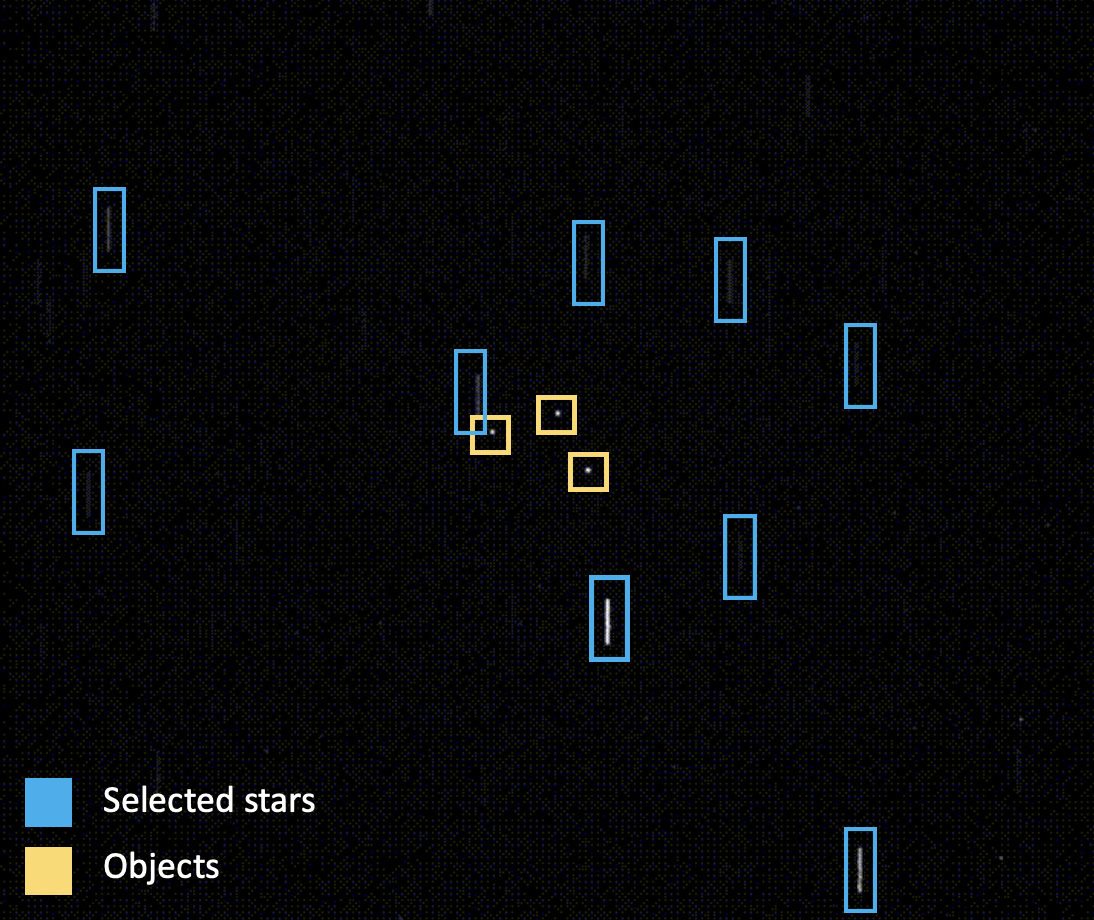
\includegraphics[width=\figmed]{static_images/static_pogs_annotated.png}
  \caption{Raw image of three GEO objects with stars streaking through the background. As expected, the star signals have a variety of signal-to-noise ratios. Taken by the Purdue Optical Ground station at \pogslla by Nathan Houtz.}
  \label{fig:pogs_observation_example}
\end{figure}

Krag \cite{krag2003} modeled this signal by building a $1^\circ \times 1^\circ$ grid of surface
brightness values for the full inertial sphere, parameterized by RA/Dec. Krag used the
Guide Star catalog, which contains 15 million stars down to apparent magnitude 16. Exponential extrapolation
was used to predict star counts in each bin for higher magnitudes \cite{krag2003}. Twenty years later, larger star catalogs exist that are nearly complete to much higher apparent magnitudes. The integrated
starlight catalog used in this work was built from the GAIA catalog with approximately 1.5 billion
stars down to magnitude 21-22 \cite{gaia_dr3}. The same $1^\circ \times 1^\circ$ grid was computed
using GAIA \cite{astroquery_gaia}, resulting in Figure
\ref{fig:gaiapatched} which shows the computed brightness map in units of $S_{10}$. 

\begin{figure}[ht]
  \centering
  \includegraphics[width=\figbig]{sphx_glr_gaia_patched_catalog_001_2_00x.png}
  \caption{Integrated starlight brightness map, produced from Gaia DR3 data \cite{gaia_dr3} using \cite{astroquery_gaia}}
  \label{fig:gaiapatched}
\end{figure}

With this map of exoatmospheric mean brightness of the night sky due to integrated
starlight, the corresponding signal mean in the telescope CCD is computed, adopting Krag's formulation \cite{krag2003}.

\begin{equation} \label{eq:bint}
 \mathcal{Z} = A_\mathrm{aperture}
  \int_{10^{-8}}^{10^{-6}}{ \textrm{STRINT}(\lambda) \cdot \textrm{QE}(\lambda) \cdot \textrm{ATM}(\lambda)
  \cdot \left( \frac{\lambda}{h c} \right) \: d\lambda}  
\end{equation}

In Eq \ref{eq:bint}, $D$ is the telescope aperture diameter in meters, $h$ is Plank's constant in
$\left[ \frac{m^2 kg}{s} \right]$, and $c$
is the speed of light in vacuum in $\left[ \frac{m}{s} \right]$. The resulting quantity
$\mathcal{Z}$ has units of $\left[ \frac{1}{s} \right]$, representing the mean total photons passing
through the telescope aperture due to integrated starlight. 

\begin{equation} \label{eq:starlight_adu}
  \bar{S}_{star} = 10^{-4} \cdot \mathcal{Z} \cdot \left( \frac{s_\mathrm{pix}}{3600} \right)^2 \cdot \Delta t \cdot
  b_{is}
\end{equation}

In Eq \ref{eq:starlight_adu}, $b_{is}$ is the integrated starlight brightness in $\left[ S_{10}
\right]$ computed by linearly interpolating the dataset in Figure \ref{fig:gaiapatched}, $s_\mathrm{pix}$ is the telescope pixel scale in $\left[ \frac{arcsecond}{pix} \right]$ and $\Delta t$ is the integration time in seconds. Note the addition of the $10^{-4}$ factor to reconcile catalog surface brightness in terms of 10th magnitude stars, and the 0th magnitude source in $\mathcal{Z}$. This yields $\bar{S}_{star}$ with units $\left[ \frac{e^-}{pix^2} \right]$; photoelectron counts (ADU) per pixel. Figure \ref{fig:starlight_hemi} shows the background signal mean due to integrated starlight.

\begin{figure}[ht]
  \centering
  \includegraphics[width=\figmed]{sphx_glr_background_signals_002.png}
  \caption{Integrated starlight signal on the local observer hemisphere. The observer is in New Mexico, USA at
  \pogslla}
  \label{fig:starlight_hemi}
\end{figure}

\subsubsection{Scattered Moonlight}

Moonlight scattering through the atmosphere significantly increases background brightness \cite{krag2003}. This scattering effect can be decomposed into Rayleigh (isotropically distributed) and Mie (exponentially distributed) scattering modes. The Rayleigh scattered component is computed with Table 4 published by Daniels parameterized by the angle from the observation to zenith $z_\mathrm{obs}$, the angle from the Moon to zenith $z_\mathrm{Moon}$, and the angle between the observation and the Moon on the horizon $\Delta Az$ \cite{daniels1977}. Interpolating this table yields the intensity of the Rayleigh scattering $F_{rs}$ in $10^{-10}$ $W/(cm^2 \cdot \mu m \cdot sr)$ \cite{krag2003}. The Mie scattered component is formulated \cite{krag2003}:

\begin{equation} \label{eq:mie_scattering_moon}
  F_{ms}(\lambda) = a_1 \left[ e^{-\left(\frac{\Psi}{\Psi_1}\right)} + a_2 e^{-\left(\frac{\pi - \Psi}{\Psi_2}\right)} \right] F_{rs}(\lambda).
\end{equation}

Daniels recommends $a_1 \in [50, 100]$, $a_2 \in [0.01, 0.02]$, $\Psi_1 \in [10^\circ, 20^\circ]$, and $\Psi_2 \approx 50$ \cite{daniels1977}. Prior to any station-specific fitting, the center of each interval is chosen, yielding $a_1 = 75$, $a_2 = 0.015$, $\Psi_1 = 15^\circ$, and $\Psi_2 = 50^\circ$. $a_1$ and $a_2$ are dimensionless, such that $F_{ms}$ also has units of $10^{-10}$ $W/(cm^2 \cdot \mu m \cdot sr)$. The total intensity of the scattered moonlight $F_{mt}$ following Krag's formulation \cite{krag2003}:

\begin{equation} \label{eq:total_scattered_moonlight}
  F_{mt} = f(\theta) \left[ F_{rs}(\lambda) + F_{ms}(\lambda) \right].
\end{equation}

in Eq \ref{eq:total_scattered_moonlight}, $f(\theta)$ is the lunar phase function which describes the fraction of the full Moon brightness reflected at an observer when the Sun-Moon-observer angle is $\theta$. This function is linearly interpolated within Table 3 in \cite{daniels1977}. Finally, Krag introduces a correction factor $f_{corr}$ to account for the difference between the Sun's irradiance spectrum and the spectrum of scattered moonlight, defined to be \cite{krag2003}:

\begin{equation} \label{eq:krag_f_corr}
  f_{corr} = \frac{I_s}{\textrm{SUN}(550 \: \left[\textrm{nm}\right])}.
\end{equation}

With all these pieces, the mean scattered moonlight signal in ADU per pixel is \cite{krag2003}:

\begin{equation} \label{eq:moonlight_adu}
  \bar{S}_\mathrm{Moon} = F_{mt}(550 \: \left[\textrm{nm}\right]) \cdot \mathcal{S}_\mathrm{int} \cdot \left( \frac{s_\mathrm{pix}}{3600} \right)^2 \cdot \Delta t \cdot f_{corr}.
\end{equation}

\begin{figure}[ht]
  \centering
  \includegraphics[width=\figmed]{sphx_glr_background_signals_001.png}
  \caption{Mean scattered moonlight signal on the local observer hemisphere. The observer is in New Mexico, USA at
  \pogslla}
  \label{fig:moonlight_hemi}
\end{figure}

\subsubsection{Zodiacal Light}

Zodiacal light is an effect created by sunlight reflecting off of dust in the ecliptic plane \cite{krag2003}. Zodiacal light is strongest around the Sun --- an exclusion zone for most optical telescopes --- but also reaches a peak directly away from the Sun due to the opposition effect. This peak is known as the Gegenschein, meaning "opposing light". The zodiacal light brightness is linearly interpolated within Table 1 of \cite{roach1972} which is listed for convenience in Appendix \ref{data:roach_zod}. This reports the surface brightness of the zodiacal light $B_\mathrm{zod}(\alpha, \delta)$ in $S_{10}$, which is used without conversion to find the mean CCD signal in ADU per pixel via:

\begin{equation} \label{eq:zodiacal_adu}
  \bar{S}_{zod} = \mathcal{Z} \cdot \left( \frac{s_\mathrm{pix}}{3600} \right)^2 \cdot \Delta t \cdot B_\mathrm{zod}(\alpha, \delta) \cdot 10^{-4}.
\end{equation}

As in the integrated starlight signal, the $10^{-4}$ factor reconciles the $S_{10}$ surface brightness with the 0th magnitude source in $\mathcal{Z}$. 

\begin{figure}[ht]
  \centering
  \includegraphics[width=\figmed]{sphx_glr_background_signals_004.png}
  \caption{Mean zodiacal light signal on the local observer hemisphere. The observer is in New Mexico, USA at
  \pogslla}
  \label{fig:zod_hemi}
\end{figure}

\subsubsection{Background Sampling}

The background signals are only defined in terms of their means, as each signal models the expected amount of radiation without accounting for the quantized nature of light \cite{krag2003}. Since light is transmitted in individual photons, their incidence on a given pixel will follow a statistical distribution. Assuming that each photon does not interact with others, the incidence of a photon on a pixel is well modeled as a Poisson process for each background term \cite{frueh2019notes}. This distribution models the number of independent and identically distributed events that occur during a time period. For CCD astronomy, this translates to the event of a photon hitting the sensor. A Poisson distribution is defined on the positive integers by a single parameter $\lambda$ which is both the mean and variance of the distribution. The probability density function (PDF) for the Poisson distribution takes the form \cite{frueh2019notes}:

\begin{equation} \label{eq:poisson_pdf}
  P_\lambda(x=k) = \frac{\lambda^k e^{-\lambda}}{k!}.
\end{equation}

This distribution has a useful property that $P_{\lambda_1 + \lambda_2}(x=k) = P_{\lambda_1}(x=k) + P_{\lambda_2}(x=k)$ so long as the distributions described by $\lambda_1$ and $\lambda_2$ are independent. The background sources modeled in this work are reasonably assumed to be independent as they each originate from distinct physical processes.

\begin{equation} \label{eq:background_poisson}
  \lambda_\mathrm{background} = \bar{S}_{airglow} + \bar{S}_{pollution} + \bar{S}_{twilight} + \bar{S}_{star} + \bar{S}_\mathrm{Moon} + \bar{S}_{zod}
\end{equation}

Drawing samples from the Poisson distribution defined by $\lambda_\mathrm{background}$ computes the background of the CCD image. 

\subsection{Sensor Effects}

CCD sensors accumulate noise during both the integration time and readout phases. Characterizing these noise sources is necessary to sample realistic light curves and compute the signal-to-noise ratio of the measurements.

\subsubsection{Dark Noise}

The dark noise, also called the dark current or dark count, captures the temperature-dependent accumulation of electrons in the CCD pixel wells \cite{krag2003}. This noise source is modeled as a Poisson process with parameter $\lambda_{dark}$ \cite{frueh2019notes} and is assumed to be independent from the other sensor effects. This source accumulates with the integration time, giving it units of counts per second \cite{krag2003}.

\subsubsection{Readout Noise}

When the CCD is read out, the charge contained in each pixel well must be digitized. This process introduces noise in the final signal due to electronic effects within the CCD circuitry and its surrounding environment \cite{krag2003}. The readout noise is modeled as a zero-mean Gaussian distribution with variance $\sigma_\mathrm{read}^2$ and is also assumed to be independent from other sensor effects \cite{frueh2019notes}.

\subsubsection{Truncation Noise}

Truncation noise in a CCD stems from the fact that the charge in each pixel is digitized into an integer factor of the gain \cite{frueh2019notes}. This is modeled using a uniform distribution on $\left[ -g/2, g/2 \right]$, yielding a variance $N^2_\mathrm{trunc} = \frac{g^2}{24}$ \cite{frueh2019notes}.

The particular noise variances for the Purdue Optical Ground Station are listed in \ref{tb:pogs_parameters}.

\subsection{Observer Constraints}

Accurately simulating light curves requires realistic constraints on the observing station. For an optical ground station, basic operational constraints include local eclipse, target SNR, Moon exclusion angle, and minimum elevation constraints. This section develops these constraints.

\subsubsection{Earth Penumbra}

The Earth casts a conical shadow into space. Outside this shadow, the fraction of received solar irradiance $f_{Sun}$ is assumed to be $1$. Inside the shadow, the central region of zero received solar irradiance $f_{Sun}=0$ is known as umbra, while the boundary between umbra and full Sun is known as the penumbra where $f_{Sun} \in (0,1)$. The precise gradient of the penumbra is defined by the geometry of the overlapping Earth and Sun disks from the perspective of the object. Given the position of the Sun $\vctr{r}_{Sun}$ computed following Section \ref{sec:planet_ephem} and object in J2000, the local irradiance fraction is expressed \cite{krag2003}:

\begin{align*} \numberthis \label{eq:irradiance_fraction_angles}
  \vctr{r}_{obj2Sun} &= \vctr{r}_{Sun} - \vctr{r}_\mathrm{obj} \\
  \epsilon_s &= \sin^{-1}\left( \frac{R_{Sun}}{\| \vctr{r}_{obj2Sun} \|} \right) \\
  \epsilon_e &= \sin^{-1}\left( \frac{R_\mathrm{Earth}(\phi_\mathrm{obj})}{\| \vctr{r}_\mathrm{obj} \|} \right) \\
  \epsilon &= \cos^{-1} \left( -\hat{r}_{obj2Sun} \cdot \hat{r}_\mathrm{obj} \right) \\
  \epsilon_1 &= \frac{\epsilon^2 - \epsilon_e^2 + \epsilon_s^2}{2 \epsilon} \\
  \epsilon_2 &= \frac{\epsilon^2 + \epsilon_e^2 - \epsilon_s^2}{2 \epsilon}. \\
\end{align*}

\graphicspath{{/Users/liamrobinson/Documents/msthesis/static_images}}
\begin{figure}[!htb]
  \centering
  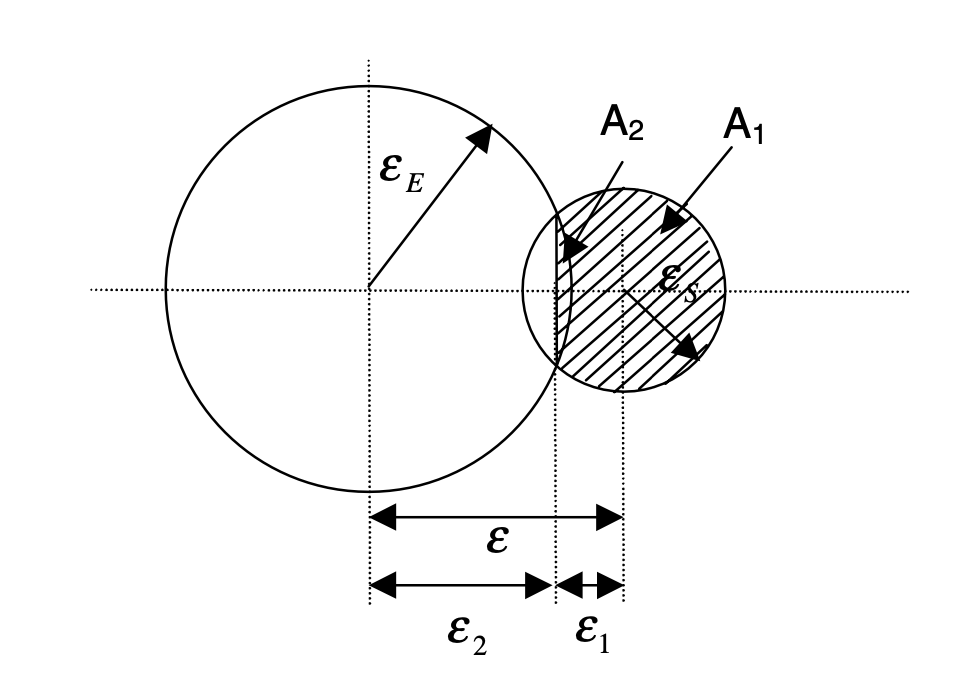
\includegraphics[width=\figmed]{angle_defs_krag_520.png}
  \caption{Angle and area definitions for penumbra shadowing, Figure 5.20 in \cite{krag2003}}
  \label{fig:penumbra_angles}
\end{figure}
\graphicspath{{/Users/liamrobinson/Documents/msthesis/static_images/aas_2022_figs}}

In Eq \ref{eq:irradiance_fraction_angles}, $\epsilon_s$ is the half-angle of the Sun disk at the object, $\epsilon_e$ is the half-angle of the Earth disk from the object as a function of the geodetic latitude of the object $\phi_\mathrm{obj}$. Additionally, $\epsilon$ is the angle between the center of the Earth and Sun from the perspective of the object, with $\epsilon_1$ and $\epsilon_2$ being the angles from the center of the Sun and Earth disks to the center of their overlap, if it exists \cite{krag2003}. These angles are defined in Figure \ref{fig:penumbra_angles}. Given these angles, the illumination fraction $f_{Sun}$ is computed:

\begin{equation} \label{eq:irradiance_fraction}
  f_{Sun} = \begin{cases}
    1 & \epsilon \geq (\epsilon_s + \epsilon_e) \\ 
    0 & \epsilon \leq (\epsilon_e - \epsilon_s) \\ 
    \frac{a_1 - a_2}{\pi \epsilon_s^2} & \mathrm{else}
  \end{cases}.
\end{equation}

In Eq \ref{eq:irradiance_fraction}, the solid angles $a_1$ and $a_2$ are defined in Figure \ref{fig:penumbra_angles} and are computed via:

\begin{align*} \numberthis \label{eq:penumbra_areas}
  a_1 &= \pi \epsilon_s^2 - \epsilon_s^2 \cos^{-1} \left(\frac{\epsilon_1}{\epsilon_s}\right)
    + \epsilon_1 \sqrt{\epsilon_s^2 - \epsilon_1^2} \\
  a_2 &= \epsilon_e^2 \cos^{-1}\left(\frac{\epsilon_2}{\epsilon_e} \right) - \epsilon_2 \sqrt{\epsilon_e^2 - \epsilon_2^2} \\
\end{align*}

Computing Eq \ref{eq:irradiance_fraction} for a dense grid of points in the J2000 reference frame reveals the geometry of the penumbra and umbra in Figure \ref{fig:penumbra}, illustrating that the penumbra expands into the umbra as the observer recedes from the Earth. 

\graphicspath{{/Users/liamrobinson/Documents/PyLightCurves/docs/build/html/_images}}
\begin{figure}[!htb]
  \centering
  \includegraphics[width=\figbig]{sphx_glr_penumbra_plane_001.png}
  \caption{Shadow fraction in J2000, effect exaggerated by scaling the Sun radius by a factor $10$}
  \label{fig:penumbra}
\end{figure}
\graphicspath{{/Users/liamrobinson/Documents/msthesis/static_images/aas_2022_figs}}

\subsubsection{SNR}

As the signal-to-noise ratio of an object signal on the CCD pixel grid degrades, it becomes more difficult to determine whether an object is present at all. Given a minimum limiting SNR $\mathrm{SNR}_{min}$ this constraint takes the form:

\begin{equation} \label{eq:snr_exclusion}
  \nu_{\mathrm{SNR}} = \begin{cases}
    1 & \mathrm{SNR} > \mathrm{SNR}_{min}\\
    0 & \mathrm{else}
  \end{cases}.
\end{equation}

In Eq \ref{eq:snr_exclusion}, $\nu_{\mathrm{SNR}} = 1$ implies that the observation is valid, with $\nu_{\mathrm{SNR}} = 0$ implying that the object signal cannot be discerned from the image background.

\subsubsection{Moon Exclusion Angle}

Focusing the irradiance of the Moon onto the sensor grid will seriously damage the CCD. For the Purdue Optical Ground Station, stray light from the Moon begins leaking into the optics around $30^\circ$ from the center of the Moon disk. This observation constraint is imposed for an arbitrary exclusion angle $\theta_{Moon,ex}$ via:

\begin{equation} \label{eq:moon_exclusion}
  \nu_\mathrm{Moon} = \begin{cases}
    1 & \cos^{-1}\left( \frac{\left( \vctr{r}_\mathrm{Moon} - \vctr{r}_\mathrm{obs} \right) \cdot \left( \vctr{r}_\mathrm{obj} - \vctr{r}_\mathrm{obs} \right)}{\| \vctr{r}_\mathrm{Moon} - \vctr{r}_\mathrm{obs} \| \| \vctr{r}_\mathrm{obj} - \vctr{r}_\mathrm{obs} \|} \right) > \theta_{Moon,ex}\\
    0 & \mathrm{else}
  \end{cases}.
\end{equation}

In Eq \ref{eq:moon_exclusion}, $\nu_\mathrm{Moon} = 1$ implies that the observation is valid, with $\nu_\mathrm{Moon} = 0$ implying that the observation is too close to the Moon. $\vctr{r}_\mathrm{Moon}$ should be computed with SPICE following Section \ref{sec:planet_ephem}.

\subsubsection{Minimum Elevation}

Due to the local topology at the observer location, an operator may assign a minimum angle from the horizon $\theta_{elev,min}$ for observations. Approximating the station inertial position $\vctr{r}_\mathrm{obs}$ as being aligned with zenith, this yields the condition:


\begin{equation} \label{eq:elevation_exclusion}
  \nu_{elevation} = \begin{cases}
    1 & 90^\circ - \cos^{-1}\left( \frac{\left( \vctr{r}_\mathrm{obj} - \vctr{r}_\mathrm{obs} \right) \cdot \left( \vctr{r}_\mathrm{obs} \right)}{\| \vctr{r}_\mathrm{Moon} - \vctr{r}_\mathrm{obs} \| \| \vctr{r}_\mathrm{obs} \|} \right) > \theta_{elev,min}\\
    0 & \mathrm{else}
  \end{cases}.
\end{equation}

In Eq \ref{eq:elevation_exclusion}, $\nu_{elevation} = 1$ implies that the observation is valid, with $\nu_{elevation} = 0$ implying that the observation is too close to the horizon.

\subsection{Mean Irradiance at The Observer}

Given the normalized irradiance computed via Eq \ref{eq:lc_func_normalized} for convex objects or Eq \ref{eq:lc_normalized_engine} for any object shaded using Algorithm \ref{alg:pix_shading}, the received mean irradiance at the telescope aperture is given by:

\begin{equation} \label{eq:mean_irrad_at_aperture}
  \bar{I} = \nu_{Moon,ex} \cdot \nu_{elevation} \cdot \nu_{\mathrm{SNR}} \frac{I_s f_{Sun} \hat{I}}{\left( \vctr{r}_\mathrm{obj} - \vctr{r}_\mathrm{obs} \right)^2}.
\end{equation}

In Eq \ref{eq:mean_irrad_at_aperture}, the conditions $\nu_{Moon,ex},\: \nu_{elevation},\: \nu_{\mathrm{SNR}}$ determine whether the telescope can take the observation and identify the object in the image, $I_s f_{Sun}$ determines the solar irradiance incident on the object, and the remaining terms $\hat{I} / \left( \vctr{r}_\mathrm{obj} - \vctr{r}_\mathrm{obs} \right)^2$ dimensionalize the normalized irradiance. In order to sample a noisy light curve, this mean irradiance must be converted into a mean photoelectron count via Eq \ref{eq:irrad_to_count}, yielding $\bar{C}_\mathrm{all}$:

\begin{equation}
  \bar{C}_\mathrm{all} = \mathcal{S}_\mathrm{int} \cdot \bar{I} \cdot \Delta t.
\end{equation}

\subsection{Sampling Noisy Light Curves} \label{sec:sampling_lcs}

Given the irradiance of the object observed by the telescope, the noisy light curve is computed by building a grid containing the object signal, background noise, and sensor noise. On a pixel-by-pixel basis, the mean object signal is given by an alteration of Eq \ref{eq:airy_gaussian} where the angle $\theta$ from the center of the frame is converted into pixels via $\theta^2 = \left((x - x_0)^2 + (y - y_0)^2 \right) / s_\mathrm{pix}^2$:

\begin{equation} \label{eq:obj_signal_grid}
  \bar{C}_\mathrm{obj}(x, y) = \frac{0.838 \bar{C}_\mathrm{all}}{2 \pi \sigma^2} \exp\left( - \frac{(x - x_0)^2 + (y - y_0)^2}{2 \sigma^2  s_\mathrm{pix}^2} \right).
\end{equation}

In Eq \ref{eq:obj_signal_grid}, $\left(x_0, y_0\right)$ are the exact pixel coordinates of the object centroid, $\sigma$ is the Gaussian standard deviation from Eq \ref{eq:airy_variance} in arcseconds, and $s_\mathrm{pix}$ is the pixel scale in arcseconds per pixel. Likewise, the total noise sampled in each pixel is given by samples from all the relevant source distributions:

\begin{equation} \label{eq:noise_signal_grid}
  C_{noise} = N_\mathrm{background} + N_{dark} + N_\mathrm{trunc} + N_\mathrm{read}.
\end{equation}

In Eq \ref{eq:noise_signal_grid}, $N_\mathrm{background}$ is a sample drawn from $\mathrm{Pois}(\lambda_\mathrm{background})$, $N_{dark}$ is drawn from $\mathrm{Pois}(\Delta t \cdot \lambda_{dark})$, $N_\mathrm{trunc}$ is drawn from $\mathrm{Uniform}(-g/2, g/2)$, and $N_\mathrm{read}$ is drawn from $\mathrm{N}(0, \sigma_\mathrm{read}^2)$. 

Assuming perfect knowledge of the image background mean in the region around the object signal --- a reasonable assumption given that there are generally millions of background pixels in the image --- the counts $C_{obj,meas}$ attributed to the object pixels $\{x_\mathrm{obj}, y_\mathrm{obj}\}$ is given by:

\begin{align*} \numberthis \label{eq:noisy_counts}
  C_{noise,all} &= \sum_{i=1}^{A_\mathrm{Airy}}{C_{noise,i}} \\
  C_{obj,all} &= \sum_{x \in x_\mathrm{obj}, \: y \in x_\mathrm{obj}}{\bar{C}_\mathrm{obj}(x, y)} \\
  C_{obj,meas} &= C_{noise,all} - A_\mathrm{Airy} \left( \Delta t \cdot \lambda_{dark} + \lambda_\mathrm{background} \right) 
\end{align*}

In Eq \ref{eq:noisy_counts}, $A_\mathrm{Airy}$ is the area of the central maximum of the Airy disk in square pixels presented in Eq \ref{eq:airy_area}. The measured object signal $C_{obj,meas}$ can then be transformed into irradiance via Eq \ref{eq:count_to_irrad}:

\begin{equation} \label{eq:noisy_counts_to_irrad}
  I_{obj,meas} = \frac{C_{obj,meas}}{\mathrm{\mathcal{S}_\mathrm{int}} \cdot \Delta t}
\end{equation}

or to apparent magnitude by applying Eq \ref{eq:mag_to_irradiance}:

\begin{equation}
  m_{obj,meas} = -2.5 \log_{10}\left( \frac{I_{obj,meas}}{I_0} \right)
\end{equation}

or normalized irradiance by applying Eq \ref{eq:irradiance_to_norm_irradiance}:

\begin{equation} \label{eq:ihat_meas}
  \hat{I}_{obj,meas} = \frac{\| \vctr{r}_\mathrm{obj} - \vctr{r}_\mathrm{obs} \|^2}{I_s} I_{obj,meas}.
\end{equation}

\section{Light Curve Simulation Results}

\subsection{Case 1: Normalized Light Curve of a Simple Object}

This section presents the entire process for simulating the normalized light curve of a simple object. To begin, the properties of the object and the observing station are defined in Table \ref{tb:case1_obj_props}. The cube model used for this case is displayed in Figure \ref{fig:case1_obj}.

\begin{table}[]
  \centering
  \begin{tabular}{|l|l|}
  \hline
  \textbf{Parameter} & \textbf{Value} \\ \hline
  Object & \texttt{cube.obj} \ref{sec:obj_listing} \\ \hline
  SATNUM & $36411$ \\ \hline
  $q_0$ & $\left[ 0, 0, 0, 1 \right]^T$ \\ \hline
  $w_0$ & $\left[ 0.04082483, 0.08164966, 0.04082483 \right]^T$ $[rad/s]$ \\ \hline
  $J$ & $\mathrm{diag}\left( 1.0, 2.0, 3.0 \right)$ $\left[ kg \cdot m^2 \right]$ \\ \hline
  BRDF & Phong \\ \hline
  $C_s$ & $0.3$ \\ \hline
  $C_d$ & $0.7$ \\ \hline
  $n$ & $5$ \\ \hline
  Initial date & 2023-03-26 05:00:00 UTC \\ \hline
  $\Delta t$ & $0.1$ $[s]$ \\ \hline
  $n_\mathrm{obs}$ & $360$ $[s]$ \\ \hline
  $\phi_{geod}$ & $32.900^\circ$ \\ \hline
  $\lambda$ & $-105.533^\circ$ \\ \hline
  \end{tabular}
  \caption{Object and station simulation parameters for case 1}
  \label{tb:case1_obj_props}
\end{table}

\graphicspath{{/Users/liamrobinson/Documents/PyLightCurves/docs/build/html/_images}}
\begin{figure}[!htb]
  \centering
  \includegraphics[width=\figmed]{sphx_glr_light_curves_types_001.png}
  \caption{Cube model for case 1}
  \label{fig:case1_obj}
\end{figure}

To begin, the position of the object in TEME is computed using SGP4. That position is converted to ICRF using Eqs \ref{eq:teme_to_tod}, \ref{eq:tod_to_mod}, and \ref{eq:mod_to_icrf}. The position of the station in ITRF is computed using Eq \ref{eq:lla_to_itrf} and converted to ICRF using Eqs \ref{eq:itrf_to_gtod}, \ref{eq:gtod_to_teme}, \ref{eq:teme_to_tod}, \ref{eq:tod_to_mod}, and \ref{eq:mod_to_icrf}. The position of the Sun is determined with SPICE following Section \ref{sec:planet_ephem}. 

The attitude profile of the object is propagated with Eqs \ref{eq:rbtf_dynamics} and \ref{eq:quat_kde} using $\vctr{M}=\mathbf{0}$ for torque free rigid body motion. The resulting attitude time history produces $q(t)$, $\omega(t)$, as well as the body frame vectors from the object to the Sun and observer depicted in Figure \ref{fig:case1_attitude}.

\begin{figure}[!htb]
  \centering
  \includegraphics[width=\textwidth]{sphx_glr_light_curves_types_002_2_00x.png}
  \caption{Attitude time history for case 1}
  \label{fig:case1_attitude}
\end{figure}

Next, the BRDF is used to compute the reflection matrix for the cube with Eq \ref{eq:reflection_matrix}. The normalized light curve is simply computed with Eq \ref{eq:lc_func_normalized}, using Eq \ref{eq:brdf_phong} and noting that $\mu_{ij} = 0$ as the object is convex. This yields the normalized light curve depicted in Figure \ref{fig:case1_lc}.

\begin{figure}[!htb]
  \centering
  \includegraphics[width=\figmed]{sphx_glr_light_curves_types_004_2_00x.png}
  \caption{Normalized light curve for case 1}
  \label{fig:case1_lc}
\end{figure}

Figure \ref{fig:case1_lc} has a few important features to recognize. Some sections of the light curve are flat, indicating that all illuminated faces are orthogonal to each other and reflecting diffusely. When one of the face normal vectors approaches the halfway vector $H$, a specular glint occurs, leading to a temporary sharp increase in the light curve value. Overall, this is exactly the behavior expected given the observation conditions.

\subsection{Accurate Satellite Models}

To produce accurate light curves for real space objects, 3D model files were collected and tuned for use with the light curve simulator. These models are shown in Figure \ref{fig:satellite_lineup}. Each model is correctly scaled, with accurate material properties applied to their faces. Figure \ref{fig:satellite_lineup} highlights the size of the GEO communications satellites (TELSTAR, HYLAS, Hispasat, and ASTRA). In contrast, the LEO satellites (Starlink and Landsat) are dwarfed at the left end of the lineup.

\begin{figure}[ht]
    \centering
    \includegraphics[width=\figbig]{sphx_glr_satellite_lineup_001.png}
    \caption{Selected space objects with soccer field for size reference. In order, the objects are TESS, Starlink V1, TDRS, Landsat 8, Hispasat 30W-6, Saturn V SII, TELSTAR 19V, HYLAS 4, and simplified ASTRA.
    }
    \label{fig:satellite_lineup}
\end{figure}

\subsection{Case 2: Realistic Light Curve for a Box-Wing Satellite} \label{sec:case2}

The second case deals with simulating a realistic noisy light curve for a complex, nonconvex satellite model with observer constraints. Table \ref{tb:case2_obj_props} summarizes the simulation parameters for the object and station. The object geometry is displayed in Figure \ref{fig:case2_obj}.

\begin{table}[]
  \centering
  \begin{tabular}{|l|l|}
  \hline
  \textbf{Parameter} & \textbf{Value} \\ \hline
  Object & \href{https://raw.githubusercontent.com/liamrobinson1/Light-Curve-Models/main/accurate_sats/matlib_goes17.obj}{goes17.obj} \\ \hline
  SATNUM & $32711$ \\ \hline
  $q_0$ & $\left[ 0, 0, 0, 1 \right]^T$ \\ \hline
  $w_0$ & $\left[ 0.00707107, 0.,         0.00707107 \right]^T$ $[rad/s]$ \\ \hline
  $J$ & $\mathrm{diag}\left( 1.0, 2.0, 2.0 \right)$ $\left[ kg \cdot m^2 \right]$ \\ \hline
  BRDF & Phong \\ \hline
  Initial date & 2022-12-09 08:00:00 UTC \\ \hline
  $\Delta t$ & $10$ $[s]$ \\ \hline
  $n_\mathrm{obs}$ & $180$ $[s]$ \\ \hline
  Telescope & Table \ref{tb:pogs_parameters} \\ \hline
  $\phi_{geod}$ & $32.900^\circ$ \\ \hline
  $\lambda$ & $-105.533^\circ$ \\ \hline
  $SNR_{min}$ & $3$ \\ \hline
  $\theta_{Moon,ex}$ & $30^\circ$ \\ \hline
  $\theta_{elev,min}$ & $15^\circ$ \\ \hline
  \end{tabular}
  \caption{Object and station simulation parameters for case 2}
  \label{tb:case2_obj_props}
\end{table}

\begin{figure}[!htb]
  \centering
  \includegraphics[width=\figmed]{sphx_glr_light_curves_types_005.png}
  \caption{GOES 17 model for case 2}
  \label{fig:case2_obj}
\end{figure}

To begin, the position of the object in TEME is computed using SGP4. That position is converted to ICRF using Eqs \ref{eq:teme_to_tod}, \ref{eq:tod_to_mod}, and \ref{eq:mod_to_icrf}. The position of the station in ITRF is computed using Eq \ref{eq:lla_to_itrf} and converted to ICRF using Eqs \ref{eq:itrf_to_gtod}, \ref{eq:gtod_to_teme}, \ref{eq:teme_to_tod}, \ref{eq:tod_to_mod}, and \ref{eq:mod_to_icrf}. The position of the Sun is determined with SPICE following Section \ref{sec:planet_ephem}. 

The attitude profile of the object is propagated with Eqs \ref{eq:rbtf_dynamics} and \ref{eq:quat_kde} using $\vctr{M}=\mathbf{0}$ for torque free rigid body motion. The resulting attitude time history produces $q(t)$, $\omega(t)$, as well as the body frame vectors from the object to the Sun and observer depicted in Figure \ref{fig:case2_attitude}.

\begin{figure}[!htb]
  \centering
  \includegraphics[width=\textwidth]{sphx_glr_light_curves_types_006_2_00x.png}
  \caption{Attitude time history for case 2}
  \label{fig:case2_attitude}
\end{figure}

The BRDF --- which varies across the surface of the object --- is encoded in the \texttt{.obj} file in the red channel of the diffuse material color $R$ such that $C_d = R$ and $C_s = 1 - R$. Given the unit vectors in the object body frame pointing towards the observer and the Sun, Algorithms \ref{alg:depth_map} and \ref{alg:pix_shading} are used to render images of the object which are integrated to yield a mean normalized irradiance value $\hat{I}$ with Eqs \ref{eq:ortho_area} and \ref{eq:lc_normalized_engine}. 

This normalized irradiance is dimensionalized with Eq \ref{eq:irradiance_to_norm_irradiance} to yield a mean irradiance $I$. Next, the background signal variances are computed for the Moonlight in Eq \ref{eq:moonlight_adu}, zodiacal light in Eq \ref{eq:zodiacal_adu}, integrated starlight in Eq \ref{eq:starlight_adu}, twilight in eq \ref{eq:twilight_adu}, light pollution in Eq \ref{eq:pollution_adu}, and airglow in Eq \ref{eq:airglow_adu}. These background signal variances are used to compute the overall background variance $\lambda_\mathrm{background}$. The signal variance due to read noise, dark noise, and truncation noise are found in Table \ref{tb:pogs_parameters}, yielding the overall mean and variance of the background pixels. 

These means and variances are used to compute the SNR of each attempted observation using Eq \ref{eq:ccd_snr}. This SNR is used compute the minimum SNR constraint in Eq \ref{eq:snr_exclusion}. The Moon exclusion angle constraint is also evaluated with Eq \ref{eq:moon_exclusion} and the minimum elevation constraint is evaluated with Eq \ref{eq:elevation_exclusion}. If all constraints are satisfied, the object is observable and the light curve measurement process can continue. Otherwise, the measurement is impossible and no value is saved for this timestep.

The mean value of the total photoelectron counts due to the object signal is computed from the mean irradiance $I$ using Eq \ref{eq:irrad_to_count} using the telescope parameters in Table \ref{tb:pogs_parameters}. This total mean count is then distributed across the CCD pixel grid using Eq \ref{eq:obj_signal_grid}. Now that all mean values are known, samples from the Poisson, Gaussian, and uniform distributions are sampled pixel-by-pixel to yield a final background and object signal on the CCD grid. The noisy light curve in ADU is then computed with Eq \ref{eq:noisy_counts} and transformed back to irradiance with Eq \ref{eq:noisy_counts_to_irrad}, depicted in Figure \ref{fig:case2_lc}.

\begin{figure}[!htb]
  \centering
  \includegraphics[width=\figmed]{sphx_glr_light_curves_types_007_2_00x.png}
  \caption{Light curve for case 2, produced with an object scale factor of $1/10$ to exaggerate noise}
  \label{fig:case2_lc}
\end{figure}

Figure \ref{fig:case2_lc} possesses a few important characteristics to note when compared to the results from case 1 in Figure \ref{fig:case1_lc}. The light curve for case 2 is much more complex, with higher frequency variation in the mean due to the many small geometric features making up the satellite model. As in the cube light curve, specular peaks are still evident around $260$ and $1050$ seconds after the simulation epoch. The noise is clearly seen in the regions shaded by standard deviation. As a result of this noise, the lower magnitude signals regions --- where little specular reflection is occurring --- are much more corrupted by the noise as its standard deviation represents a larger fraction of the signal magnitude. Importantly, these regions possess high-frequency oscillations in the mean that are highly obscured in any one sampling due to the additive noise. This highlights the importance of specular reflection for extracting reliable accurate features by pinpointing the normal vectors of certain faces by reaching above the noise. It must be noted that Figure \ref{fig:case2_lc} was produced with a scale factor of $1/10$ applied to the vertices of the GOES 17 3D model to make the effect of the noise more clear. In reality, large GEO objects like GOES should produce light curves with much less noise on the signal, as predicted by the simulator developed in this work. 
\ProvidesFile{ch-light-curve-inversion.tex}[Light Curve Shape Inversion]
\graphicspath{{/Users/liamrobinson/Documents/PyLightCurves/docs/build/html/_images}}
\chapter{Light Curve Shape Inversion}

\section{Nature of The Problem}

The problem of light curve shape inversion is plagued by different types of ambiguities. In order to understand the later inversion methods, it is important to understand the characteristics of each ambiguity.

\subsection{Ambiguities}

Many types of ambiguities exist in the light curve shape inversion problem. Some of these ambiguities can be resolved or reduced by collecting more light curve data, but others are inherent to the problem and remain regardless of the quality or quantity of available data.

\subsubsection{Albedo-Area}

The interplay between the coefficients of reflection of the object's surfaces and their areas creates an ambiguity in the final estimated shape \cite{fan2020thesis}. These factors are considered together as the \textit{albedo-area}. For a given shape, there exist an infinite family of geometrically similar shapes which possess the same albedo area with face areas scaled by a nonzero scalar $c$ and coefficients of reflection scaled by $c^{-1}$, constrained such that the scaled face albedo cannot violate energy conservation \cite{fan2020thesis}. This behavior is displayed in Figure \ref{fig:albedo_amb}.

\begin{figure}[!htb]
  \centering
  \includegraphics[width=\figmed]{sphx_glr_light_curve_ambiguities_001_2_00x.png}
  \caption{Albedo-area ambiguity for a cube in an arbitrary torque-free rigid body attitude profile illuminated using a Cook-Torrance BRDF}
  \label{fig:albedo_amb}
\end{figure}

Further ambiguities lie in the albedo-area variations of subsets of the object geometry. For example, scaling the areas of the end caps of a cylinder has the same effect on the light curve as applying the same scaling to their albedo. These families produce the same light curve in the same observation conditions, and thus no decision can be made about the object's true scale within without additional information \cite{fan2020thesis}.

\subsubsection{Orientation}

Multiple orientations of the object may produce the same light curve value \cite{burton2023attitude}. This behavior is demonstrated for a cube in Figure \ref{fig:brightness_iso}, where the continuous surfaces in attitude space sharing a common brightness value are plotted. 

\begin{figure}[!htb]
  \centering
  \includegraphics[width=\figmed]{sphx_glr_light_curve_iso_surfaces_002.png}
  \caption{Brightness isosurfaces in rotation vector $\vctr{p} = \theta \hat{\lambda}$ for a cube with face areas $a_i = 4$ illuminated using a Phong BRDF with $C_d=0.5$, $C_s=0.5$, $n=5$ at $\phi=45^\circ$ and normalized irradiance value $\check{I} = 0.73$}
  \label{fig:brightness_iso}
\end{figure}

Figure \ref{fig:brightness_iso} points to a more general conclusion about the coupling of the light curve and object orientation. Even if the shape of the object is known precisely, a single light curve measurement is not sufficient to determine the object's attitude due to this coupling.

\subsubsection{Object Symmetry}

Objects with symmetries in their albedo-area are also ambiguous in the shape inversion problem. This follows from common sense: the shape and attitude of a cylinder with a uniform BRDF can only be determined up to a rotation about the axis of symmetry. Any particular value chosen for that rotation would be have to be arbitrary and cannot be driven by the data in the light curve alone. Likewise, a uniformly reflecting cube's shape and orientation is determined only up to any combination of $90^\circ$ rotations about the axes of symmetry. Thankfully, these ambinguities due to symmetry often have no impact on the usefulness of the inverted result as by definition they represent geometrically identical objects.

\subsubsection{Observation Geometry}

If the directions of the Sun and observer in the body frame of the object are swapped --- thereby rotating the object about the Sun-object-observer bisector vector by $180^\circ$ --- the light curve will be identical if the body has the same initial angular velocity \cite{burton2023attitude}. This equivalence holds so long as the phase angle of the observation is the same \cite{burton2023attitude}. This follows from the reciprocity of light reflection as modeled by the BRDF as well as the reciprocity of the shadows \cite{burton2023attitude}. Upon rotating the object as described, areas which were previously Sun-shadowed become observer-shadowed and vice versa, preserving the total amount of shadowing and therefore the overall light curve. Figure \ref{fig:obs_amg} displays this behavior.

\begin{figure}[!htb]
  \centering
  \includegraphics[width=\figmed]{sphx_glr_light_curve_ambiguities_002_2_00x.png}
  \caption{Obseravtion geometry ambiguity for a cube in an arbitrary rigid body attitude profile.}
  \label{fig:obs_amg}
\end{figure}

In the context of shape inversion, this behavior yields two equally plausible solutions for the object's shape in a given attitude profile that are offset from eachother by a rigid rotation of $180^\circ$ in the body frame \cite{burton2023attitude}. 

\subsubsection{Nonconvex Shape Features}

The influence of concavities are only observable in the light curve due to the variability of self-shadowing \cite{durech2003}. Sometimes, certain faces of an object with concavities may be fully illuminated while at other times those faces may have shadows cast on them due to other parts of the object geometry. The larger the phase angle $\phi$ between the Sun and observer directions, the more self-shadowing will take place until no faces can be illuminated and viewed simultaneously at $\phi=180^\circ$ \cite{durech2003}.

If a concave feature does contribute to the light curve while self-shadowing is occurring, new ambiguities are introduced. A single concave feature can be broken up into multiple smaller concavities with the same interior geometry and proportionally smaller face areas \cite{durech2003}. Similarly, other concavity geometries may produce the same aggregate effect on the light curve \cite{durech2003}. This particular ambiguity is truly unresolvable due to the unobservability of the face connectivity --- and more generally the final construction of the object --- from the light curve alone, as discussed in Section \ref{sec:full_shape}.

\subsection{Face Observability}

Depending on the object attitude profile and the geometry of the observer and the Sun, some faces of the object may never be illuminated and observed at the same time \cite{fan2020thesis}. In such cases, no information is available to constrain the geometry of these unilluminated, unobserved faces. As an example, a cylinder rotating about its axis of symmetry may never point an end face towards the observer over a set of observations. Without any information on these faces, the hidden geometry within that region is unknown and the shape estimate is ambiguous. This ambiguity can be resolved by waiting until the observation geometry and object orientation change to allow these regions of the object to be illuminated and observed \cite{friedman2020}. 

% If an object is viewed at a constant phase angle of $\phi = 0^\circ$ between the Sun and observer vectors, no self-shadowing can occur and the resulting light curve will be well-fit by a convex estimate \cite{durech2003}. Similarly, a concavity that is never illuminated or is never able to be observed while illuminated is unobservable as its self-shadowing effects are not present in the observed light curve \cite{durech2003}.

\subsection{Full Shape Observability} \label{sec:full_shapes}

Although the light curve contains information that aids in shape estimation, the particular construction of the object is fundamentally unobservable, independent of object convexity \textit{I really need a citation here, but I cannot find any paper that makes this point about the inversion problem in general}. Every shape inversion method makes an assumption about how the object shape may be constructed from the information in the light curve. For example, EGI-based methods construct a convex approximation of the geometry by leveraging the Minkowski problem while filter-based methods may assume that the object is one of a set of known shapes. These assumptions are not driven by the data, as the data fundamentally cannot reveal the construction of the object without ambiguity.

\subsubsection{Bayesian Inversion Implications}

It would be advantageous is Bayes' theorem could be easily applied to iteratively update a shape estimate as measurements are collected. Many iterative shape and attitude inversion methods already do this, applying Bayes' theorem to compute the probability of a given shape hypothesis $M^\ell$ for a set of light curve measurements $I_{1:i}$, via \cite{linares2018space}:

\begin{equation}
  P(M^\ell \vert I_{1:i}) = \frac{P(I_{1:i} \vert M^\ell)P(M^\ell)}{P(I_{1:i})}.
\end{equation}

Linares and Crassidis note that in most cases, computing the normalizing factor $P(I_{1:i})$ is not tractable as it is equivalent to integrating over the space of possible shapes \cite{linares2018space}:

\begin{equation}
  P(I_{1:i}) = \int P(I_{1:i} \vert M^\ell)P(M^\ell) dM^\ell.
\end{equation}

The filter-based inversion literature proposes various methods for circumventing this issue. Multiple authors have used a Markov Chain Monte Carlo (MCMC) method to remove the need for the normalizing factor while still approaching the target posterior distribution in the limit of the chain \cite{linares2018space, campbell2023}. Linares et al.\ discretize the shape space with a Multiple Model Adaptive Estimation (MMAE) method which approximates the normalizing factor using a bank of $n$ known shape models $M^\ell_j)$ \cite{linares2014space}:

\begin{equation}
  P(I_{1:i}) = \sum_{j=1}^n P(I_{1:i} \vert M^\ell_j)P(M^\ell_j).
\end{equation}

This implicitly assumes that the set of chosen models sufficiently spans the space of possible space object shapes. This assumption is not necessarily true for real observations, where there may be significant uncertainty associated with the object's identity and origin. In such cases, this assumption could cause the MMAE method to become overly confident in a particular shape model in its bank as it has no sense of the space of shapes outside the bank.

As a result, filter-based methods make the same core assumption the direct methods: they assume a construction or selection method to determine the final geometry. Because this non-data-driven step is required to produce a shape estimate, a full Bayes update is not possible for the shape inversion problem and workarounds must be developed in each Bayesian method to approximate the posterior distribution \cite{linares2012, linares2014space, campbell2023, linares2017}.

% In the context of shape inversion, we seek to find the shape $A$ that best explains the light curve $B$. To evaluate the probability of a given shape mesh estimate $\mathcal{M}_i$ based on light curve data $I_{1:i}$, the quantities $P(\mathcal{M}_i)$ and $P(I_{1:i})$ are required. The probability of a given mesh estimate $P(\mathcal{M}_i)$ is difficult to evaluate, as it is not clear how to define a prior distribution over the space of all possible meshes. As a result, it is impractical to perform a full Bayesian update on a given shape estimate.

\graphicspath{{/Users/liamrobinson/Documents/msthesis/static_images/aas_2022_figs}}

\section{Direct Convex Shape Inversion}

Traditionally, direct light curve inversion involves two distinct optimization problems: a linear least squares problem to optimize normal vectors and areas to match the measured light curve, and a second optimization to produce accurate vertex positions and face adjacency information \cite{fan2020thesis, kaasalainen2000, kaas2001shape, cabrera2021}. The first problem is data-driven and linear, using the observations to estimate a plausible EGI. The second problem is highly nonlinear but convex and requires significant tuning for robust convergence \cite{fan2019}. The full convex inversion process presented in this work is outlined:

\begin{outline}[enumerate]
  \1 Area and normal vector optimization
    \2 Initial normal vector sampling
    \2 Initial face area optimization
    \2 Normal vector resampling
    \2 Face area reoptimization
    \2 Face merging
  \1 Object reconstruction
    \2 Face support optimization
    \2 Dual transform yielding final vertex locations
    \2 Convex hull yielding final face adjacency relationships
\end{outline}

\subsection{The Extended Gaussian Image} \label{sec:egi_definition}

In the continuous case, the Gaussian Image associates each point on the surface of a shape with a outward-pointing normal vector direction on the unit sphere $\mathbb{S}^2$ \cite{horn1984}. The determinant of the Jacobian of this forward mapping yields the Gaussian curvature $\kappa(u,v)$ of the surface at each surface point --- expressing how rapidly local normal vectors change direction \cite{horn1984}. The continuous \textit{Extended} Gaussian Image (EGI) $E(\theta, \phi)$ is a function on the unit sphere parameterized by an azimuth $\theta$ and elevation $\phi$ which sums the inverse Gaussian curvature for all points $(u_i, v_i)$ on the surface of the object with a normal pointing towards $(\theta, \phi)$ \cite{horn1984}:

\begin{equation} \label{eq:egi_deg}
  E(\theta, \phi) = \sum_i{\frac{1}{\| \kappa(u_i, v_i) \|}}.
\end{equation}

By Eq \ref{eq:egi_deg}, flat areas of the object are mapped to point masses in the EGI, motivating a simpler definition of the EGI for discrete surfaces. The discrete EGI $\vctr{E} \in \mathbb{R}^{m \times 3}$ is composed of $m$ unit vectors $\vctr{N}$ each scaled by a nonnegative areea $a \in \mathbb{R}$, where $a_i \geq 0 \forall i$ \cite{little1983}.

\begin{equation}
  \vctr{E}_i = a_i \vctr{N}_i
\end{equation}

In the context of shape inversion, the $m$ vectors $\vctr{N}$ should be a relatively uniform tessellation of the unit sphere. A convex polytope can be uniquely represented by an EGI of facet normal vectors scaled by each facet's area. The set of normal vectors in an EGI is denoted $\mathcal{N}$ with the set of areas denoted $\mathcal{A}$. The vector of facet areas is denoted $\vctr{a} \in \mathbb{R}^{m \times 1}$. The norm of the EGI is notated $\| \vctr{E} \| = \vctr{a}$ with the `size' of the EGI $\|\vctr{E}\| = m$.

The solution to the Minkowski problem proves the existence and uniqueness of a convex polytope for any EGI satisfying the closure condition \cite{minkowski1909}:

\begin{equation} \label{eq:egi_closure}
  \sum_{i=1}^m a_i \vctr{N}_i = [0, 0, 0].
\end{equation}

Equivalently, an EGI uniquely represents a closed, convex polyhedron --- a polytope --- with no open boundaries, up to a translation. While a given EGI uniquely represents a polytope, that same EGI could also be interpreted to be an infinite number of nonconvex and open geometries. An example of this extended family is depicted in Figure \ref{fig:egi_family}.

\begin{figure}[!htb]
  \centering
  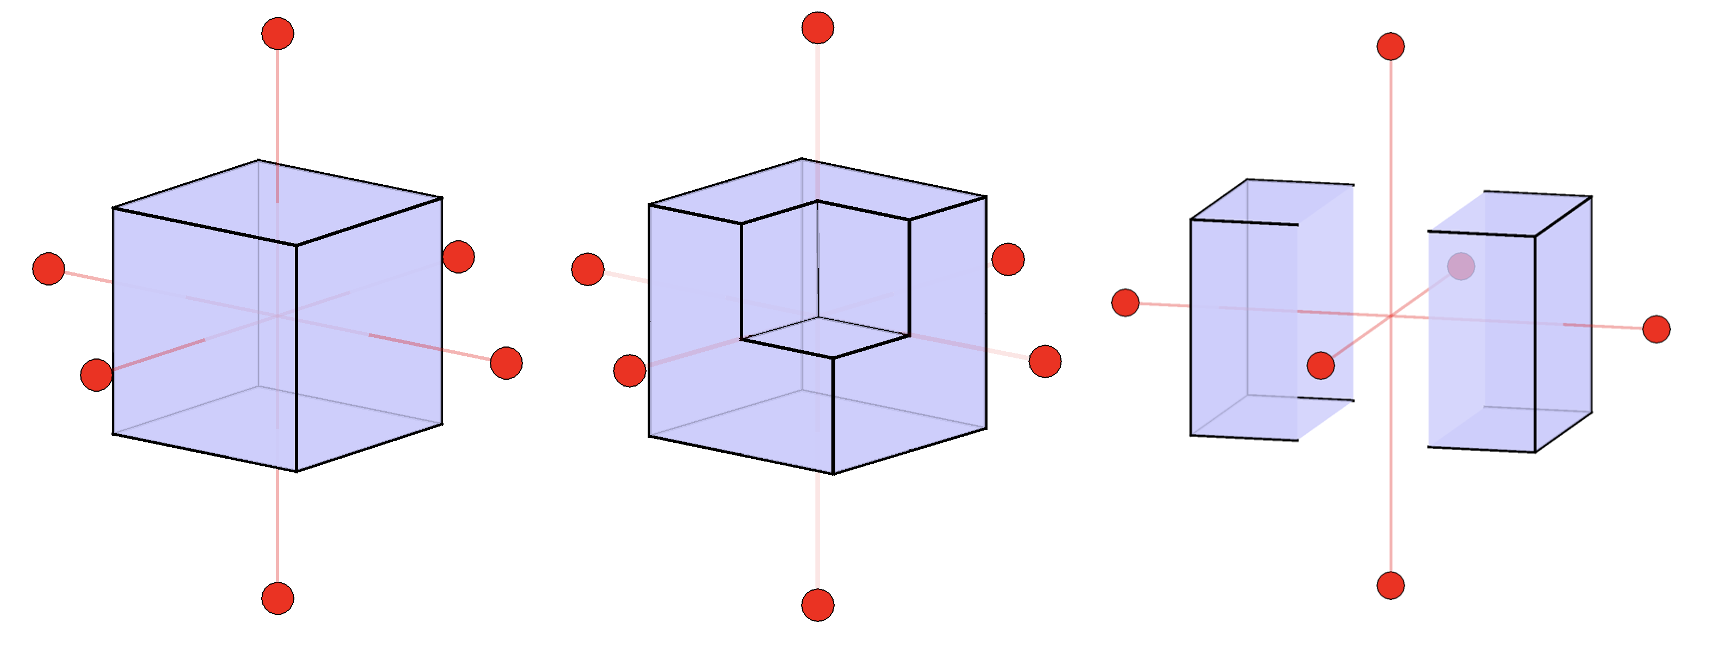
\includegraphics[width=\figmed]{convex_non_open_egis.png}
  \caption{Simplified convex, nonconvex, and open EGI nonuniqueness. Larger circles indicate greater relative areas assigned to a given normal vector.}
  \label{fig:egi_family}
\end{figure}

\subsection{EGI Optimization}

The EGI fulfills two important criteria for the shape inversion problem: it can be estimated directly from the light curve, attitude profile, and material properties, and uniquely represents a convex object \cite{kaasalainen2001}. Further, the EGI can be transformed into a unique convex object and vice versa through the dual transform and Minkowski problem \cite{little1985, minkowski1909}. 

To accomplish the goal of fitting a convex object to a collection of light curve measurements, it is advantageous to define a compact expression for the expected normalized irradiances of a convex object. This is accomplished through the convex reflection matrix $G \in \mathbb{R}^{n \times m}$ with $ij$th entries $G_{ij}$ defined at time $i$ for each facet $j$ is defined using Eq \ref{eq:brdf_def} and Eq \ref{eq:lc_func_normalized} as the normalized received facet irradiance per unit facet area:

\begin{align*} \numberthis \label{eq:reflection_matrix}
  G_{ij} &= \frac{I_{ij}}{I_s a_j} \\
  &= f_r\left(L, O \right) \left(L_j \cdot N_i\right) \left(O_j \cdot N_i\right).
\end{align*}

It must be noted that Eq \ref{eq:reflection_matrix} assumes that the BRDF of the object is uniform across its surface. This is a core assumption of the direct convex inversion scheme in the literature, and a limitation of the method that cannot be easily circumvented. This relationship between the received normalized irradiance and the areas of the object faces reveals the compact form of Eq \ref{eq:lc_func_normalized} for convex objects for any BRDF:

\begin{equation} \label{eq:convex_lc_with_g}
  \check{I}_{convex} = G \vctr{a}.
\end{equation}

Given a light curve, direct shape inversion schemes sample $m$ candidate normal vectors $\vctr{N}$ on the unit sphere to fit an EGI to the observed light curve $\check{I}_\textrm{obs} \in \mathbb{R}^{n \times 1}$ \cite{friedman2020, fan2020thesis}. This is accomplished by solving an optimization problem to distribute the area vector $\vctr{a}$ across the sampled normals to minimize the residual between the observed and modeled light curves. In practice, this is a constrained nonnegative least squares (NNLS) problem and can be solved efficiently for large numbers of normal vectors $\vctr{N}$ and light curve data points $\check{I}_\textrm{obs}$:

\begin{equation} \label{eq:area_opt_convex}
  \min_{\vctr{a}}{\|\check{I}_{\textrm{obs}} - G \vctr{a}\|_2} \:\:\: \textrm{ subject to } \vctr{a}_i \geq 0,
\end{equation}

to yield an optimal set of face areas $\vctr{a}_i$. In Eq \ref{eq:area_opt_convex}, the reflection matrix $G$ is computed from the chosen normal vectors $\vctr{N}_i$, the uniform BRDF, and the Sun and observer vectors in the body frame of the object. NNLS problems are efficiently solved via Lawson and Hanson's original algorithm \cite{lawson1976}, or the more recent Fast NNLS (FNNLS) algorithm due to Bro and De Jong \cite{bro1996}. It is important to note that the area estimated with Eq \ref{eq:area_opt_convex} is the \textit{albedo-area} due to the reflectivity coefficients in Eq \ref{eq:lc_func_normalized} or \ref{eq:lc_normalized_engine}. If the value of $C_d$ and $C_s$ are uniform with a known ratio $C_d / C_s$, the recovered geometry will be scaled without impacting the face adjacency or relative feature sizes.

The optimization in Eq. \ref{eq:area_opt_convex} produces a coarse approximation of the true EGI as $m$ is finite. Increasing $m$ necessarily improves the quality and sparsity of the estimated EGI, but at the cost of computational resources. The estimation was performed using a synthetic light curve input from $n=500$ Sun and observer vectors uniformly sampled on the sphere in the body frame, producing a full rank $G$ matrix. $m = 500$ candidate normal vectors were sampled using a spherical Fibonacci mapping described by Keinert et al.\ in \cite{keinert2015}. Results are visualized for an icosahedron in the body frame in Figure \ref{fig:initial_egi_sampling}. Reconstructing the object at this stage is difficult due to the quantity of faces present in the estimated EGI. 

\graphicspath{{/Users/liamrobinson/Documents/PyLightCurves/docs/build/html/_images}}
\begin{figure}[!htb]
  \centering
  \includegraphics[width=\figmed]{sphx_glr_egi_figs_aas22_002.png}
  \caption{Initial EGI optimization example for a cube, using 500 candidate normal vectors, the Phong BRDF with $C_d=0.5$, $C_s=0.5$, $n=10$. Relative face area denoted by higher sphere opacity, reference shape shown in grey.}
  \label{fig:initial_egi_sampling}
\end{figure}

\subsection{EGI Observability}

For a given set of candidate normal vectors, the ability to recover a reliable solution from the area optimization problem is known as its observability. As studied by Friedman, the EGI optimization is observable if the Gramian matrix --- $G^T G$ in this case --- is full rank \cite{friedman2020}.

This conclusion follows from an unconstrained least squares estimation of the EGI, and is generally equivalent to the statement that the areas of $n$ normal vectors can be estimated if $m>=n$ measurements are taken with at least one nonzero entry in each column of the reflection matrix $G$. As noted by Cabrera et al.\, the nonnegative constraint placed on the face areas $a_j$ mean that the constrained EGI optimization is often estimatable even when the unconstrained form is unobservable \cite{cabrera2021}. As a result, the unconstrained least squares observability condition is a very conservative lower bound, but is still useful for quantifying the shape information content of the light curve through the rank of $G^T G$. All inversions results presented in this work are performed with observable measurement geometry. 

The EGI observability exposes a new shape ambiguity. If any areas of the EGI are unobservable, the geometry of those portions of the object are entirely unconstrained when considering the light curve alone.

\subsection{EGI Resampling}

A normal vector resampling step is presented in this work to promote a more accurate and sparse EGI. The normal vectors used in Fig \ref{fig:initial_egi_sampling} are generally correct, with each group clustering around a normal vector of the truth geometry. This clustering behavior occurs when none of the candidate normal vectors are sufficiently close to the truth. Resampling in a cone centered on each initial EGI normal vector provides more accurate candidates for EGI estimation. This process mimics a single optimization step with a much larger $m$, where the coarse EGI is used to exclude areas on the sphere with little or no normal area.

Uniformly sampling a cone of half-angle $\phi$ is accomplished by strategically sampling points on the unit sphere. 

\begin{equation} \label{eq:cone_sample_n_pole}
  \vctr{N}_{cone} = \begin{bmatrix}
    \sqrt{1-z^2}\cos{\theta} \\
    \sqrt{1-z^2}\sin{\theta} \\
    z \\
  \end{bmatrix}
\end{equation}

In Eq \ref{eq:cone_sample_n_pole} two coordinates are chosen $z \in [\cos{\phi}, 1]$ and $\theta \in [0, 2\pi)$, yielding a point uniformly distributed on a cone of half-angle $\phi$ about the central axis $[0, 0, 1]^T$ \cite{cone_sampling_wolfram}. These points are then rotated using a direction cosine matrix to center the cone on an axis of interest. The axis of rotation for this transformation is the cross product of the original central axis $[0, 0, 1]^T$ with the final axis $\vctr{N}_{cone}$ with the rotation angle $\theta$ being the angle between the same two vectors. The principal rotation parameter form of this transformation is given in Eq \ref{eq:cone_sampling_rv} which can be converted into the DCM using Eq \ref{eq:quat2dcm} and \ref{eq:prp2quat}.

\begin{align*} \label{eq:cone_sampling_rv} \numberthis
  \theta &= 2 \cos^{-1}\left( \vctr{N}_{cone,z} \right) \\
  \lambda &= \vctr{N}_{cone} \times [0, 0, 1]^T
\end{align*}

The number of new candidates sampled per initial solution vector and the cone half-angle should be adjusted on a case-by-case basis depending on the compute power available and light curve data quality. Multiple iterative methods exist for solving nonnegative constrained least squares (NNLS) problems. The classical NNLS algorithm was published by Lawson and Hanson and improved later by Bro and De Jong in their Fast NNLS (FNNLS) approach \cite{lawson1976, bro1996}.

Existing EGI optimization schemes like those of Fan \cite{fan2020thesis}, Friedman \cite{friedman2020}, and Cabrera \cite{cabrera2021} are limited by a single normal vector sampling step, leading to a lack of sparsity in the optimized EGI. High-density normal vector sampling in regions known to contain non-zero area leads to EGI solutions that are generally more sparse and cluster more tightly about true normal vectors. An example of this process is shown in Figure \ref{fig:resampled_egi}.

\begin{figure}[!htb]
  \centering
  \includegraphics[width=\figmed]{sphx_glr_egi_figs_aas22_003.png}
  \caption{Resampled EGI for the cube data using $\phi = \frac{\pi}{20}$, $100$ candidate vectors per resampled cone. Relative face area denoted by higher sphere opacity, reference shape shown in grey.}
  \label{fig:resampled_egi}
\end{figure}

\subsection{EGI Merging}

After resampling and optimizing again with Eq. \ref{eq:area_opt_convex}, the reestimated EGI is merged by computing all groups $\mathcal{G}$ of EGI vectors within an angular offset $\theta_\mathrm{merge}$:

\begin{equation} \label{eq:egi_merge}
  \mathcal{G}_k = \left\{ \vctr{E}_i \in \vctr{E} \:\| \cos^{-1}\left( \frac{\hat{E}_i \cdot \hat{E}_k}{\|\vctr{E}_i \| \| \vctr{E}_k \|}\right) < \theta_\mathrm{merge} \right\}.
\end{equation}

In practice, the choice of $\theta_\mathrm{merge}$ is dependent on the user's tolerance for discretization, as merging will approximate smooth geometry by discrete faces with normal vectors offset by $2\theta_\mathrm{merge}$. Groups are merged by summing all group members, yielding a single EGI vector $\vctr{E}_m$ without loss of closure. 

\begin{equation} \label{eq:fixing_egi}
  \vctr{E}_m = \sum_{\vctr{E} \in \mathcal{G}_k}{\vctr{E}}
\end{equation}

Merging the resampled EGI shown in Figure \ref{fig:resampled_egi} produces a final sparse EGI fit for object reconstruction, shown in Figure \ref{fig:merged_egi}. 

\begin{figure}[!htb]
  \centering
  \includegraphics[width=\figmed]{sphx_glr_egi_figs_aas22_004.png}
  \caption{Merged EGI for the cube data using $\alpha = \frac{\pi}{10}$. Relative face area denoted by higher sphere opacity, reference shape shown in grey.}
  \label{fig:merged_egi}
\end{figure}

\subsection{Geometry Recovery from the EGI}

At this stage, the resampled and merged EGI encodes a convex approximation of the underlying object with no guarantee of the closure of this EGI. The EGI closure constraint Eq \ref{eq:egi_closure} motivates a simple procedure to correct an invalid EGI by adding the mean closure error to each entry:

\begin{equation} \label{eq:egi_validation}
  \vctr{E}_{\textrm{closed}} = \vctr{E}_{\textrm{open}} - \sum_{i=1}^m a_i \vctr{N}_i .
\end{equation}

The concept of a closure step is not a novel contribution. Fan's method solved an optimization problem to adjust the EGI towards closure \cite{fan2020thesis}. This process is improved with a simpler analytical correction. In practice this process should be performed before each reconstruction to accelerate convergence. Failing to correct non-closed EGIs will cause convergence to a nonzero minimum in the reconstruction objective function as there is no corresponding convex object with the given EGI.

The unique convex object encoded by each closed EGI is reconstructed by solving for the polytope's set of vertices $\mathcal{V}$ and faces $\mathcal{F}$ encoding the adjacency relations between vertices. This is accomplished following the procedure introduced by Little through the dual transformation \cite{little1983}. The dual set $\mathcal{D}$ are vertices in $(A, B, C) \in \mathbb{R}^3$ that satisfy the following plane condition for a point $(x, y, z)$ on each face of the object:

\begin{equation} \label{eq:dual_abc_form}
  Ax + By + Cz + 1 = 0
\end{equation}

If $(x, y, z)$ are chosen to be the closest points in the object's planes to the origin, the dual set $\mathcal{D}$ can be expressed in terms of the EGI and a support vector $\vctr{h} \in \mathbb{R}^{\|F\| \times 1}$, where the support vector is the vector of perpendicular distances of each face of the object to the origin. The points of the dual $\mathcal{D}_i \in \mathbb{R}^3$ is expressed in terms of the EGI and the supports as:

\begin{equation} \label{eq:dual_egi_form}
  \mathcal{D}_i = \frac{\vctr{E}_i}{ \| \vctr{E}_i \| \vctr{h}_i}.
\end{equation}

The object's vertices $\vctr{v}_{ref}$ are found by solving a linear system of equations for each face on the convex hull of dual set vertices. Triplets of vertices on the resulting faces are used to find a single real vertex by intersecting the three planes defining the dual set vertices.

\begin{equation} \label{eq:vertex_recovery}
  \begin{bmatrix}
    v_{ref,x} \\
    v_{ref,y} \\
    v_{ref,z} \\
  \end{bmatrix} = \begin{bmatrix}
    v_{i,x} & v_{j,x} & v_{k,x} \\
    v_{i,y} & v_{j,y} & v_{k,y} \\
    v_{i,z} & v_{j,z} & v_{k,z}
  \end{bmatrix}^{-1} \begin{bmatrix}
    1 \\ 1 \\ 1
  \end{bmatrix}
\end{equation}

Convex face adjacency information is found by triangulating the convex hull of all reference vertices. The accuracy of the recovered geometry is entirely dependent on the correctness of the support vector $\vctr{h}$ used to produce the dual set. Finding the true support vector is the challenge of the final optimization in convex shape inversion.

\subsection{Support Vector Optimization}

This work adopts the same objective function proposed by Little for the support vector optimization as used by Fan \cite{little1983, fan2020thesis}. Little's objective function leverages work of Minkowski, who proved that any closed EGI is a unique representation of a convex object, up to a translation \cite{little1983}. In the literature, these convex shapes in $\mathbb{R}^3$ are known as polytopes. In particular, that unique polytope is merely a scaling and translation from the polytope with volume $1$ that minimizes $\vctr{h} \cdot \| \vctr{E} \|$ \cite{little1985}. This formulates the support vector optimization problem:

\begin{align*} \numberthis \label{eq:little_problem}
  & \min_{\vctr{h}}\left\{ \vctr{h} \cdot \| \vctr{E} \| \right\} \\
  & \textrm{such that } \frac{1}{3}\left(\vctr{h} \cdot \vctr{a} \right) = 1
\end{align*} 

Notice that there is a difference between $ \| \vctr{E} \| $, the areas of the faces on the desired polytope, and $\vctr{a}$, the areas of the polytope recovered by constructing a convex object with the dual transform using Eqs \ref{eq:dual_egi_form} and \ref{eq:vertex_recovery}. This means that a convex object must be fully constructed at each step of the optimization to compute the objective function value. This optimization is highly nonlinear, as adjusting the support of one face may dramatically change both the areas of surrounding faces as well as the volume of the resulting polytope. Due to the convexity of the problem, an initial guess of $\vctr{h} = \mathbf{1}$ is sufficient.

Depending on the optimizer, additional function evaluations will be needed to evaluate support gradient as well as the Jacobian of the constraints. Many optimizers struggle with this optimization problem, either due to an inability to meet the constraint or instability that leads to unbounded supports. Little implemented a constrained gradient descent scheme from scratch, showing good results for reconstructing simple objects \cite{little1983}. Gardner solved an equivalent optimization problem using an unspecified solver in MATLAB \cite{gardner2003}. In this work, trust-region methods \cite{conn2000} were found to be robust at solving this optimization.

\section{Direct Nonconvex Shape Inversion}

\subsection{Nonconvex Feature Detection and Location}

Many human-made space objects are, as highlighted in Figure \ref{fig:hst_bennu_shadows}, highly nonconvex. As a result, their shape inversion is plagued by the fact that the Minkowski problem-driven reconstruction methods of Eq \ref{eq:little_problem} cannot recover nonconvex features. Instead of beginning from the ground up, the convex shape guess can be leveraged to detect and locate concavities.

Information about large, unilateral object concavities is obtained during EGI estimation in Eq. \ref{eq:area_opt_convex} by relaxing the EGI closure constraint. This unconstrained form is also generally functional for most convex objects and can be used without loss of detail in the final reconstruction as long as closure correction in Eq. \ref{eq:fixing_egi} is still employed.

The mean axis of prominent concave features is determined by measuring the divergence of the optimized EGI from a closed object with the magnitude of the closure error $\vctr{e}_{EGI}$.

\begin{equation} \label{eq:closure_error}
  \vctr{e}_{EGI} = -\sum_{i=1}^{m} a_i \vctr{N}_i.
\end{equation}

The EGI closure error vector in Eq \ref{eq:closure_error} represents the missing area on each body axis that could be added to close the object. The addition of the minus sign transforms the vector from expressing the presence of excess area to the absence of missing area. The closure error will be negligible if there are no concavities present. The closure error may also be negligible if there is no self-shadowing present over the sampled attitude profile, therefore the closure error merely quantifies the self-shadowing present in the measurements, not whether there may be self-shadowing in other orientations.

Under the strong assumption that the concavities present are major and unilateral, this EGI error vector points along the mean axis of the concavity. This is because self-shadowing in that region causes brightness measurements to be smaller than expected for the true area present, leading to an optimized EGI that attributes less area to that section of the object. As a result, summing the EGI entries produces a vector that points away from the concavity, requiring the negation seen in Eq \ref{eq:closure_error} to point towards it.

\subsection{Concavity Creation}

Given the direction of a supposed concavity in the body frame of the object, the next challenge is introducing that concavity. This work approximates unknown concave features as valleys with sharp floors, adopting the interior angle $\psi$ between the valley walls as the measure of the feature depth. An interior angle of $\psi=180^\circ$ implies no concavity, whereas $\psi \rightarrow 0^\circ$ will push the concavity through the object entirely.

The proposed process for creating an accurate concavity in the reconstructed convex guess proceeds in four major steps. The model is first subdivided to add more faces and vertices. Subdivided vertices are then classified by their proximity to the EGI error vector, indicating whether their positions should be updated. Boundary vertices are identified, and vertex positions are updated based on an internal angle. The light curve error of that nonconvex guess is computed, and the internal angle is iterated until a suitable minimum error case is identified.

\subsection{Model Subdivision}

Subdividing the initial convex object guess is essential for retaining object detail during concavity creation. A combination of linear subdivision, Loop subdivision, and remeshing algorithms are used to accomplish this. Linear subdivision is advantageous when object faces are equally sized and boundary edges must be maintained. Loop subdivision is preferable when there are numerous vertices so that subdivisions do not drastically diverge from the initial boundary surface. Loop subdivision softens sharp edges as it relies on B-splines to interpolate new vertex positions \cite{loop1987}. The specific type and resolution of subdivision used depends on the level of detail the user needs to maintain in the introduced concavity, although linear subdivision followed by Loop subdivision is a useful baseline. Varying combinations of subdivision are shown in Figure \ref{fig:subd_grid} to illustrate the available configurations.

\graphicspath{{/Users/liamrobinson/Documents/msthesis/static_images/aas_2022_figs}}
\begin{figure}[!htb]
  \centering
  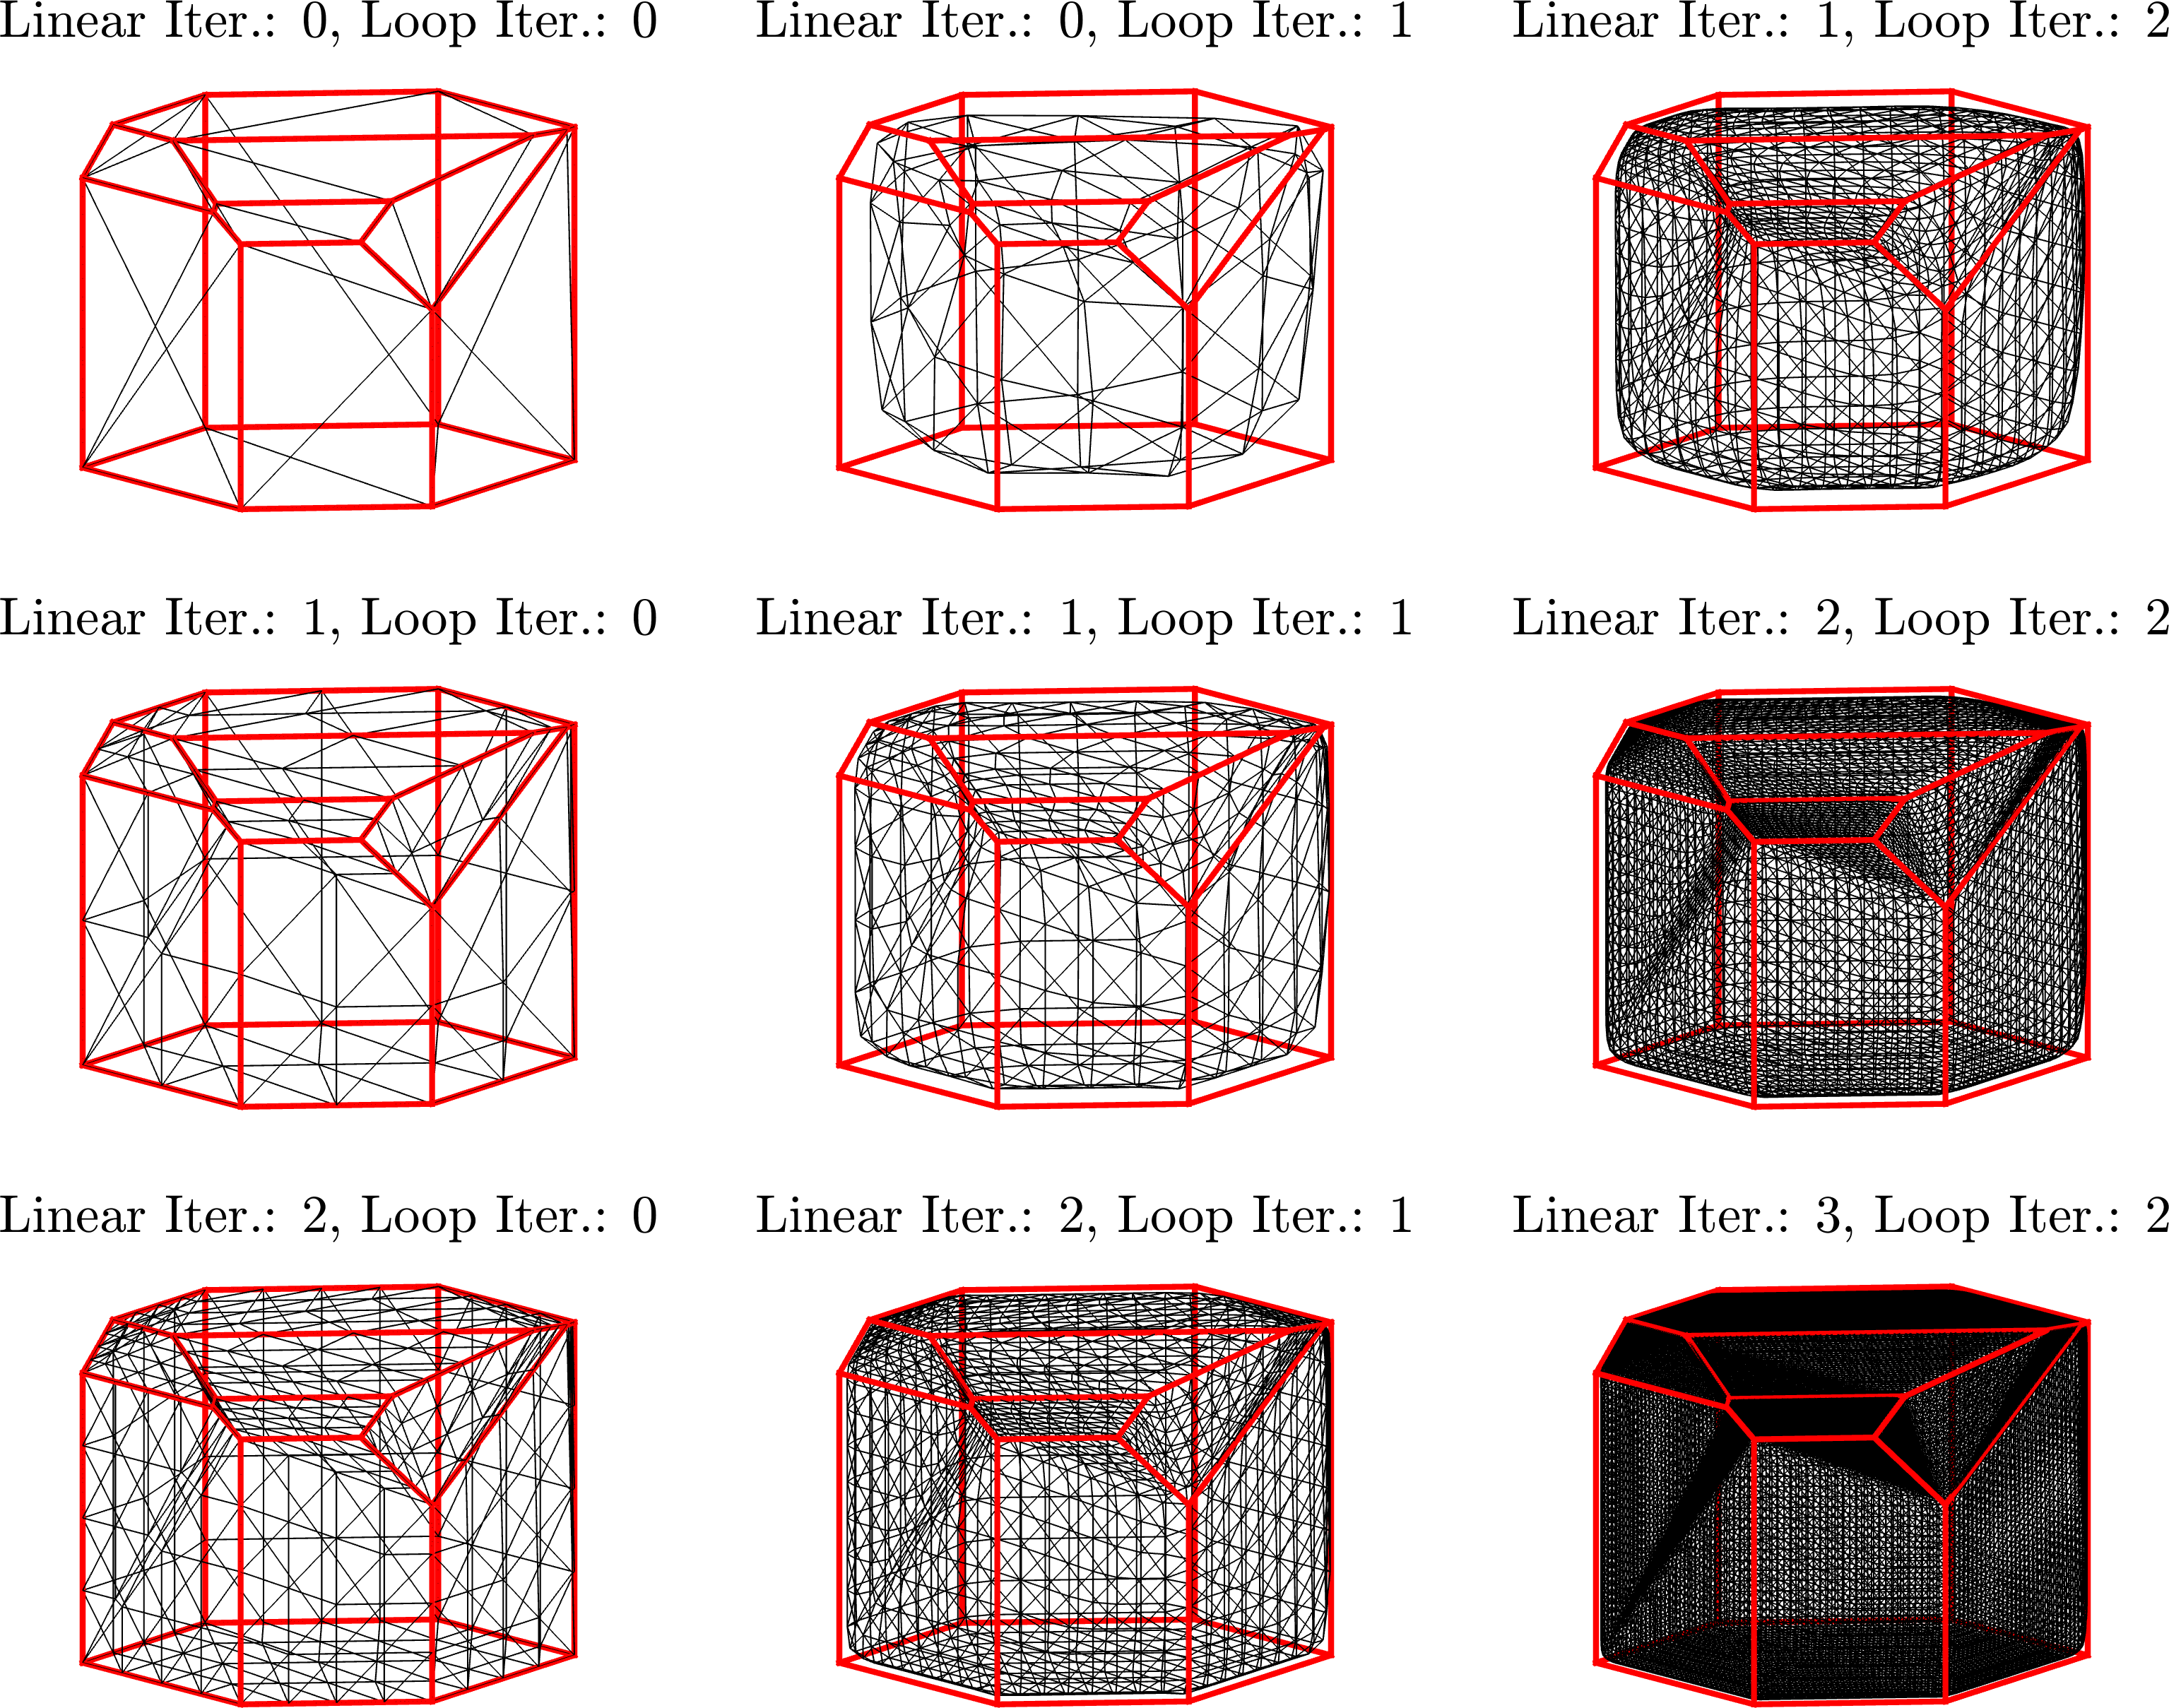
\includegraphics[width=350px]{subd_grid.png}
  \caption{Subdivided object (black) with reference (red) with various levels of subdivision}
  \label{fig:subd_grid}
\end{figure}

\subsection{Vertex Classification}

When introducing a concavity, it is important to classify which vertices are part of the concave feature --- and therefore need to be updated --- and which vertices should remain unaffected. This is accomplished by measuring the angle from each face normal to the EGI error vector, where faces with normal vectors within an angle of $\pi/2 - \varepsilon$ to the error vector must be updated, where $\varepsilon$ is a bias angle that controls the conservativeness of the classification. Choosing $\varepsilon=0$ selects all faces above the horizon from the EGI error vector and may lead to concavities that encompass too much of the object. Generally, $\varepsilon \in [0.3, 0.7]$ rad is effective. In reality, all face normals and areas are impacted by the presence of the concavity in the area optimization Eq. \ref{eq:area_opt_convex} and EGI correction step Eq \ref{eq:egi_validation}. This bound tends to produce visually accurate concavities. Faces requiring an update are termed \textit{free} faces, with all others termed \textit{root} faces. Explicitly, each face $F_i$ is classified $C(F_i)$ via:

\begin{equation} \label{eq:root_free}
  C(F_i) = \begin{cases} 
    0 & \cos^{-1}\left( \vctr{N}_i \cdot \hat{e}_{EGI} \right) \geq \frac{\pi}{2} - \varepsilon \\
    1 & \cos^{-1}\left( \vctr{N}_i \cdot \hat{e}_{EGI} \right) < \frac{\pi}{2} - \varepsilon \\
  \end{cases}.
\end{equation}

In Eq \ref{eq:root_free}, $C(F_i) = 0$ implies a root face, with $C(F_i) = 1$ implying a free face. Vertices on free faces are further classified as being \textit{root-adjacent} or \textit{free}. Root-adjacent vertices are part of at least one root face, whereas free vertices belong to only free faces. The classification of each vertex $\vctr{v}_i$ via $C(\vctr{v}_i)$ is expressed via:

\begin{equation} \label{eq:root_free_verts}
  C(\vctr{v}_i) = \begin{cases}
    0 & \sum_{j \in \mathcal{N}(\vctr{v}_i)}{C(F_j)} = 0 \\
    1 & \sum_{j \in \mathcal{N}(\vctr{v}_i)}{C(F_j)} > 0 \\    
  \end{cases} \: \: \forall i \in \left\{ i \mid C(F_i) = 1 \right\}.
\end{equation}

In Eq \ref{eq:root_free_verts}, $\mathcal{N}(\vctr{v}_i)$ is the set of face indices including $\vctr{v}_i$ as a vertex, yielding $C(\vctr{v}_i) = 0$ to imply a free vertex, and $C(\vctr{v}_i) = 1$ to imply a root-adjacent face. Classifying vertices in this way results in a border of root-adjacent vertices around the interior free vertices, visualized in Figure \ref{fig:root_and_free}.

\begin{figure}[!htb]
  \centering
  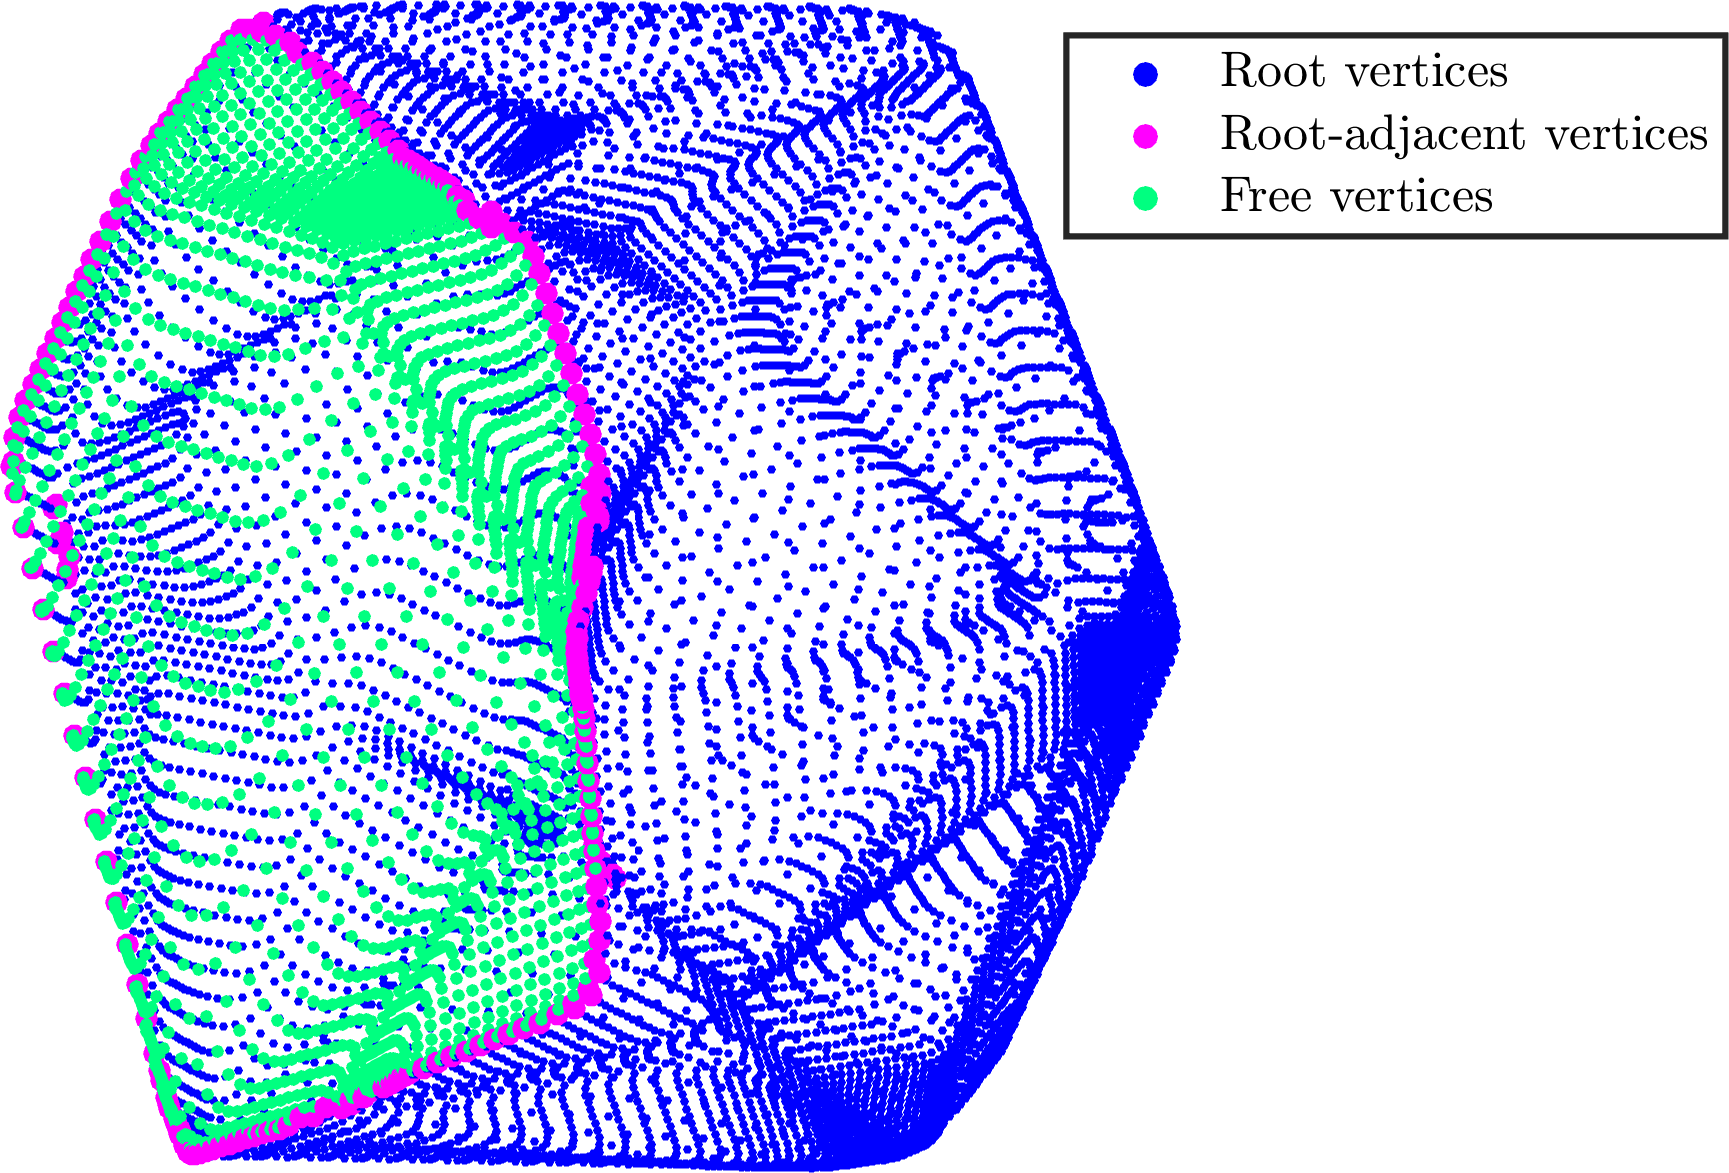
\includegraphics[width=250px]{rootadj_and_free_verts_try2.png}
  \caption{Root-adjacent and free vertices}
  \label{fig:root_and_free}
\end{figure}

\subsection{Vertex Displacement}

Given the estimated internal angle $\psi_{est}$ and the error vector $\hat{e}_{EGI}$, each $i$th free vertex is displaced to introduce a geometrically accurate concavity by moving each a distance $d_i$ in the direction of $-\hat{e}_{EGI}$:

\begin{equation} \label{eq:flip_depth}
  d_i = p_i \sqrt{\csc^2 \frac{\psi_{est}}{2} - 1},
\end{equation}

where $p_i$ is the distance from each $i$th free vertex to the nearest root-adjacent vertex.

\subsection{Internal Angle Iteration}

Prior work by the author indicated an analytical relationship between this interior angle and the norm of the EGI error vector, summarized in Figure \ref{fig:misleading_egi_error} \cite{robinson2022}.

\begin{figure}[!htb]
  \centering
  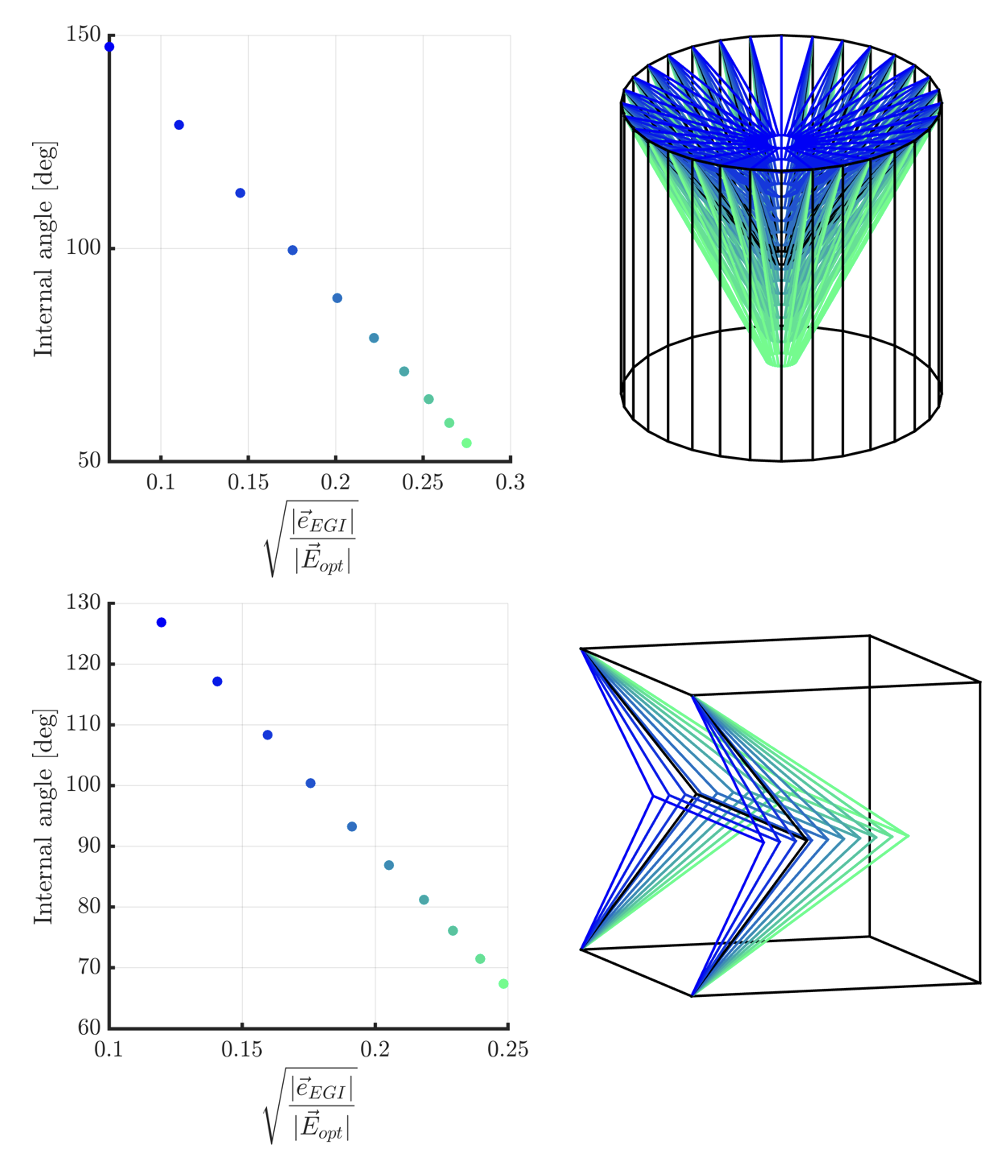
\includegraphics[width=\figsmall]{error_mag_study/combined_error_mag.png}
  \caption{EGI error relationship to internal angle for the collapsed cylinder and collapsed house from \cite{robinson2022}}
  \label{fig:misleading_egi_error}
\end{figure}

The objects in Figure \ref{fig:misleading_egi_error} were illuminated with a simple Lambertian BRDF and the brightness measurements used to optimize the EGI were produced by randomly sampled Sun and observer vectors. Once specular effects and non-random observation conditions are accounted for, the linear relationship between $\psi$ and $\sqrt{\frac{\|\vctr{e}_{EGI}\|}{\|\vctr{E}\|}}$ no longer exists. In short, the optimal concavity angle $\psi_{opt}$ is sought such that:

\begin{equation} \label{eq:psi_opt}
  \psi_{opt} = \min_{\psi} \left( \| \check{I} - \check{I}(\psi) \| \right),
\end{equation}

where $\check{I}$ is the observed normalized light curve and $\check{I}(\psi)$ is the light curve resulting with Eq \ref{eq:lc_normalized_engine} using a nonconvex mesh with a concavity of angle $\psi$ introduced. In practice, a line search is sufficient to find the interior angle that minimizes the light curve error of the reconstructed object, summarized in Algorithm \ref{alg:concavity_iter}.

\begin{algorithm}
  \caption{Concavity sizing algorithm}\label{alg:concavity_iter}
  \begin{algorithmic}
    \State $f_{cvx},v_{cvx}$ \Comment{Faces and vertices of the convex guess}
    \State $f_{subd}, \:v_{subd} \gets \mathrm{Subdivide}(f_{cvx},v_{cvx})$ \Comment{Subdivided convex guess}
    \State $\psi = 180^\circ$ \Comment{Initial guess, no concavity}
    \State $i = 0$ \Comment{Iteration number}
    \While {$i < i_{max}$}
      \State $f_{disp}, \:v_{disp} = \mathrm{DisplaceVertices}(f_{subd},v_{subd})$
      \State $\check{I}_{i} = \mathrm{LightCurve}(f_{disp}, \:v_{disp})$
      \State $e_i = \| \check{I} - \check{I}_{i} \|$
      \State{$\psi \gets \psi + \Delta \psi$}
      \State{$i \gets i + 1$}
    \EndWhile

    $\psi_{opt} = \min_i{e_i}$
  \end{algorithmic}
\end{algorithm}

\section{Shape Inversion With Noisy Measurements}

When the light curve measurements are subject to environmental noise, the shape inversion result --- convex or nonconvex --- may vary significantly from the noiseless shape estimate. Fan addressed this problem most recently with a multiple hypothesis scheme \cite{fan2020thesis}. Given a number of noisy light curves, Fan produced a convex shape estimate from each and ranked each by its error when simulated against a new set of observations \cite{fan2020thesis}. Fan and Frueh later adapted this scheme with a sequential Monte Carlo method, which began identically by producing a collection of convex guesses from samples of the same noisy light curve \cite{fan20201}. The error in each guess was measured against a new noisy light curve, enabling a weighted merge of the estimated EGIs, which was then perturbed to produce a new set of estimated shapes \cite{fan2021}. Throughout these methods, Fan assumed that the noise on the light curve was Gaussian and of constant magnitude, although it was noted that the real character of the noise is dependent on both the geometry of the observation and the magnitude of the signal itself \cite{fan2020thesis}. 

This work presents a method for multiple hypothesis shape inversion that builds on Fan's work by relaxing the constant, Gaussian noise assumption and is agnostic to the convexity of the candidate objects. This new method also uses an face-dependent estimate of the uncertainty in each candidate shape's geometry, yielding final object estimates that take only the most accurate features from each candidate object.

\subsection{Weighted Shape Interpolation}

To develop this multiple hypothesis inversion procedure that works for both convex and nonconvex shape candidates, it is useful to be able to take a weighted average of an arbitrary set of triangle meshes. Given candidate object meshes $M_i$ with scalars $w_i$, this weighted average process should be of the form:

\begin{equation}
  M_{\mathrm{interp}} = \sum_{i}{w_i M_i}.
\end{equation}

The algorithm presented in this work for weighted mesh averaging depends on signed distance fields (SDFs). The SDF implicitly represents a shape by associating each point $\vctr{x} \in \mathbb{R}^3$ with the distance to the closest point on the surface of the object \cite{baerentzen2002}. As a result, the gradient of the SDF points directly away from the closest piece of the object's geometry. For a given SDF $f(\vctr{x})$, the surface of the object $\mathcal{S}_\mathrm{obj}$ is given by all points $\vctr{x}$ that yield $f(\vctr{x}) = 0$:

\begin{equation} \label{eq:sdf_zero_level_set}
  \mathcal{S}_\mathrm{obj} = \left\{ \vctr{x} \in \mathbb{R}^3 \mid f(\vctr{x}) = 0 \right\}.
\end{equation}

Computing the SDF of a triangulated mesh breaks down into computing distances from the points, line segments, and planes making up the mesh to the queried point \cite{baerentzen2002}. A slice of the SDF of a test model is displayed in Figure \ref{fig:sdf_slice}.

\graphicspath{{/Users/liamrobinson/Documents/PyLightCurves/docs/build/html/_images}}
\begin{figure}[!htb]
  \centering
  \includegraphics[width=\figmed]{sphx_glr_sfds_001_2_00x.png}
  \caption{SDF slice of the Stanford bunny model}
  \label{fig:sdf_slice}
\end{figure}

Interpolating three-dimensional meshes using signed distance fields is not a novel concept proposed by this work. Cohen-Or et al.\ used distance fields with anchor points to find warping functions between two geometries \cite{cohen_or1998}. A simple interpolation strategy between two shapes can be accomplished through a weighted average of the respective SDFs. If both objects are weighted at $50\%$, the weighted sum of their SDFs produces a surface that lies halfway in between the two original shapes, measured perpendicular to the input objects' surfaces. This interpolated zero level set surface can be extracted through any three-dimensional isocontouring algorithm such as marching cubes \cite{lorensen1987} or flying edges \cite{schroeder2015}. For example, interpolating between a torus and an icosahedron using this method yields Figure \ref{fig:interpolating_torus_ico}. 

\begin{figure}[!htb]
  \centering
  \includegraphics[width=\figmed]{sphx_glr_shape_interpolation_001.png}
  \caption{SDF interpolation between a torus and an icosahedron}
  \label{fig:interpolating_torus_ico}
\end{figure}

The proposed algorithm for shape interpolation for SDF interpolation of two shapes $M_1, M_2$ with convex weights $w_1, w_2$ is:

\begin{algorithm}
  \caption{SDF interpolation}\label{alg:sdf_interp}
  \begin{algorithmic}
  \Require $w_1 + w_2 = 1$
  \State $\mathrm{SDF}_{\textrm{interp}} \gets w_1 \cdot \mathrm{SDF}_{M_1} + w_2 \cdot \mathrm{SDF}_{M_2}$
  \State $M_{\textrm{interp}} = \mathrm{Isocontour}(\mathrm{SDF}_{\textrm{interp}}, 0)$.
  \end{algorithmic}
\end{algorithm}

Algorithm \ref{alg:sdf_interp} can operate on arbitrary convex or nonconvex meshes, making it well suited to interpolating between light curve inversion results.

The procedure in Algorithm \ref{alg:sdf_interp} can be further generalized by allowing the weights $w_i$ to be functions of the location in $\mathbb{R}^3$ of each SDF grid point:

\begin{equation}
  \mathrm{SDF}_{\mathrm{interp}}(x, y, z) = w_1(x, y, z) \cdot \mathrm{SDF}_{M_1}(x, y, z) + w_2 \cdot \mathrm{SDF}_{M_2}(x, y, z).
\end{equation}

To discourage degenerate behavior, it is necessary to enforce $w_i(x,y,z) > 0 \forall (x,y,z) \in \mathbb{R}^3$.

\subsection{Shape Estimate Uncertainty}

When merging multiple inaccurate shape guesses it is advantageous to measure the uncertainty in each candidate shape and use that uncertainty as a weighting to bias the merging process. The formulation used in this work relies on two face-wise uncertainty terms. First, a face should have high uncertainty if very little light would have reflected off that face to contribute to the light curve. Second, that face should also have high uncertainty if its reflected light has highly contaminated by background noise. As a result, the only faces of an estimated shape with low uncertainty should be those that reflect a large \textit{quantity} of light, increasing the observability of that face, while being uncontaminated by the background to yield a high \textit{quality} signal. These uncertainty terms are computed by first scaling the columns of the reflection matrix defined in Eq \ref{eq:reflection_matrix} by the area of each respective face $a_j$:

\begin{equation} \label{eq:h_matrix}
  H_{ij} = a_j G_{ij}.
\end{equation}

The resulting matrix $H$ has the same dimensions as $G$, but has entries $H_{ij}$ representing the normalized irradiance expected from face $j$ and time $i$. The total normalized irradiance over all timesteps for each face is given by:

\begin{equation} \label{eq:total_norm_irrad}
  \check{I}_{j} = \sum_{i}{H_{ij}}.
\end{equation}

Computing $\check{I}_{j}$ is useful as it represents the total quantity of signal expected from face $j$ across the light curve. Using this value, the data quantity weighting is:

\begin{equation} \label{eq:unc_quantity}
  u_{quant,j} = 1 - \frac{\check{I}_{j} - \min_{j}{\check{I}_{j}}}{\max_{j}{\check{I}_{j}} - \min_{j}{\check{I}_{j}}}.
\end{equation}

Interpreting Eq \ref{eq:unc_quantity}, the face with the most influence on the overall light curve is assigned a data quantity uncertainty of $u_{quant,j} = 0$ while the face with the least influence is assigned $u_{quant,j} = 1$. This meets the first requirement for the uncertainty measure sought; a large quantity of data should produce an accurate final shape estimate. This is further motivated by investigating the statistical nature of the light curve signal. As the object signal is Poisson distributed, the signal itself is well-modeled as a Poisson distribution independently sampled at each timestep. Since the sum of two Poisson distributions with mean and variance $\lambda_1$ and $\lambda_2$ is also Poisson with parameter $\lambda_3 = \lambda_1 + \lambda_2$, the total variance of the sum of the light curve $\lambda_\mathrm{lc}$ is:

\begin{equation}
  \lambda_\mathrm{lc} = \sum_{i} C_{obj,meas,i},
\end{equation}

implying that as the sum of the signal magnitudes grow linearly, their standard deviation $\sqrt{\lambda_\mathrm{lc}}$ grows sublinearly. As a result, a higher quantity of available data for a face will will always exponentially lower the SNR. That said, a high quantity of available data does not necessarily mean that the data has a high SNR. Estimating the SNR in the measured counts is certainly possible, especially if the observing station is well characterized, but is a strong assumption for an unknown ground station. It would be preferable to estimate the variance of the measured signal through the convex shape guess itself. As the NNLS optimization of the EGI is guaranteed to produce the convex shape that best matches the measured irradiances, the convex guess is a good estimator for the mean of the received signal so long as the noise on the measurements is zero mean. As a result, the variance of the light curve error:

\begin{equation}
  \mathrm{Var}\left(\delta \check{I}\right) = \mathrm{Var}\left(Ga - \check{I}_{meas}\right)
\end{equation}

generally matches the true signal and noise variance. This means that scaling the expected normalized irradiance $H_{ij}$ by the absolute value of the light curve error yields a quantity that is proportional to the number of false counts above or below the true mean attributed to a certain face:

\begin{equation}
  \delta \check{I}_{tot,j} = a_j \sum_{i}{\left( G_{ij} a_j - \check{I}_{meas,i} \right) H_{ij}},
\end{equation}

yielding a weighting for the data quality attributed to each face of the convex guess:

\begin{equation} \label{eq:u_qual}
  u_{qual,j} = \frac{\delta \check{I}_{tot,j} - \min_{j}{\delta \check{I}_{tot,j}}}{\max_{j}{\delta \check{I}_{tot,j}} - \min_{j}{\delta \check{I}_{tot,j}}}.
\end{equation}

Eq \ref{eq:u_qual} can be interpreted in terms of the statistical properties of the light curve just like Eq \ref{eq:unc_quantity}. Under the assumption that the EGI optimized by NNLS produces a good estimator for the mean of the measured light curve, higher environmental noise will produce a larger residual $\delta \check{I}_{tot,j}$ at a given signal magnitude. As a result, the term $u_{quant,j}$ can be seen as accounting for the variance of the object signal --- which becomes less impactful as the object signal grows --- while the term $u_{qual,j}$ acocunts for the variance of the environmental noise --- which acts to degrade the light curve signal regardless of the object signal magnitude.

These two uncertainty weightings are combined at each face for a global uncertainty estimate:

\begin{equation} \label{eq:u_total}
  u_{j} = \frac{u_{qual,j}}{2} + \frac{u_{quant,j}}{2}.
\end{equation}

Eq \ref{eq:u_total} is formulated such that a face is only assigned a low uncertainty if it has both high data quality and quality. A face with the lowest quality and quantity will be assigned $u_{j} = 1$ while simply having bad quality or quantity alone yields $u_j = 0.5$, thereby discounting low quantities of high quality data as well high quantities of low quality data. Figure \ref{fig:face_uncertainties} displays the quality, quantity, and overall uncertainty weighting for the faces of a convex shape guess.

\begin{figure}
  \centering
  \begin{subfigure}[b]{0.3\textwidth}
      \centering
      \includegraphics[width=\textwidth]{sphx_glr_face_uncertainty_005.png}
      \label{fig:quant_weights}
  \end{subfigure}
  \hfill
  \begin{subfigure}[b]{0.3\textwidth}
      \centering
      \includegraphics[width=\textwidth]{sphx_glr_face_uncertainty_006.png}
      \label{fig:qual_weights}
  \end{subfigure}
  \hfill
  \begin{subfigure}[b]{0.3\textwidth}
      \centering
      \includegraphics[width=\textwidth]{sphx_glr_face_uncertainty_007.png}
      \label{fig:qual_overall}
  \end{subfigure}
  \caption{Quantity (left), quality (middle), and overall face uncertainty (right) weights}
  \label{fig:face_uncertainties}
\end{figure}

Figure \ref{fig:face_uncertainties} conveys that $u_{qual}$ and $u_{quant}$ convey independent information about each face depending on the measured light curve and its noise --- higher data quantity does not necessarily imply higher quality.

\subsection{Spherical Nearest Neighbor Weights} \label{sec:nearest_sphere}

One final challenge remains: translating the uncertainties of the faces of an object to a weighting function that can be applied throughout $\mathbb{R}^3$ to weight the SDF. Simply projecting points onto the unit sphere and performing nearest-neighbor interpolation accomplishes this task well. For a set of reference points $\vctr{r}_{i}$ each with a weight $w_i$, the weight index $i_q$ of query point $\vctr{r}_q \in \mathbb{R}^3$ is the solution to:

\begin{equation}
  i_{q} = \min_{i}\left( \| \vctr{r}_q - \vctr{r}_i \| \right).
\end{equation}

In practice, this is solved with a Balltree, a spatial search data structure designed to efficiently find nearest neighbors in $n$-dimensional space bounded by the $n-1$-dimensional sphere \cite{omohundro1989}. The result of this nearest neighbor interpolation for a number of query points is shown in Figure \ref{fig:ball_tree_nn_interp}.

\begin{figure}[!htb]
  \centering
  \includegraphics[width=\figmed]{sphx_glr_spherical_voronoi_interp_001.png}
  \caption{Nearest neighbor interpolation between reference points (red) with uniformly distributed weights on $[0,1]$.}
  \label{fig:ball_tree_nn_interp}
\end{figure}

The final spherical weighting $w(\vctr{r}_q)$ applied to each object at a given query point location $\vctr{r}_q \in \mathbb{R}^3$ is the certainty of the nearest face $1-u_j(\vctr{r}_q)$ scaled by the light curve error of that object:

\begin{equation} \label{eq:merge_weighting}
  w(\vctr{r}_q) = \left( 1-u_j(\vctr{r}_q) \right) \left( \check{I}_{meas} - \check{I}_\mathrm{obj} \right),
\end{equation}

where $\check{I}_{meas}$ is the measured normalized light curve produced by Eq \ref{eq:ihat_meas} and $\check{I}_\mathrm{obj}$ is the normalized light curve produced by the shape estimate under the same observation conditions.

\subsection{Full Noisy Inversion Procedure} \label{sec:mh_inversion}

Given $n$ noisy light curves from an object of unknown shape, the procedure determining a single best estimate of the object's true shape has three stages. 

\begin{enumerate}
  \item Convex shape guesses are computed for each noisy light curve.
  \item Each shape is checked for potential nonconvex features by introducing singular concavities in the direction of the EGI error vector following Algorithm \ref{alg:concavity_iter}. Each nonconvex guess along with the convex guess is simulated in the same observation conditions to compute an error with respect to the original light curve. The guess --- convex or nonconvex --- with the lowest error is selected moving forward.
  \item Now with $n$ convex or nonconvex shape estimates, one for each original light curve, the uncertainty in each face of each object is computed with Eq \ref{eq:u_total}.
  \item Given these uncertainties, each object is assigned a spherical weighting function $w_i(x, y, z)$ via Eq \ref{eq:merge_weighting}.
  \item The objects are merged together via their weights using the SDF procedure outlined by Algorithm \ref{alg:sdf_interp}, yielding a final shape estimate.
\end{enumerate}



%%% RESULTS

%%% CONCLUSION
\ProvidesFile{ch-recommendations.tex}[2022-10-05 recommedations chapter]

\chapter{RECOMMENDATIONS}

Buy low.
Sell high.

\ProvidesFile{ch-appendices.tex}[Appendices]
\chapter{Appendices}

\section{Shadow Mapping} \label{data:shadow_mapping}

\subsection{Shading} \label{data:shading}

\begin{algorithm}
  \caption{Pixel-wise shading algorithm with shadow mapping}\label{alg:pix_shading}
  \begin{algorithmic}
    \State $L \in \mathbb{S}^2$ \Comment{Unit vector from object origin towards Sun}
    \State $O \in \mathbb{S}^2$ \Comment{Unit vector from object origin towards observer}
    \State $N \in \mathbb{S}^2$ \Comment{Outward-pointing surface normal vector at pixel coordinates}
    \State $(C_d, C_s, n) \in \mathbb{S}^2$ \Comment{Reflection coefficients and exponent for the BRDF}
    \Require $C_d + C_s \leq 1$ \Comment{Enforce energy conservation}
    \State $MVP_{Sun} \in \mathbb{R}^{4 \times 4}$ \Comment{MVP matrix for the Sun camera}
    \State $(x, y) \in \mathbb{Z}^2$ \Comment{Integer pixel coordinates from the observer camera}
    \State $R_{pix,obs} \in \mathbb{R}^3$ \Comment{World coordinates of the pixel; provided by OpenGL}
    \State $\left[(x_{homo,Sun}, y_{homo,Sun}, ...\right] \gets MVP_{Sun} \left[ R_{pix,obs}, 1 \right]^T$
    \State $x_{Sun} \gets \left(1 + p_{x, homo}\right) \frac{w_\mathrm{pix}}{2} $ \Comment{Homogeneous coordinates from the Sun camera}
    \State $y_{Sun} \gets \left(1 + p_{y, homo}\right) \frac{a \cdot w_\mathrm{pix}}{2} $
    \State $D_{Sun} \gets  d(x_{sun}, y_{sun})$ \Comment{Closest pixel depth to the Sun direction}
    \State $D_\mathrm{obs} \gets \left( L - O \right) \cdot L$ \Comment{Closest pixel depth in the Observer direction}
    \If{$D_\mathrm{obs} > D_{Sun}$}
      \State $\delta_{ss} = 1$ \Comment{Pixel is self-shadowed}
    \Else 
      \State $\delta_{ss} = 0$ \Comment{Pixel may be illuminated}
    \EndIf
    \If{$\left(N \cdot L\right) > 0 \textrm{ and } \left(N \cdot O\right) > 0$}
      \State $f_r(\vctr{x}, L, O) = 0$ \Comment{Pixel cannot be both observed and illuminated}
    \Else 
      \State $f_r(\vctr{x}, L, O) = \mathrm{Phong}(L, O, N, C_d, C_s, n)$ \Comment{The pixel is shaded with the BRDF}
    \EndIf
    \State $\mathrm{IM}(x, y) = f_r(\vctr{x}, L, O) \left(N \cdot L\right) $ \Comment{Image pixel value}
  \end{algorithmic}
\end{algorithm}

\clearpage
\section{Astronomical Spectra Data} \label{data:spectra}

\subsubsection{Atmospheric Extinction} \label{data:atm} Data from \cite{krag2003}.
The atmospheric extinction coefficient is dimensionless.
\begin{listing}[H]
\inputminted[breaklines=true, breakanywhere=true, breaksymbol=\hspace{0pt}, fontsize=\footnotesize]{json}{/Users/liamrobinson/Documents/PyLightCurves/mirage/resources/data/atmos_extinction.json}
\end{listing}

% \subsubsection{Quantum Efficiency} \label{data:qe}
% The quantum efficiency spectrum has units $\left[ \frac{e^-}{m} \right]$.
% \begin{listing}[H]
% \inputminted[breaklines=true, breakanywhere=true, breaksymbol=\hspace{0pt}, fontsize=\footnotesize]{json}{/Users/liamrobinson/Documents/PyLightCurves/mirage/resources/data/kaf16803_quantum_efficiency.dat}
% \end{listing}

\subsection{Lunar Phase Factor}
The lunar phase factor is a function of the phase angle in radians and is dimensionless. Data from \cite{daniels1977}.
\begin{listing}[H]
\inputminted[breaklines=true, breakanywhere=true, breaksymbol=\hspace{0pt}, fontsize=\footnotesize]{json}{/Users/liamrobinson/Documents/PyLightCurves/mirage/resources/data/lunar_phase.json}
\end{listing}

\clearpage
\subsection{Scattered Moonlight}
The scattered moonlight radiance in $\left[ \frac{W}{sr \cdot m^2 \cdot m} \right]$ is a function of the difference in the line of sight and Moon azimuths \texttt{delta\_az} in radians, the zenith angle of the Moon \texttt{z\_moon} in radians, and the zenith angle of the line of sight \texttt{z\_obs} in radians. Data from \cite{daniels1977}.

\begin{listing}[H]
\inputminted[breaklines=true, breakanywhere=true, breaksymbol=\hspace{0pt}, fontsize=\footnotesize]{json}{/Users/liamrobinson/Documents/PyLightCurves/mirage/resources/data/moonlight.json}
\end{listing}

\clearpage
\subsection{Zodiacal Light} \label{data:roach_zod}

The zodiacal light surface brightness in $S_10$ is a function of the latitude \texttt{"ecliptic\_lat"} and longitude \texttt{"ecliptic\_lon"} of the line of sight in the solar system ecliptic reference frame, both expressed in radians. Data from \cite{roach1972}.

\begin{listing}[H]
\inputminted[breaklines=true, breakanywhere=true, breaksymbol=\hspace{0pt}, fontsize=\footnotesize]{json}{/Users/liamrobinson/Documents/PyLightCurves/mirage/resources/data/zodiacal.json}
\end{listing}

\clearpage
\section{Telescope Parameters}

\subsubsection{Purdue Optical Ground Station}

\begin{table}[ht]
    \centering
    \begin{tabular}{|l|l|}
    \hline
    \textbf{Parameter} & \textbf{Value} \\ \hline
    FWHM                & $1.5$                              \\ \hline
    Sensor dimensions    & $ 0.03690 \times 0.03690 \: [m]$                               \\ \hline
    $f$ number   & $7.2$                              \\ \hline
    Aperture diameter $D$       & $0.35560 \: [m]$                              \\ \hline
    Secondary diameter         & $0.1724660 \: [m]$                              \\ \hline
    Sensor pixels               & $4096 \times 4096$                              \\ \hline
    Pixel size               & $9.009 \cdot 10^{-6} \: [m / \textrm{pix}]$                              \\ \hline
    Pixel scale $s_\mathrm{pix}$              & $0.72545 \: [arcsec]$                              \\ \hline
    Field of view               & $0.824425^\circ \times 0.824425^\circ$                              \\ \hline
    Integration time $\Delta t$              & $10 \: [s]$                              \\ \hline
    Integration dark noise $\lambda_{dark}$ & $3 \: \left[ e^- / \mathrm{pix} / s\right]$ \\ \hline
    Read noise variance $\sigma_\mathrm{read}^2$ & $9 \: \left[ e^- \right]$ \\ \hline
    CCD gain $g$ & $1$ \\ \hline
    \end{tabular}
    \caption{Purdue Optical Ground Station telescope parameters}
    \label{tb:pogs_parameters}
  \end{table}

\clearpage
\section{Wavefront OBJ Example} \label{sec:obj_listing}

\begin{listing}[ht]
    \inputminted[breaklines=true, breakanywhere=true, breaksymbol=\hspace{0pt}, fontsize=\scriptsize]{text}{/Users/liamrobinson/Documents/PyLightCurves/mirage/resources/models/cube.obj}
\end{listing}

%
% This is only done if you are using BibLaTeX.
%
\makeatletter  % commented out on 2022-01-26
  \defbibenvironment{bibliography}
    {%
      \list
        {%
          \printtext[labelnumberwidth]%
          {%
            \printfield{prefixnumber}%
            \printfield{labelnumber}%
          }%
        }%
        {%
          \setlength{\bibhang}{1in} %%%%% was 0pt
          \setlength{\itemindent}{1in}%  -\leftmargin} %%%%% was 0pt
          \setlength{\itemsep}{\bibitemsep}%
          \setlength{\leftmargin}{0pt}%  .22in} % 0.42in}
          \setlength{\parsep}{\bibparsep}%
           \setlength{\rightmargin}{0.33in}%
        }%
    }
    {\endlist}
    {\item}
\makeatother  % commented out on 2022-01-26

% \immediate\setlength{\labelnumberwidth}{1.5in} %%%%% was commented out
\setlength{\labelwidth}{1.5in}
\def\sllnsez{[999] }

{%
  % Make _ in URLs visible.
  % \def\t{\char'137}%
  \catcode`*=\active
  \def*{\char'137}%  \char'137 is _
  \PrintBibliography
}

% LaTeX won't read after the \end{document} command.
% You can put notes to yourself or LaTeX input not
% ready for use after "\end{document}" if you'd like.
\end{document}
